\documentclass[12pt]{extarticle}
\usepackage[paperwidth=18in,paperheight=8.5in]{geometry}
\usepackage{amsmath}
\usepackage{hyperref}
\usepackage{multirow}
\usepackage{pdfpages}
\usepackage[utf8]{inputenc}
\title{Kaon mixing: chiral and continuum extrapolations}
\author{R Mukherjee}
\date{\today}
\begin{document}
\maketitle
\tableofcontents
\clearpage
\begin{figure}
\centering
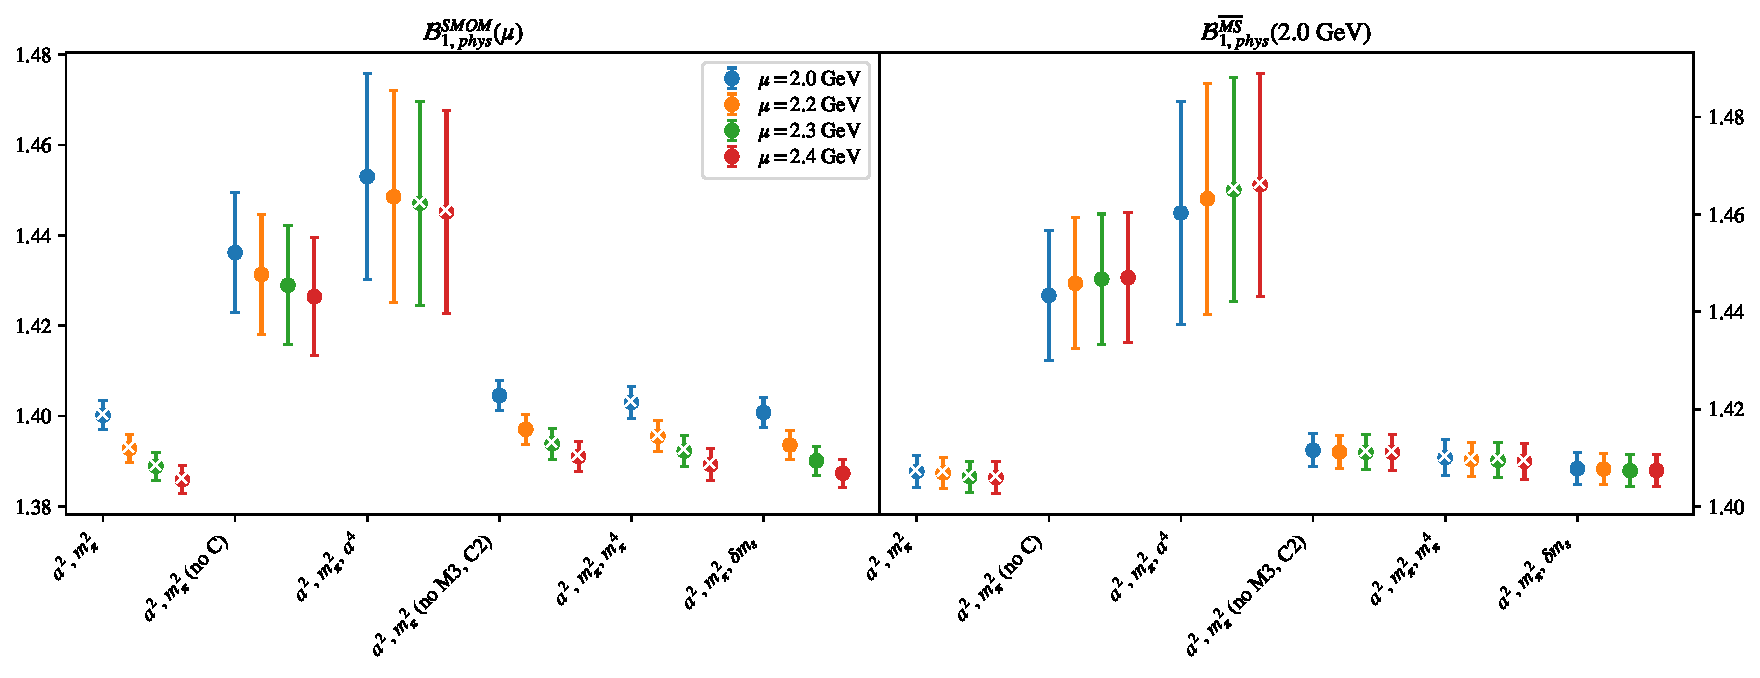
\includegraphics[page=1, width=1.1\textwidth]{VVpAA/NPR/fit_summary_bag.pdf}
\caption{$\mathcal{B}_{1}$\\(left) $\mathcal{B}_{phys}$ in RI/SMOM scheme from fit variations (fits with $p$-value $<0.05$ marked with ``$\times$"). \\(right) $\mathcal{B}_{phys}$ in $\overline{MS}$ computed using $\mathcal{B}^{\overline{MS}} = R^{\overline{MS}\leftarrow SMOM}(2.0)\sigma_{npt}(2.0,\mu) \mathcal{B}^{SMOM}(\mu)$.}
\end{figure}
\clearpage
\begin{figure}
\centering
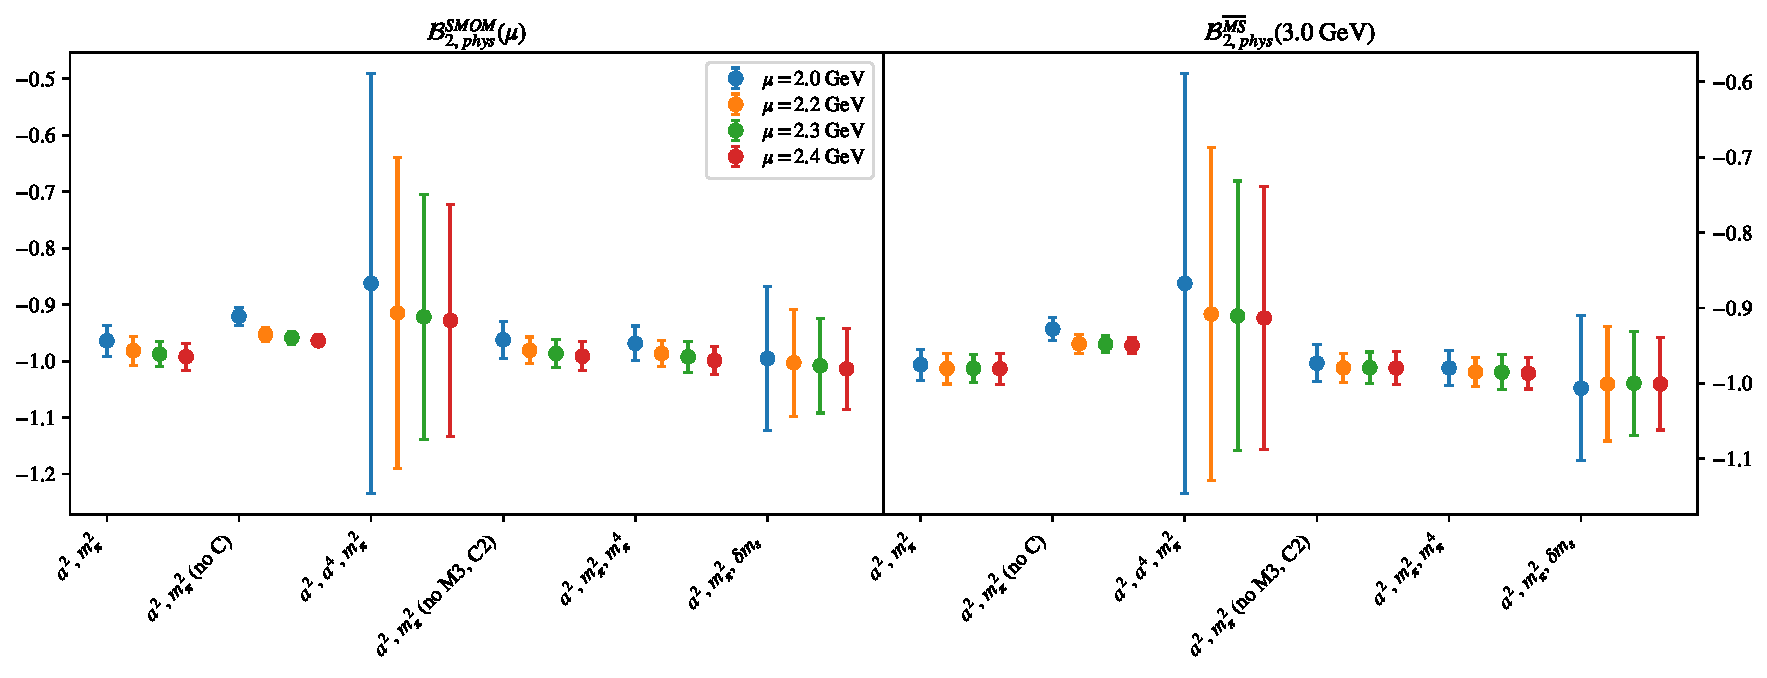
\includegraphics[page=1, width=1.1\textwidth]{VVmAA/NPR/fit_summary_bag.pdf}
\caption{$\mathcal{B}_{2}$\\(left) $\mathcal{B}_{phys}$ in RI/SMOM scheme from fit variations (fits with $p$-value $<0.05$ marked with ``$\times$"). \\(right) $\mathcal{B}_{phys}$ in $\overline{MS}$ computed using $\mathcal{B}^{\overline{MS}} = R^{\overline{MS}\leftarrow SMOM}(3.0)\sigma_{npt}(3.0,\mu) \mathcal{B}^{SMOM}(\mu)$.}
\end{figure}
\clearpage
\begin{figure}
\centering
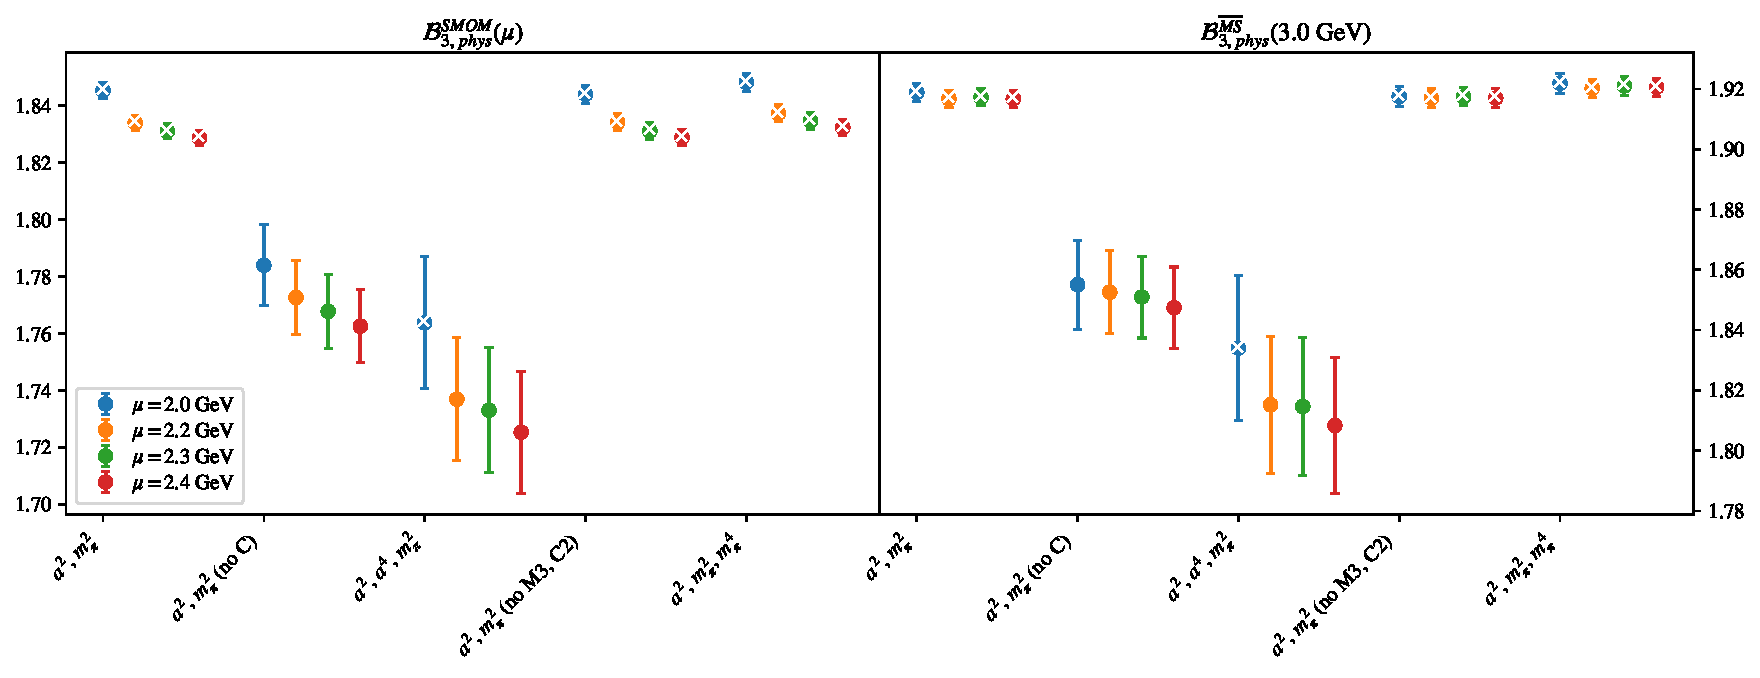
\includegraphics[page=1, width=1.1\textwidth]{SSmPP/NPR/fit_summary_bag.pdf}
\caption{$\mathcal{B}_{3}$\\(left) $\mathcal{B}_{phys}$ in RI/SMOM scheme from fit variations (fits with $p$-value $<0.05$ marked with ``$\times$"). \\(right) $\mathcal{B}_{phys}$ in $\overline{MS}$ computed using $\mathcal{B}^{\overline{MS}} = R^{\overline{MS}\leftarrow SMOM}(3.0)\sigma_{npt}(3.0,\mu) \mathcal{B}^{SMOM}(\mu)$.}
\end{figure}
\clearpage
\begin{figure}
\centering
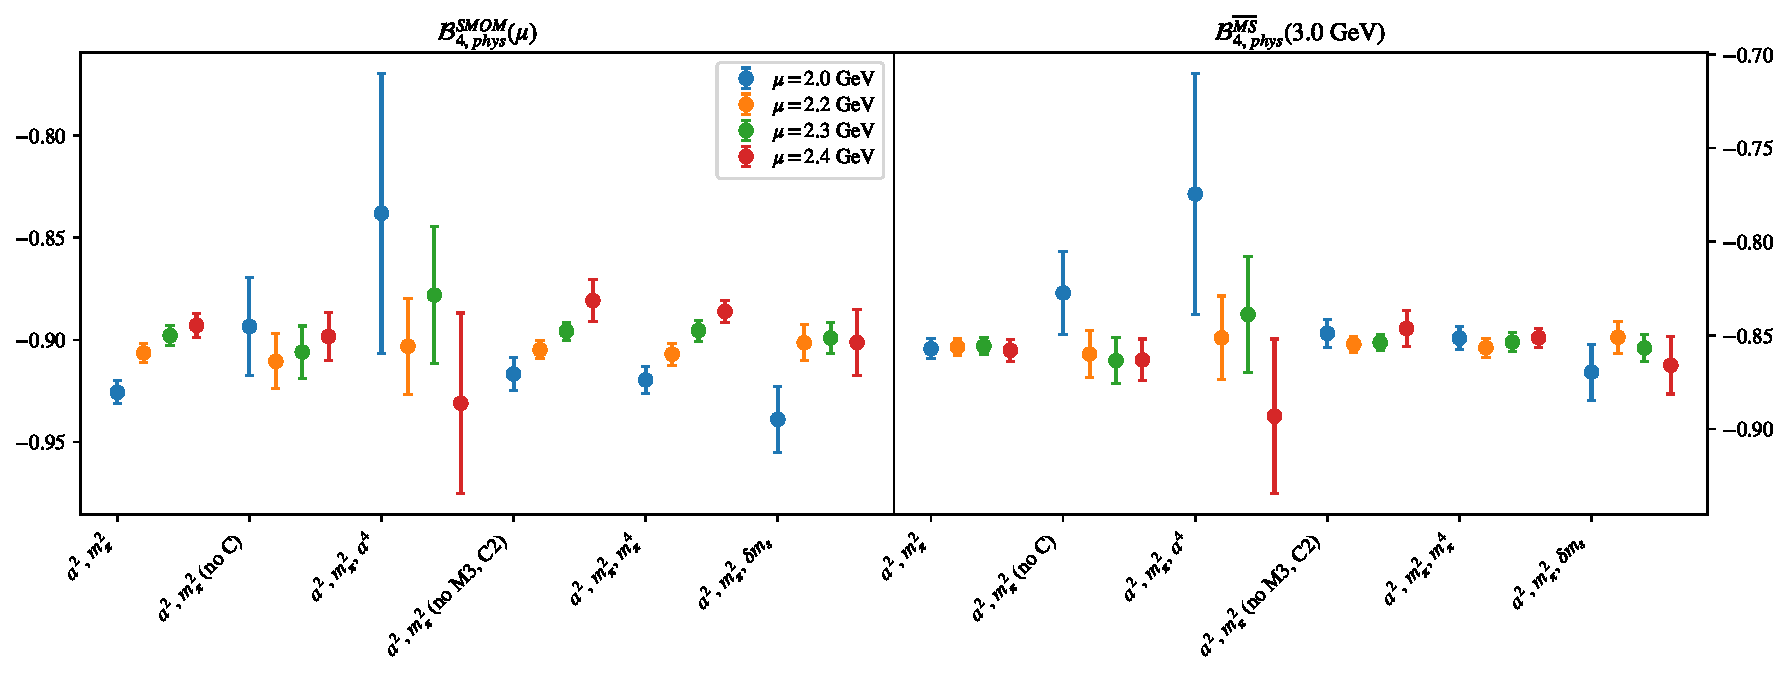
\includegraphics[page=1, width=1.1\textwidth]{SSpPP/NPR/fit_summary_bag.pdf}
\caption{$\mathcal{B}_{4}$\\(left) $\mathcal{B}_{phys}$ in RI/SMOM scheme from fit variations (fits with $p$-value $<0.05$ marked with ``$\times$"). \\(right) $\mathcal{B}_{phys}$ in $\overline{MS}$ computed using $\mathcal{B}^{\overline{MS}} = R^{\overline{MS}\leftarrow SMOM}(3.0)\sigma_{npt}(3.0,\mu) \mathcal{B}^{SMOM}(\mu)$.}
\end{figure}
\clearpage
\begin{figure}
\centering
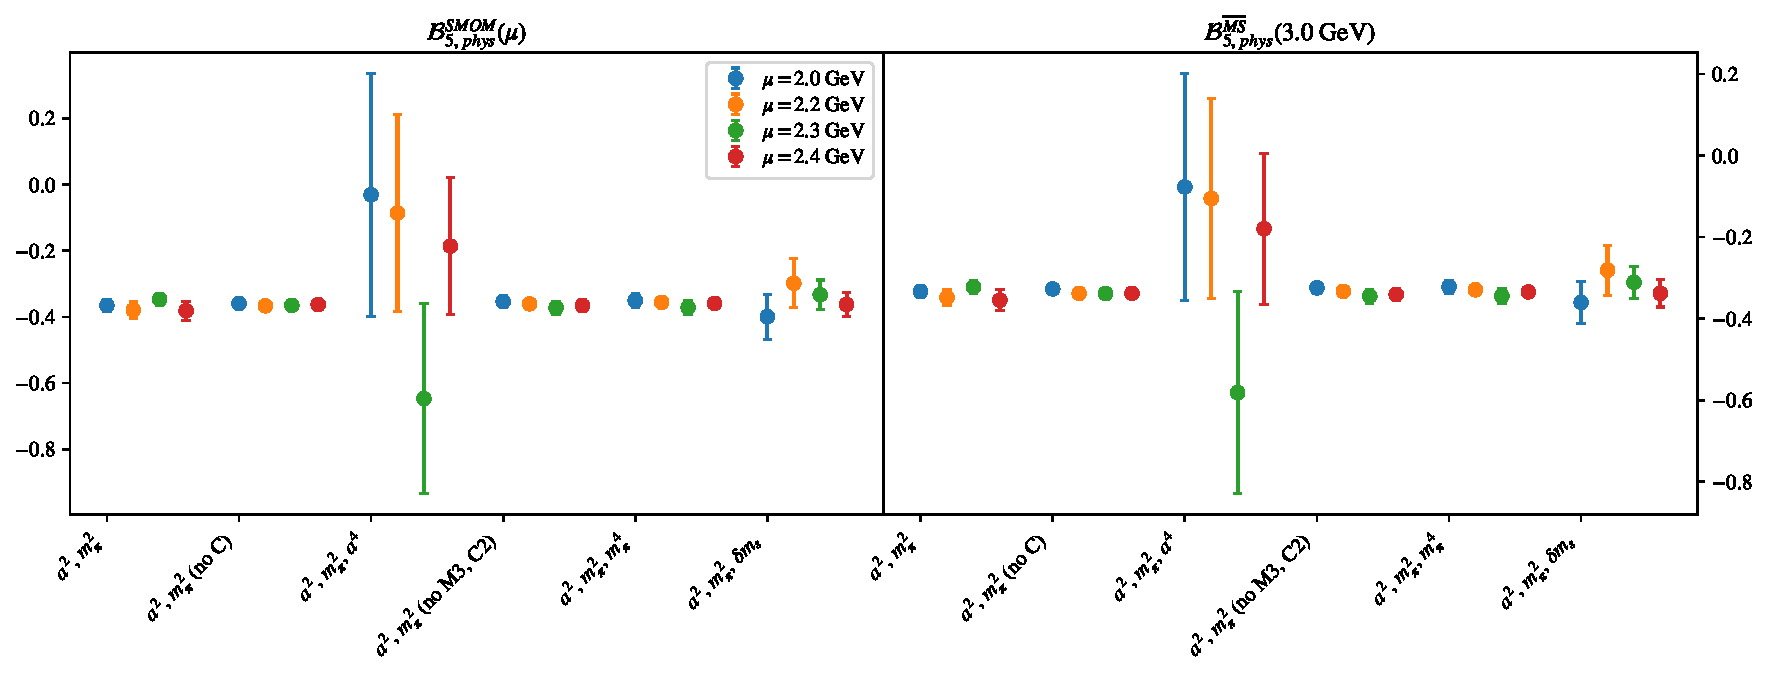
\includegraphics[page=1, width=1.1\textwidth]{TT/NPR/fit_summary_bag.pdf}
\caption{$\mathcal{B}_{5}$\\(left) $\mathcal{B}_{phys}$ in RI/SMOM scheme from fit variations (fits with $p$-value $<0.05$ marked with ``$\times$"). \\(right) $\mathcal{B}_{phys}$ in $\overline{MS}$ computed using $\mathcal{B}^{\overline{MS}} = R^{\overline{MS}\leftarrow SMOM}(3.0)\sigma_{npt}(3.0,\mu) \mathcal{B}^{SMOM}(\mu)$.}
\end{figure}
\clearpage
\section{$\mathcal{B}_1$}
\begin{table}[h!]
\begin{center}
\begin{tabular}{|c|c|c|c|c|c|c|}
\hline
$\mu$ (GeV) & $a^2$, $m_\pi^2$& $a^2$, $m_\pi^2$ (no C)& $a^2$, $m_\pi^2$, $a^4$& $a^2$, $m_\pi^2$ (no M3, C2)& $a^2$, $m_\pi^2$, $m_\pi^4$& $a^2$, $m_\pi^2$, $\delta m_s$\\
\hline
2.0& \hyperlink{VVpAA/NPR/bag_a2m2_20.pdf.1}{\textbf{1.4023(28)}: 2.369 (0.037)} & \hyperlink{VVpAA/NPR/bag_a2m2noC_20.pdf.1}{\textbf{1.417(12)}: 0.897 (0.408)} & \hyperlink{VVpAA/NPR/bag_a2a4m2_20.pdf.1}{\textbf{1.419(21)}: 2.81 (0.024)} & \hyperlink{VVpAA/NPR/bag_a2m2mcut_20.pdf.1}{\textbf{1.4081(32)}: 0.284 (0.837)} & \hyperlink{VVpAA/NPR/bag_a2m2m4_20.pdf.1}{\textbf{1.4081(33)}: 1.051 (0.379)} & \hyperlink{VVpAA/NPR/bag_a2m2delm_20.pdf.1}{\textbf{1.3999(33)}: 2.41 (0.047)}\\
2.2& \hyperlink{VVpAA/NPR/bag_a2m2_22.pdf.1}{\textbf{1.3949(28)}: 2.686 (0.02)} & \hyperlink{VVpAA/NPR/bag_a2m2noC_22.pdf.1}{\textbf{1.412(12)}: 1.029 (0.357)} & \hyperlink{VVpAA/NPR/bag_a2a4m2_22.pdf.1}{\textbf{1.415(21)}: 3.131 (0.014)} & \hyperlink{VVpAA/NPR/bag_a2m2mcut_22.pdf.1}{\textbf{1.4010(32)}: 0.415 (0.742)} & \hyperlink{VVpAA/NPR/bag_a2m2m4_22.pdf.1}{\textbf{1.4009(33)}: 1.272 (0.278)} & \hyperlink{VVpAA/NPR/bag_a2m2delm_22.pdf.1}{\textbf{1.3922(33)}: 2.622 (0.033)}\\
2.3& \hyperlink{VVpAA/NPR/bag_a2m2_23.pdf.1}{\textbf{1.3913(27)}: 2.92 (0.012)} & \hyperlink{VVpAA/NPR/bag_a2m2noC_23.pdf.1}{\textbf{1.409(12)}: 1.106 (0.331)} & \hyperlink{VVpAA/NPR/bag_a2a4m2_23.pdf.1}{\textbf{1.413(21)}: 3.381 (0.009)} & \hyperlink{VVpAA/NPR/bag_a2m2mcut_23.pdf.1}{\textbf{1.3977(32)}: 0.499 (0.683)} & \hyperlink{VVpAA/NPR/bag_a2m2m4_23.pdf.1}{\textbf{1.3975(33)}: 1.443 (0.217)} & \hyperlink{VVpAA/NPR/bag_a2m2delm_23.pdf.1}{\textbf{1.3885(32)}: 2.792 (0.025)}\\
2.4& \hyperlink{VVpAA/NPR/bag_a2m2_24.pdf.1}{\textbf{1.3884(27)}: 3.03 (0.01)} & \hyperlink{VVpAA/NPR/bag_a2m2noC_24.pdf.1}{\textbf{1.407(12)}: 1.156 (0.315)} & \hyperlink{VVpAA/NPR/bag_a2a4m2_24.pdf.1}{\textbf{1.411(20)}: 3.505 (0.007)} & \hyperlink{VVpAA/NPR/bag_a2m2mcut_24.pdf.1}{\textbf{1.3949(32)}: 0.528 (0.663)} & \hyperlink{VVpAA/NPR/bag_a2m2m4_24.pdf.1}{\textbf{1.3946(33)}: 1.509 (0.196)} & \hyperlink{VVpAA/NPR/bag_a2m2delm_24.pdf.1}{\textbf{1.3854(32)}: 2.879 (0.021)}\\
\hline
\end{tabular}
\caption{Physical point value from chiral and continuum extrapolation at renormalisation scale $\mu$. Entries are \textbf{value(error)}: $\chi^2/\text{DOF}$ ($p$-value).}
\end{center}
\end{table}
\begin{table}[h!]
\begin{center}
\begin{tabular}{|c c|c|c|c|c|c|c|}
\hline
$\mu$ (GeV) &  & $a^2$, $m_\pi^2$& $a^2$, $m_\pi^2$ (no C)& $a^2$, $m_\pi^2$, $a^4$& $a^2$, $m_\pi^2$ (no M3, C2)& $a^2$, $m_\pi^2$, $m_\pi^4$& $a^2$, $m_\pi^2$, $\delta m_s$\\
\hline
\multirow{3}{0.5in}{2.0} & $\alpha$ & 0.138(10)& 0.065(76)& -0.01(19)& 0.119(11)& 0.120(11)& 0.146(11)\\
 & $\beta$ & 0.00400(21)& 0.00326(42)& 0.00408(23)& 0.00286(42)& 0.0005(12)& 0.00415(23)\\
 & $\gamma$ &  &  & 0.31(40)&  & 0.00031(11)& -0.0048(33)\\
\hline
\multirow{3}{0.5in}{2.2} & $\alpha$ & 0.143(10)& 0.056(75)& -0.04(19)& 0.123(11)& 0.124(11)& 0.152(11)\\
 & $\beta$ & 0.00391(20)& 0.00314(41)& 0.00401(23)& 0.00272(41)& 0.0003(12)& 0.00408(23)\\
 & $\gamma$ &  &  & 0.38(40)&  & 0.00032(11)& -0.0055(33)\\
\hline
\multirow{3}{0.5in}{2.3} & $\alpha$ & 0.146(10)& 0.052(74)& -0.06(19)& 0.125(11)& 0.126(11)& 0.155(11)\\
 & $\beta$ & 0.00388(20)& 0.00308(41)& 0.00399(23)& 0.00266(41)& 0.0001(12)& 0.00407(22)\\
 & $\gamma$ &  &  & 0.41(39)&  & 0.00033(10)& -0.0059(33)\\
\hline
\multirow{3}{0.5in}{2.4} & $\alpha$ & 0.1468(99)& 0.050(74)& -0.06(19)& 0.125(11)& 0.127(11)& 0.156(11)\\
 & $\beta$ & 0.00386(20)& 0.00305(40)& 0.00397(22)& 0.00263(41)& 0.00009(126)& 0.00405(22)\\
 & $\gamma$ &  &  & 0.42(39)&  & 0.00033(10)& -0.0061(32)\\
\hline
\end{tabular}
\caption{Fit values of coefficients in $Q = Q_{phys} + \mathbf{\alpha} a^2 + \mathbf{\beta}\left(\frac{m_\pi^2}{f_\pi^2}-\frac{m_{\pi,PDG}^2}{f_\pi^2}\right) + \gamma(\ldots)$}
\end{center}
\end{table}
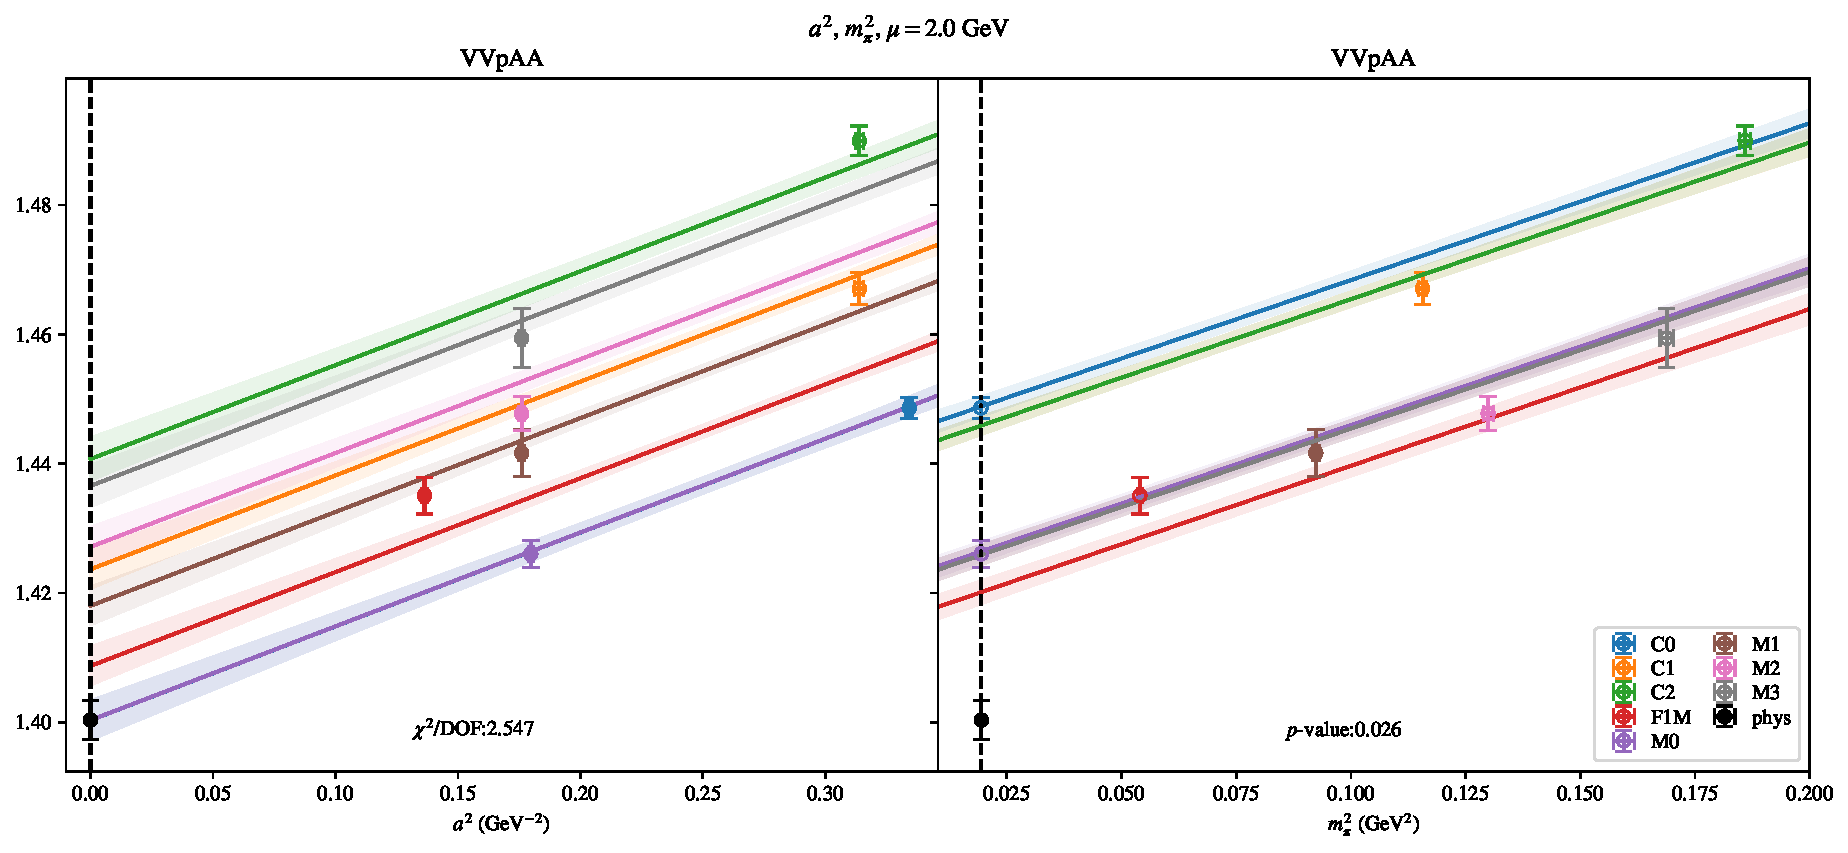
\includepdf[link, pages=-]{VVpAA/NPR/bag_a2m2_20.pdf}
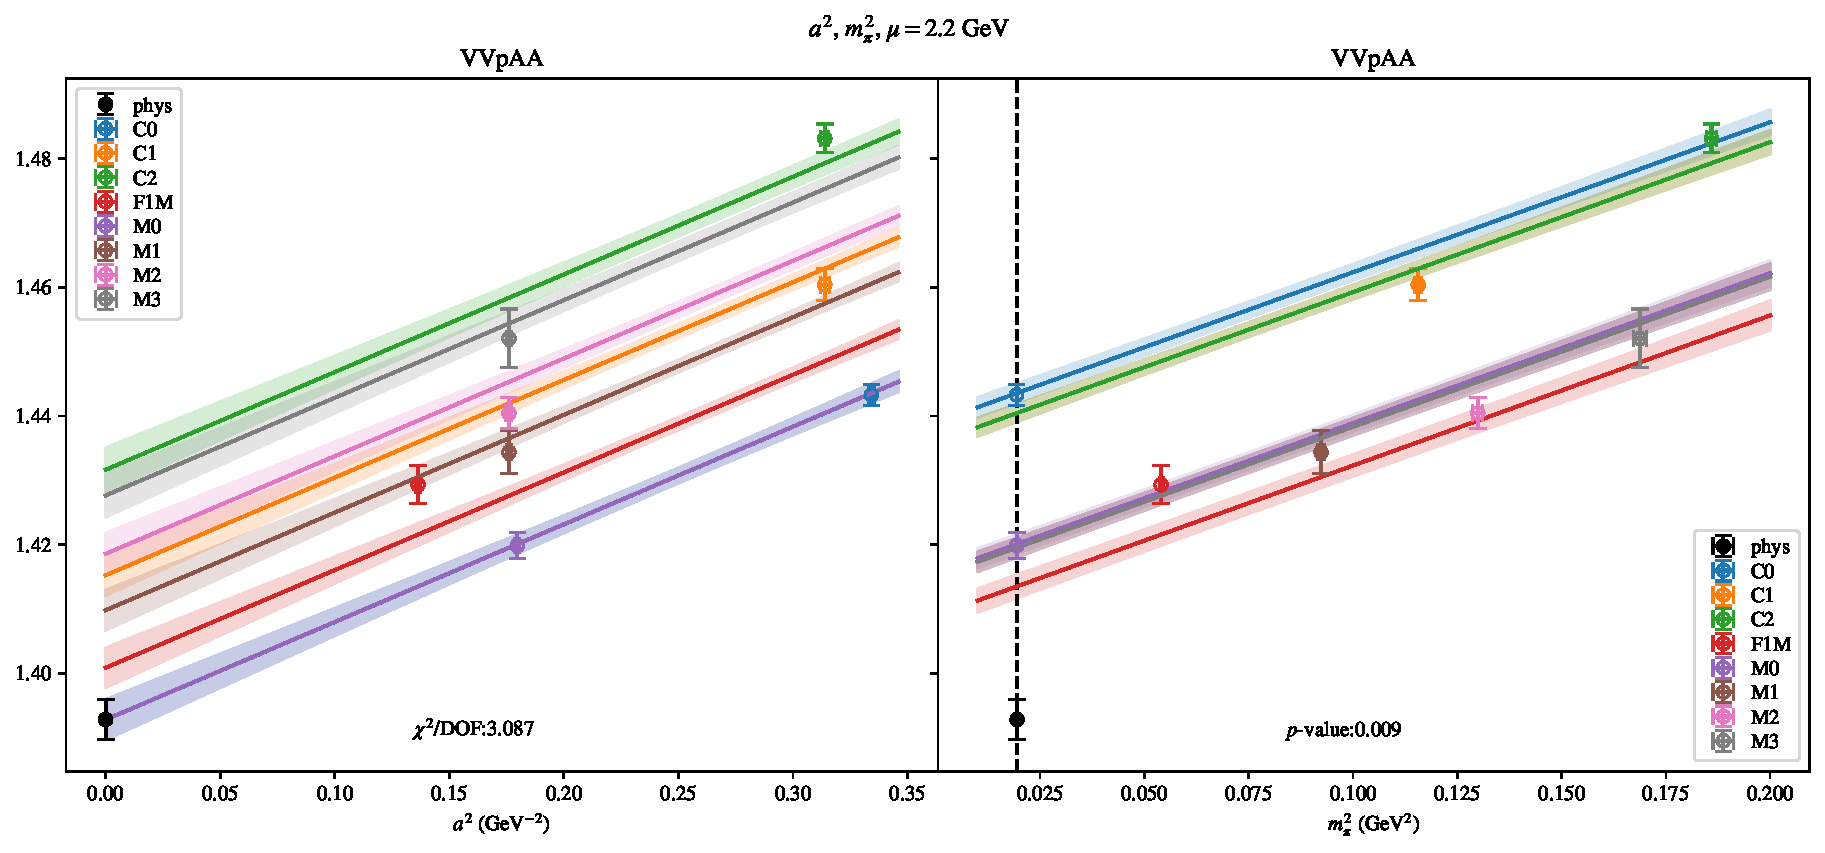
\includepdf[link, pages=-]{VVpAA/NPR/bag_a2m2_22.pdf}
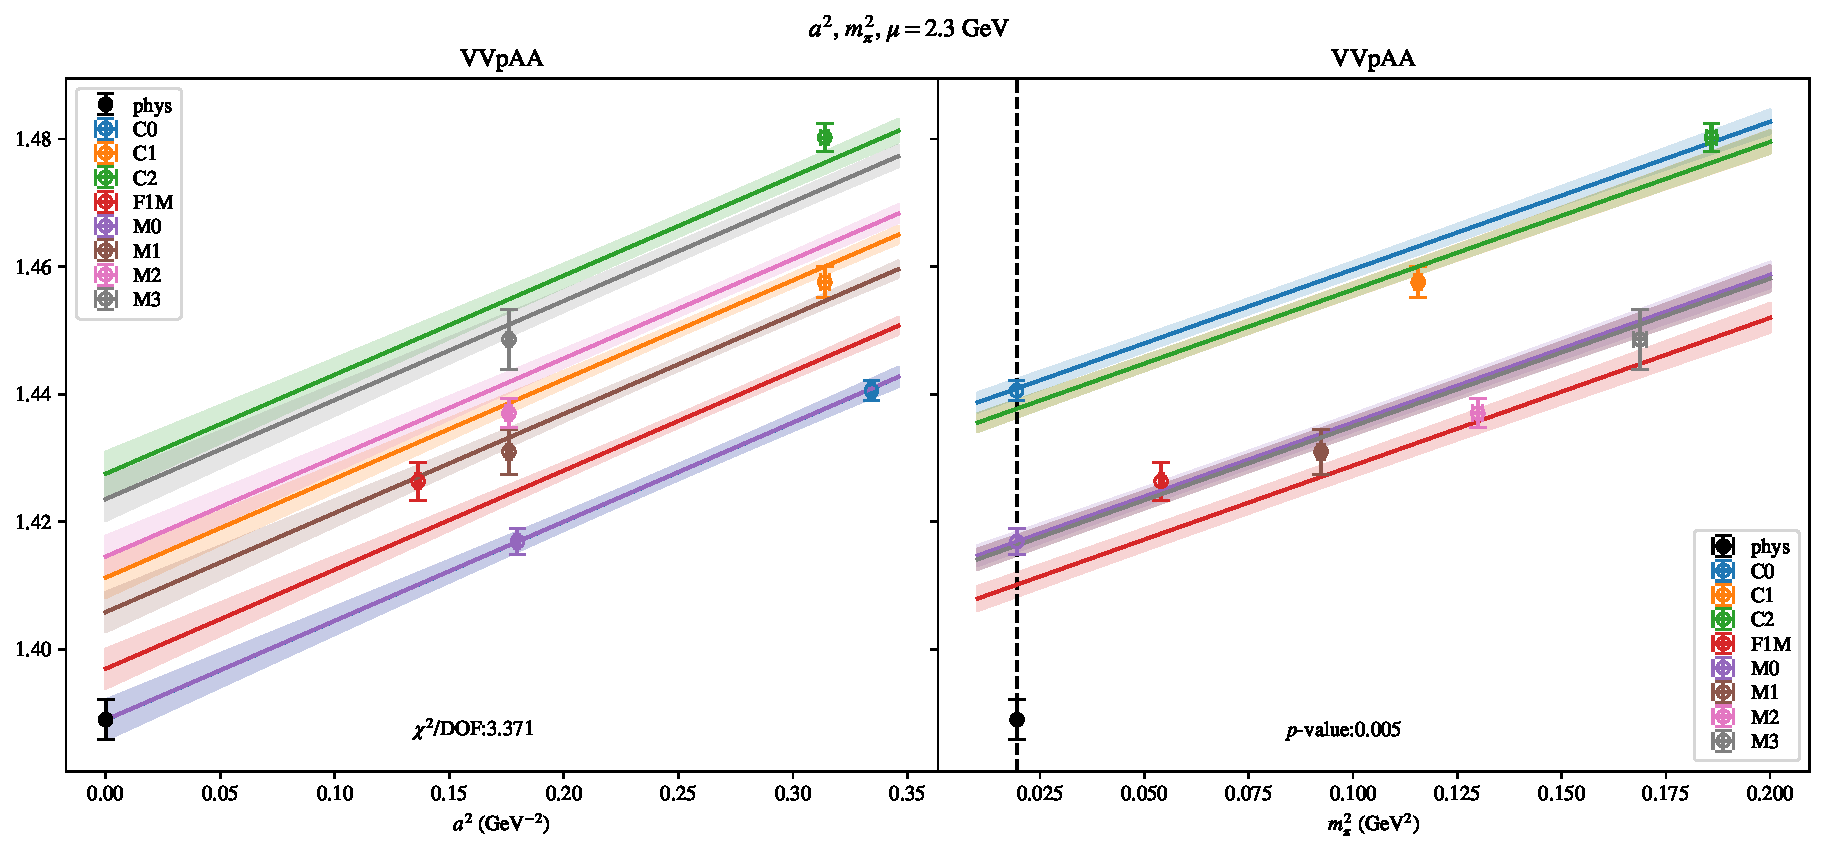
\includepdf[link, pages=-]{VVpAA/NPR/bag_a2m2_23.pdf}
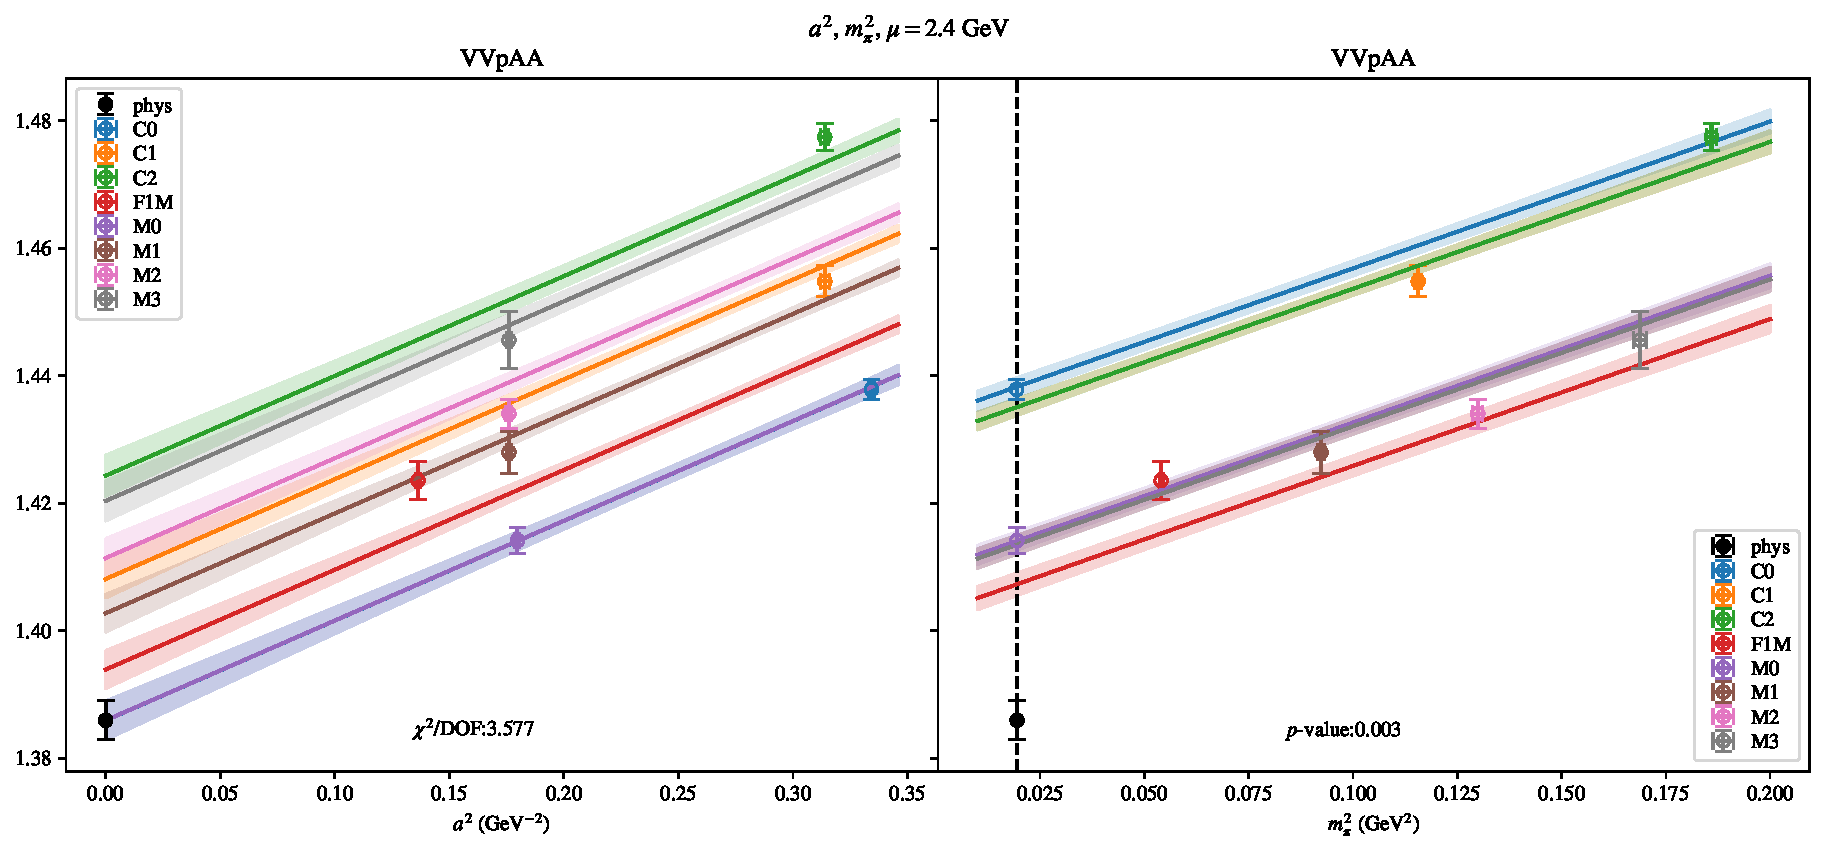
\includepdf[link, pages=-]{VVpAA/NPR/bag_a2m2_24.pdf}
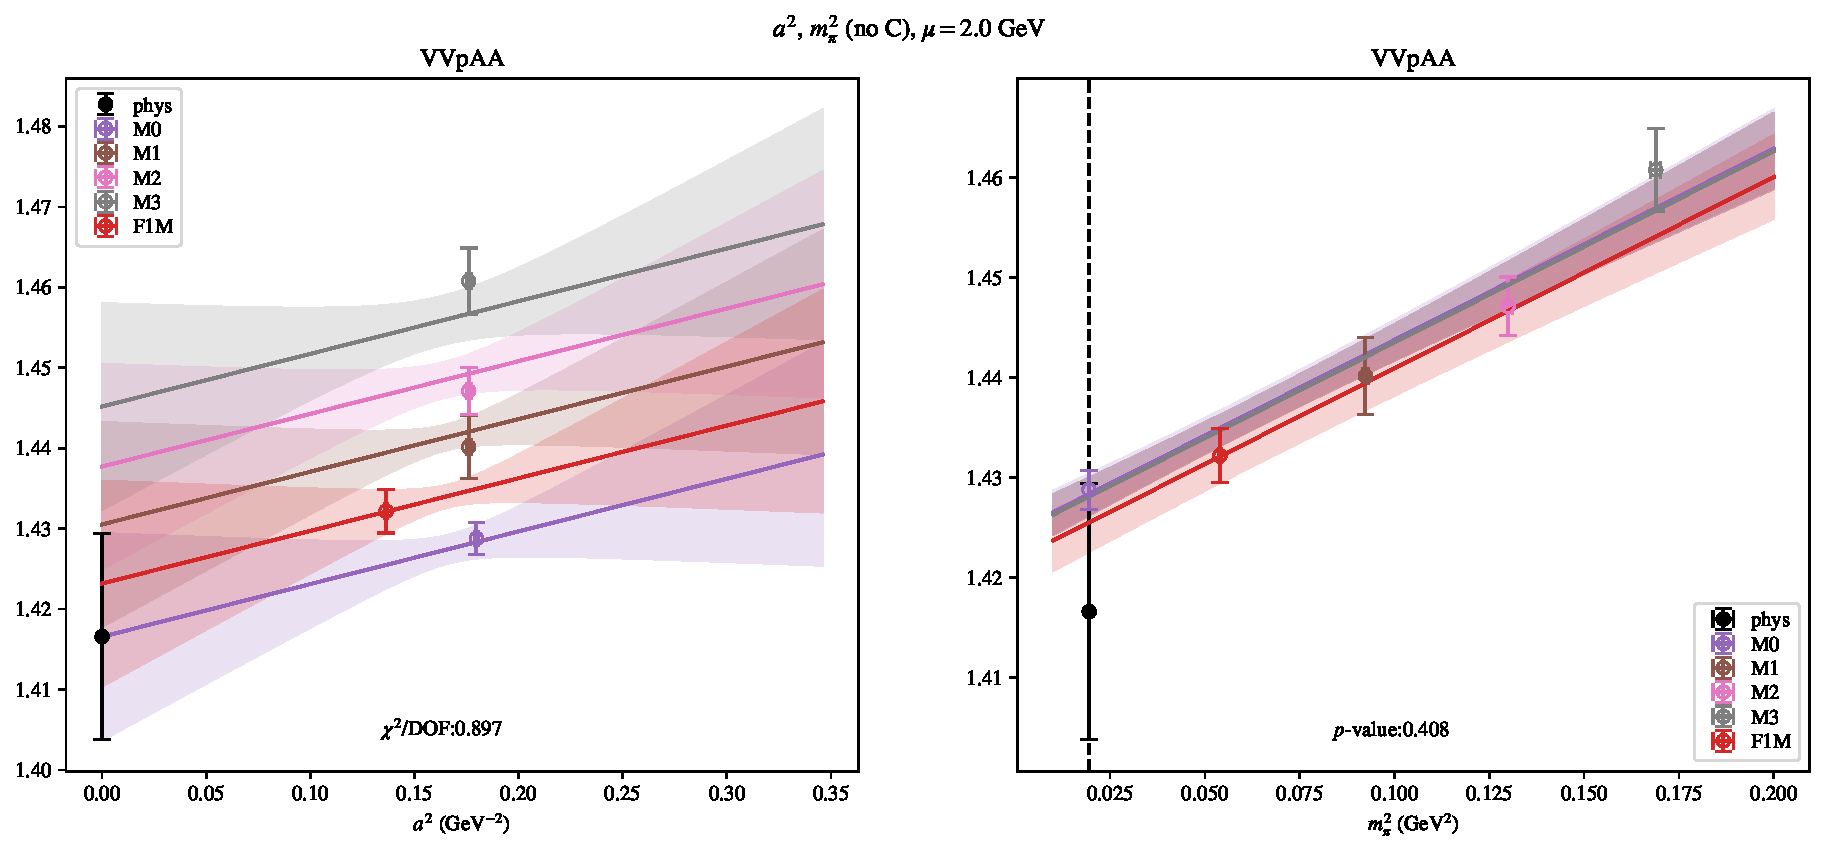
\includepdf[link, pages=-]{VVpAA/NPR/bag_a2m2noC_20.pdf}
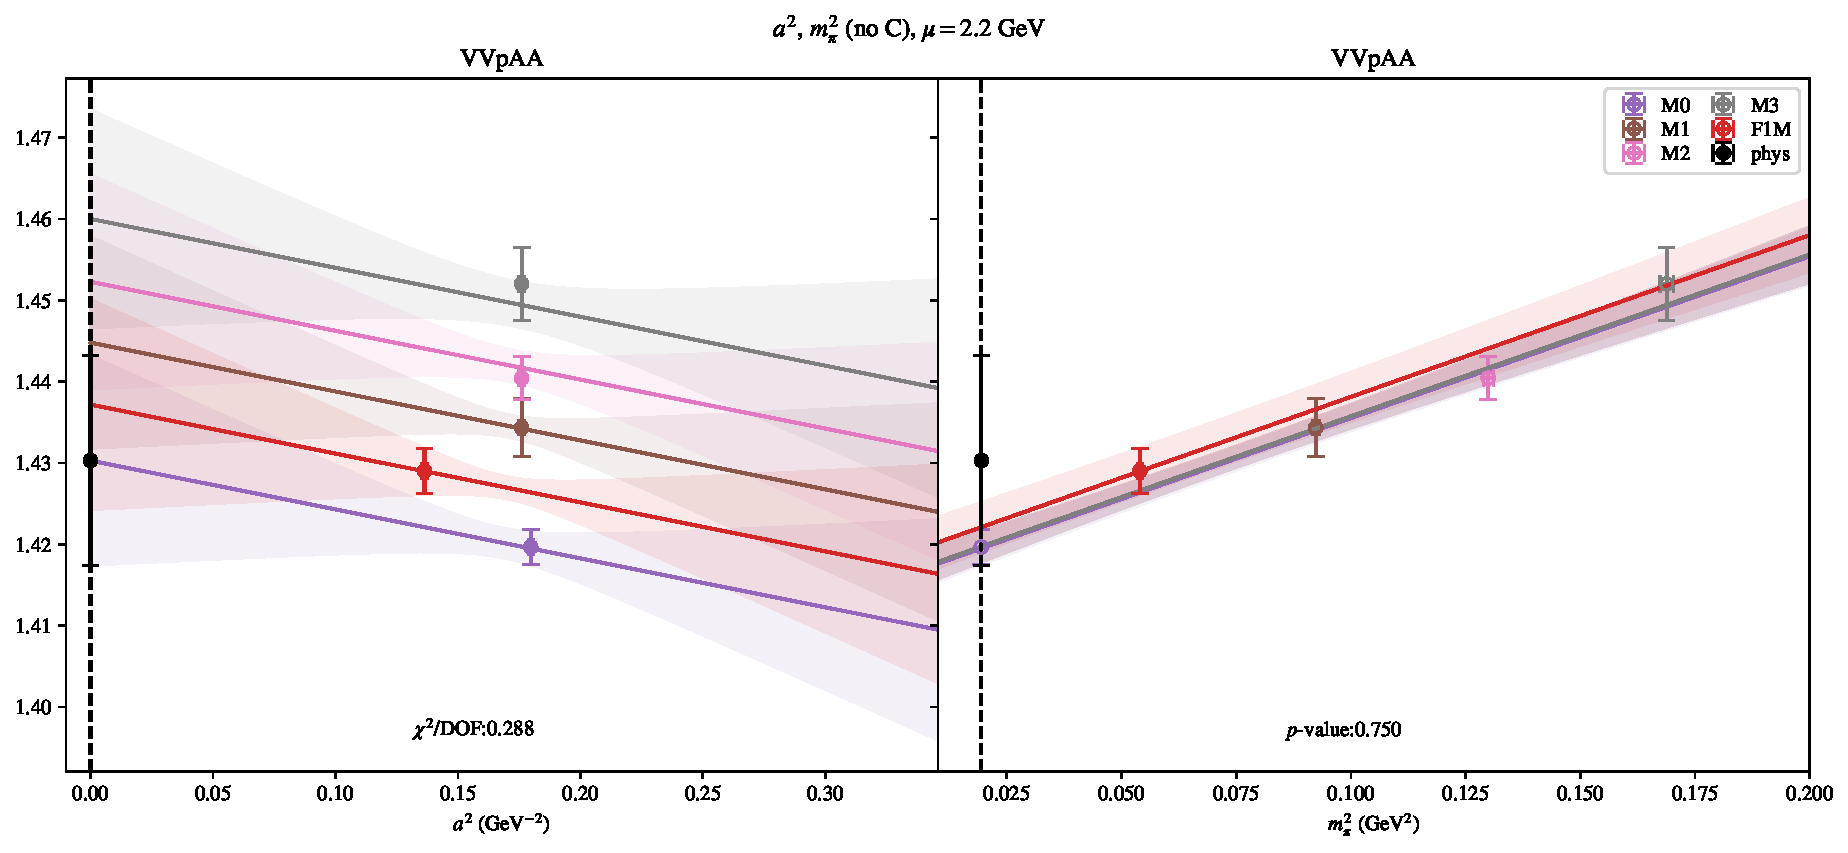
\includepdf[link, pages=-]{VVpAA/NPR/bag_a2m2noC_22.pdf}
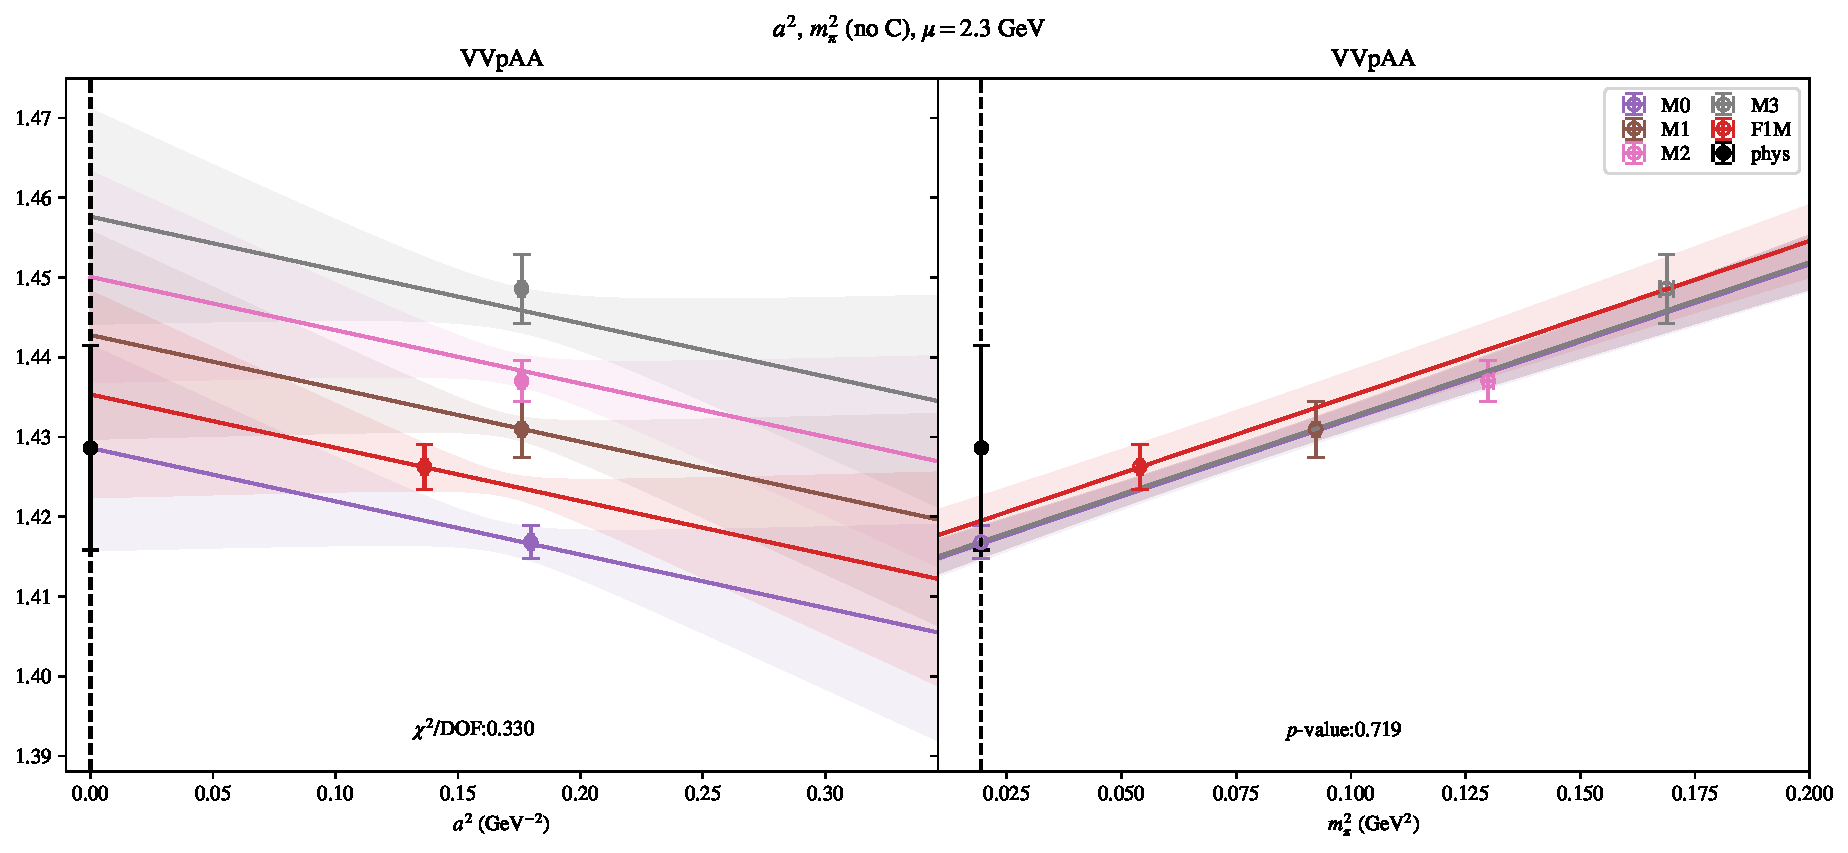
\includepdf[link, pages=-]{VVpAA/NPR/bag_a2m2noC_23.pdf}
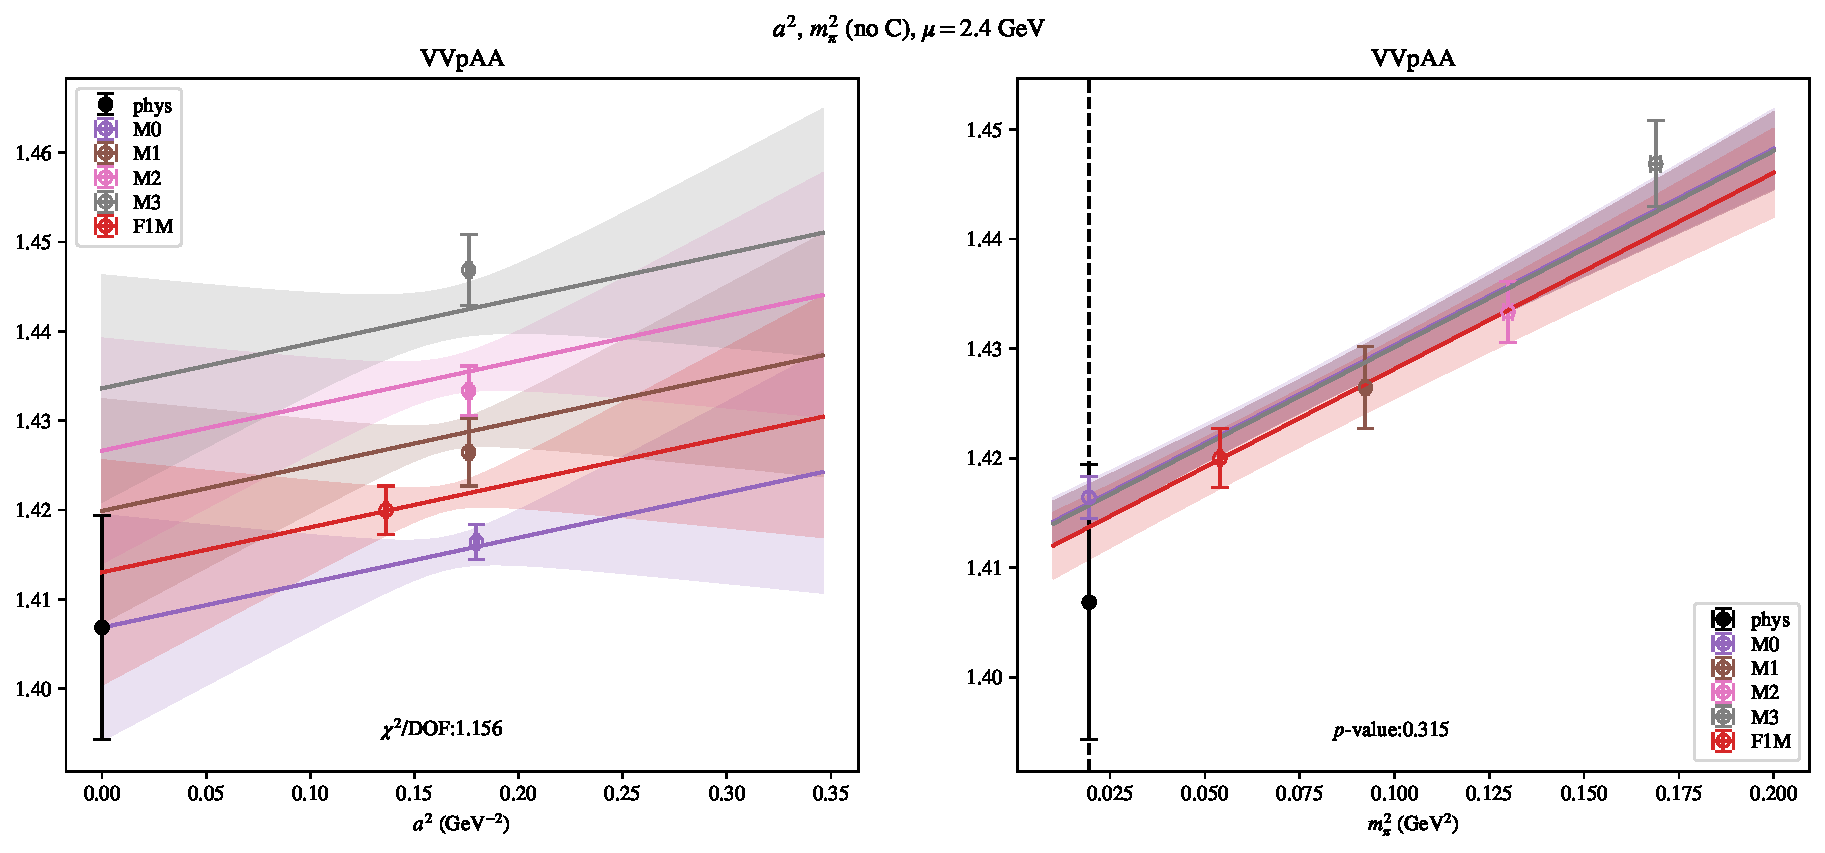
\includepdf[link, pages=-]{VVpAA/NPR/bag_a2m2noC_24.pdf}
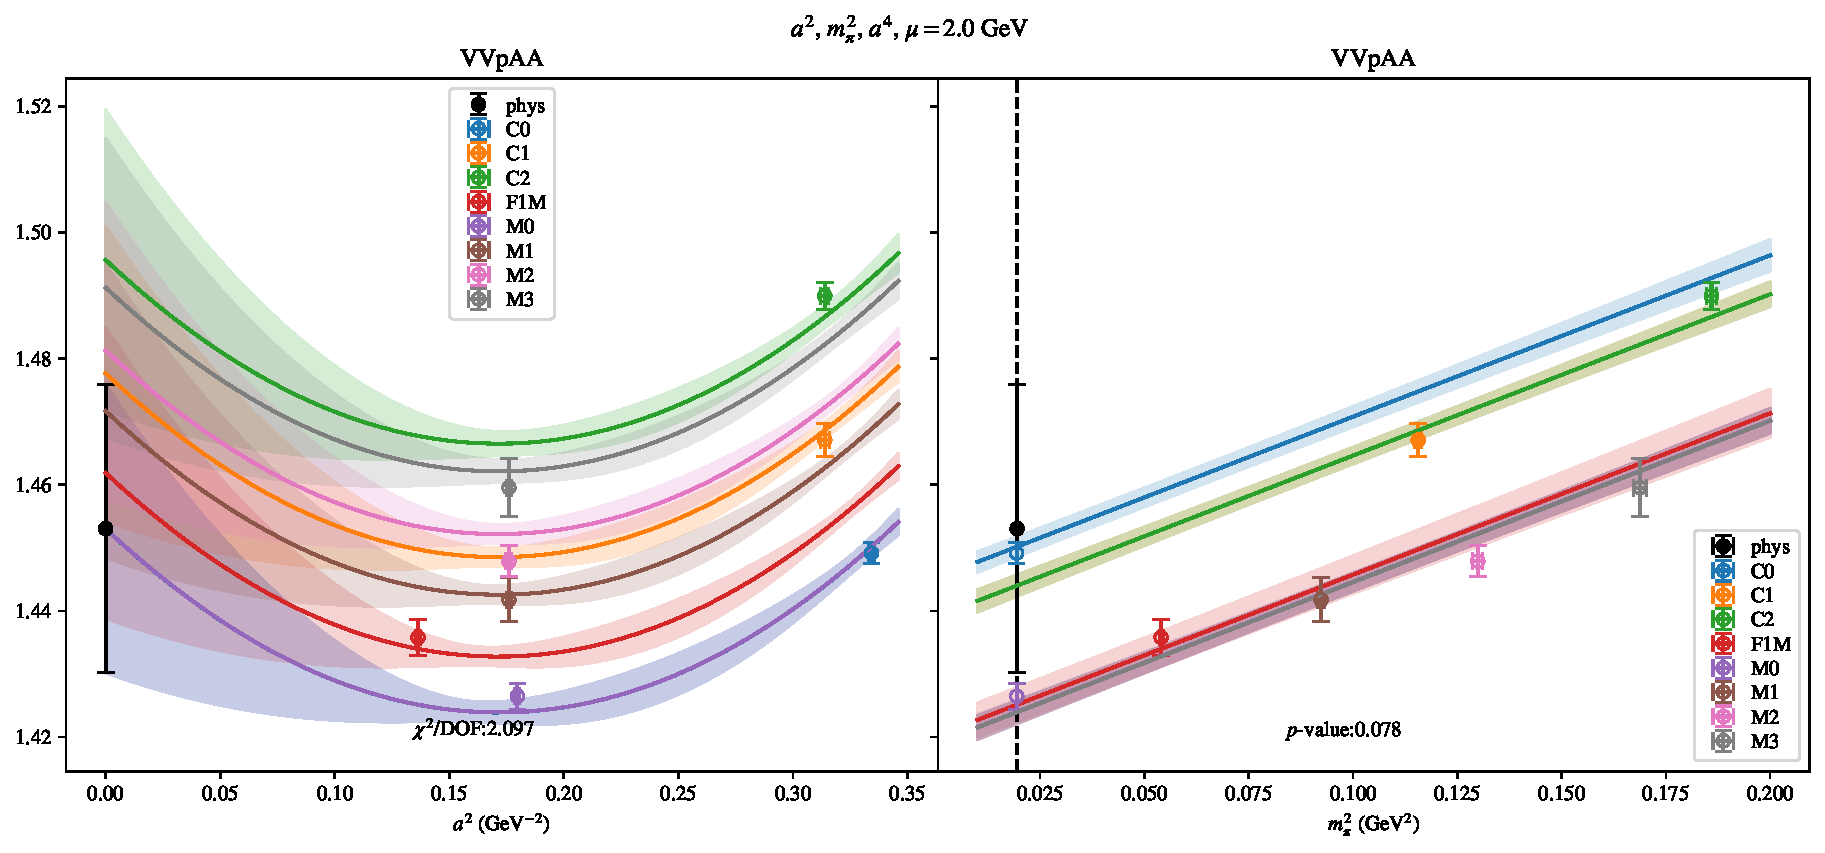
\includepdf[link, pages=-]{VVpAA/NPR/bag_a2a4m2_20.pdf}
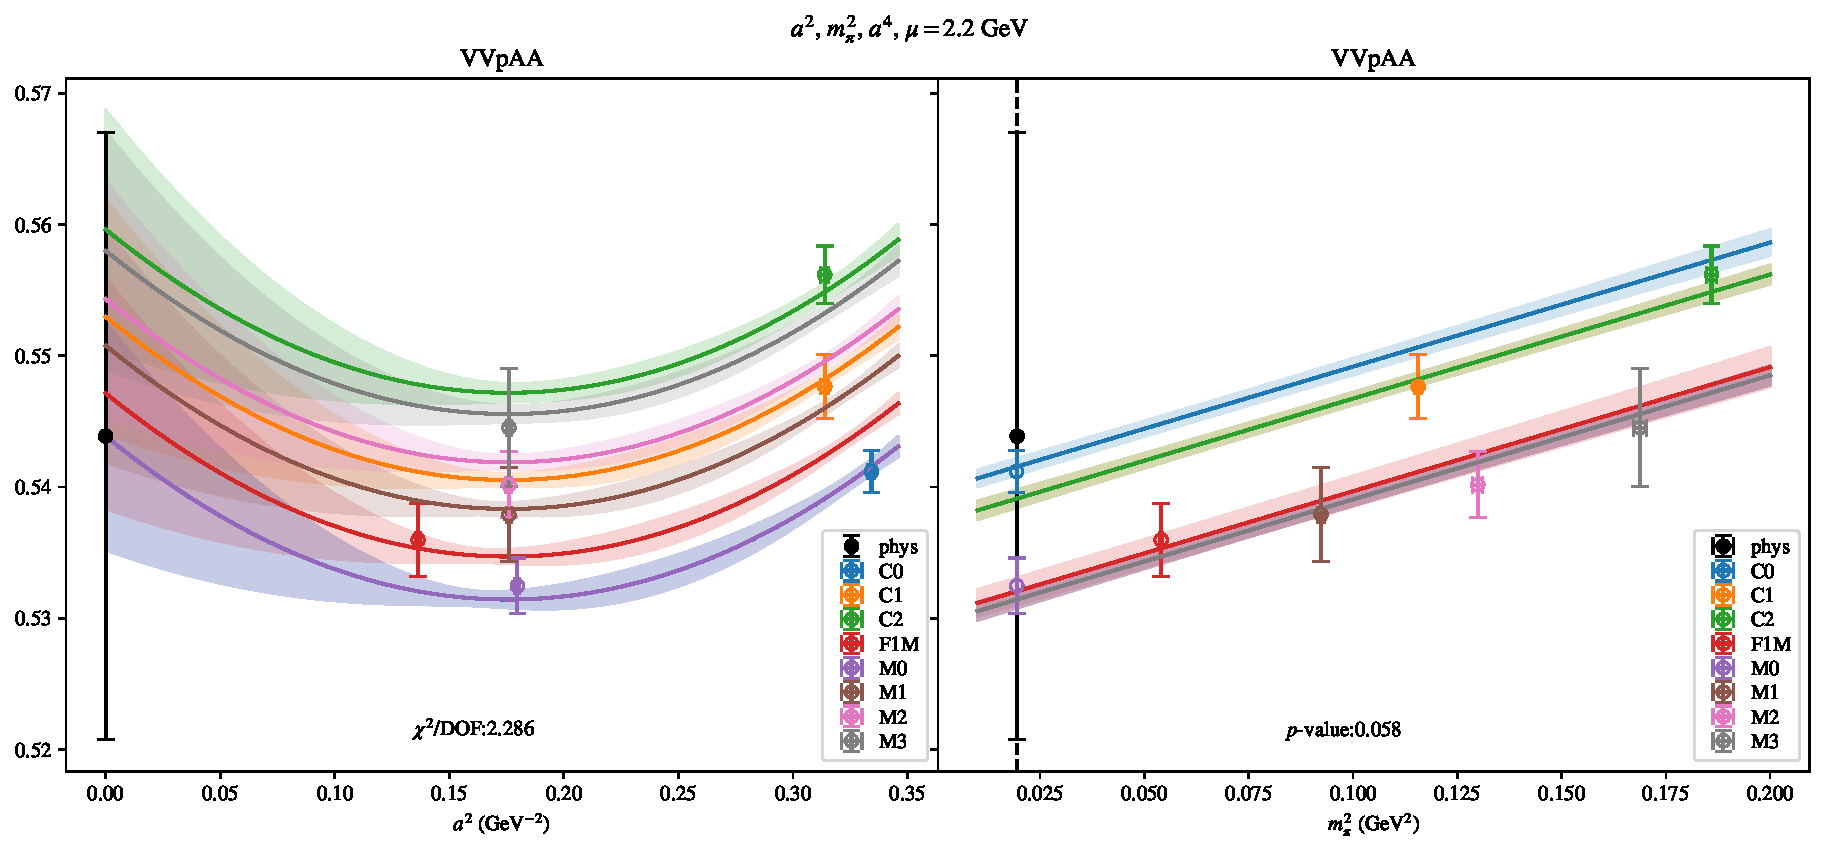
\includepdf[link, pages=-]{VVpAA/NPR/bag_a2a4m2_22.pdf}
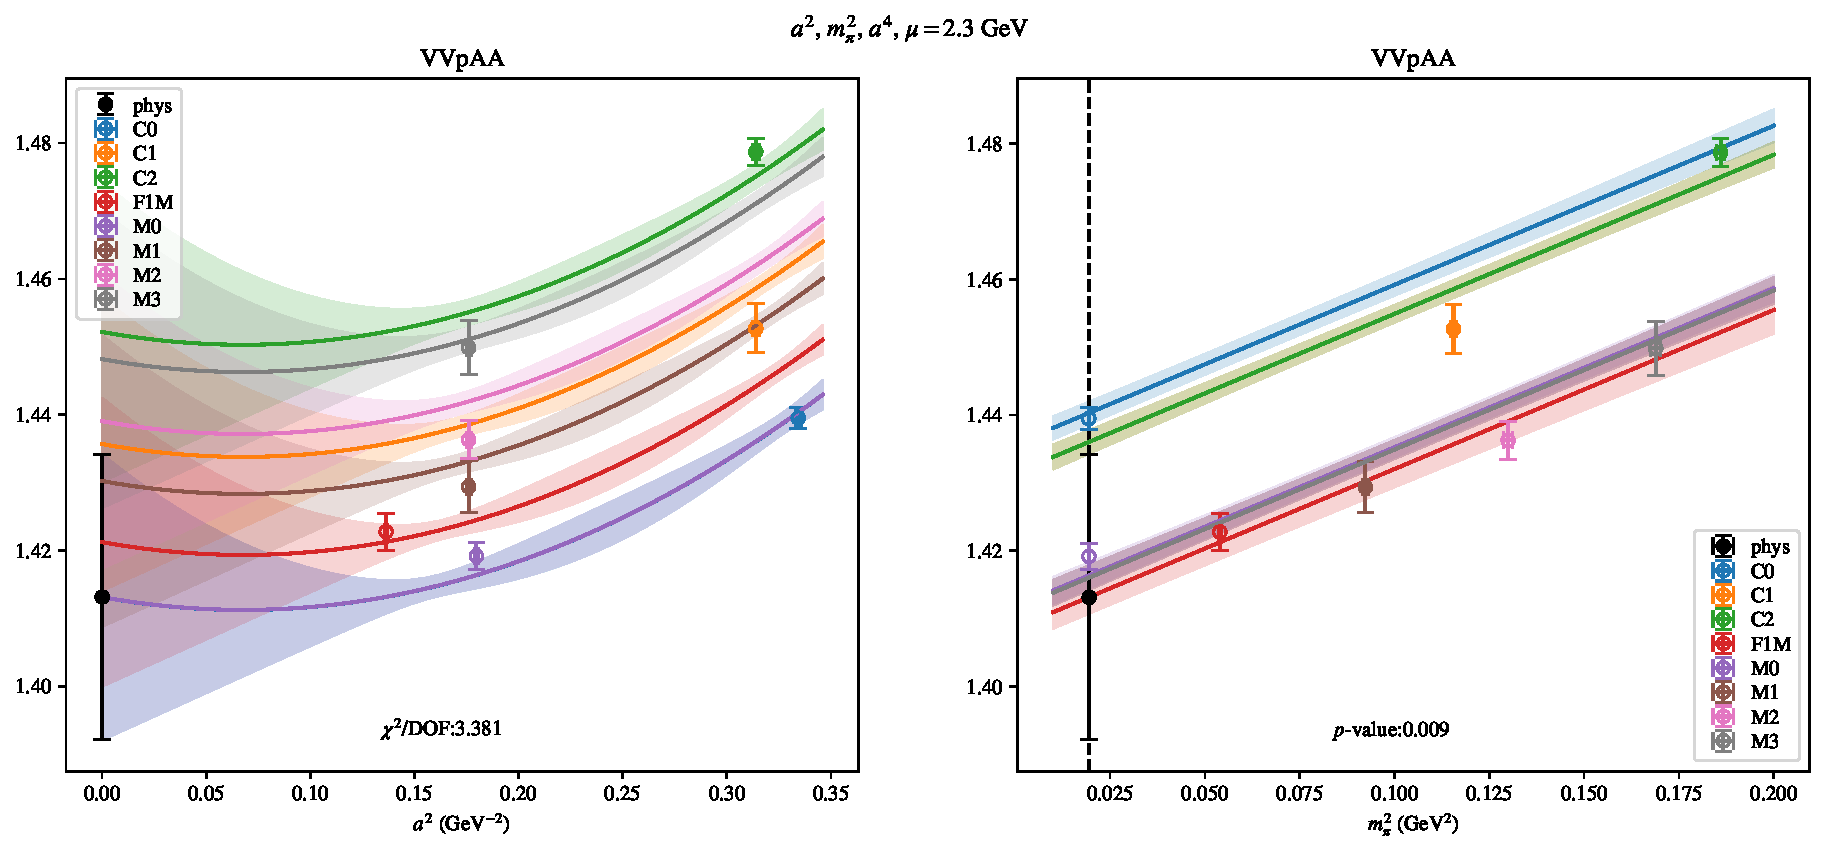
\includepdf[link, pages=-]{VVpAA/NPR/bag_a2a4m2_23.pdf}
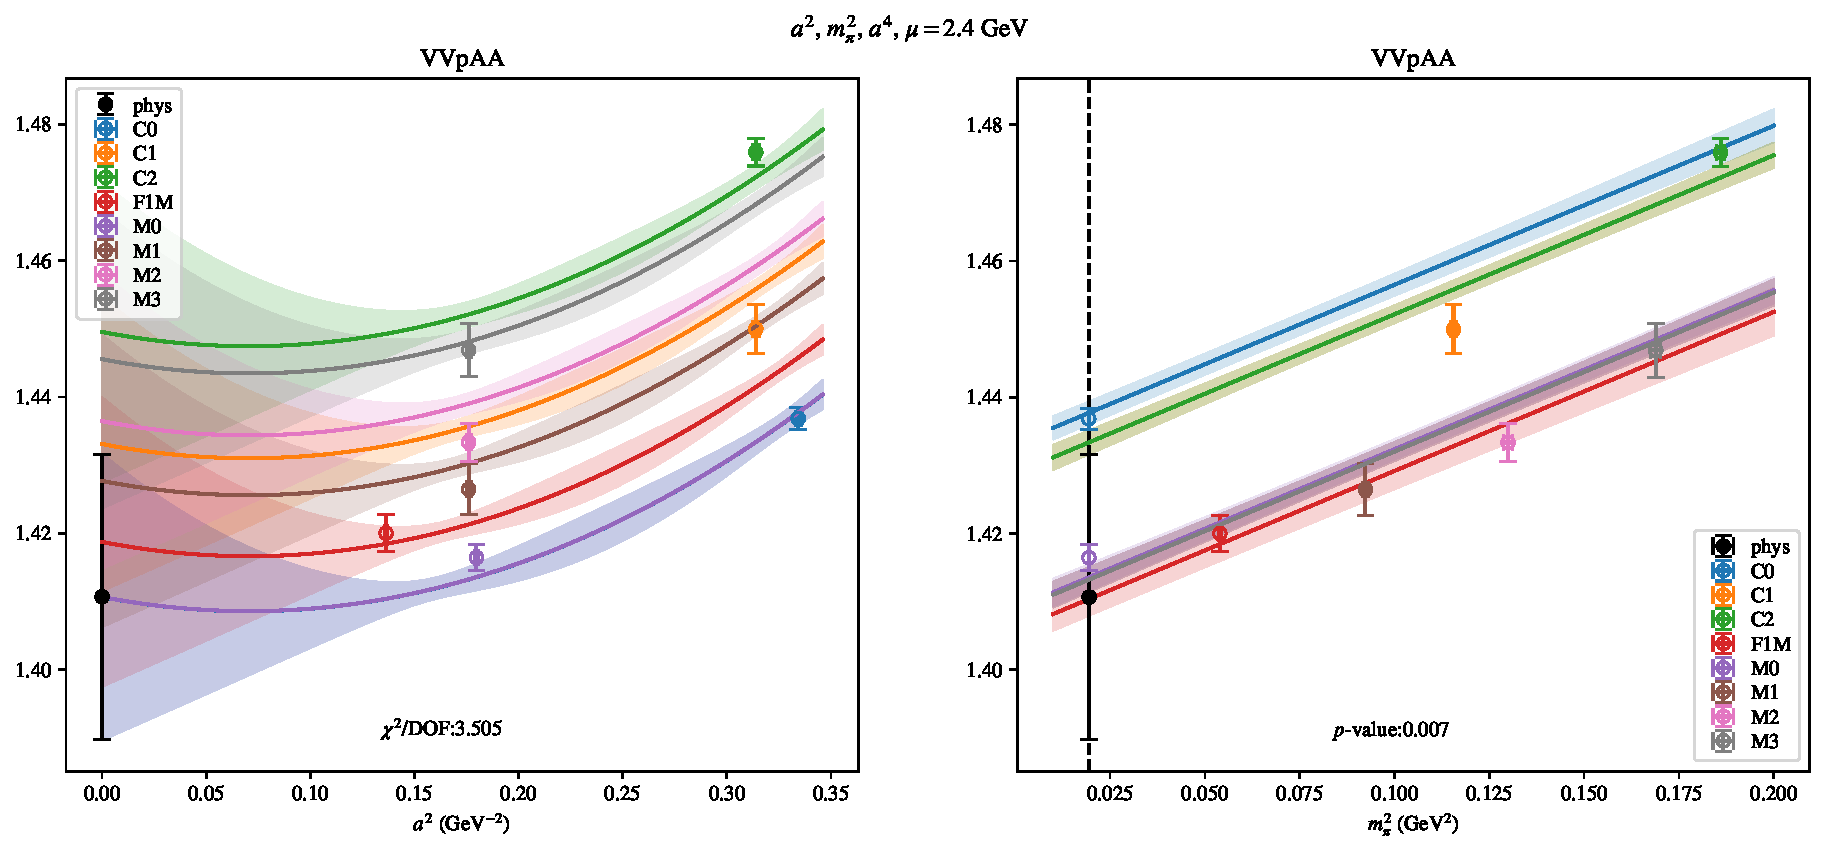
\includepdf[link, pages=-]{VVpAA/NPR/bag_a2a4m2_24.pdf}
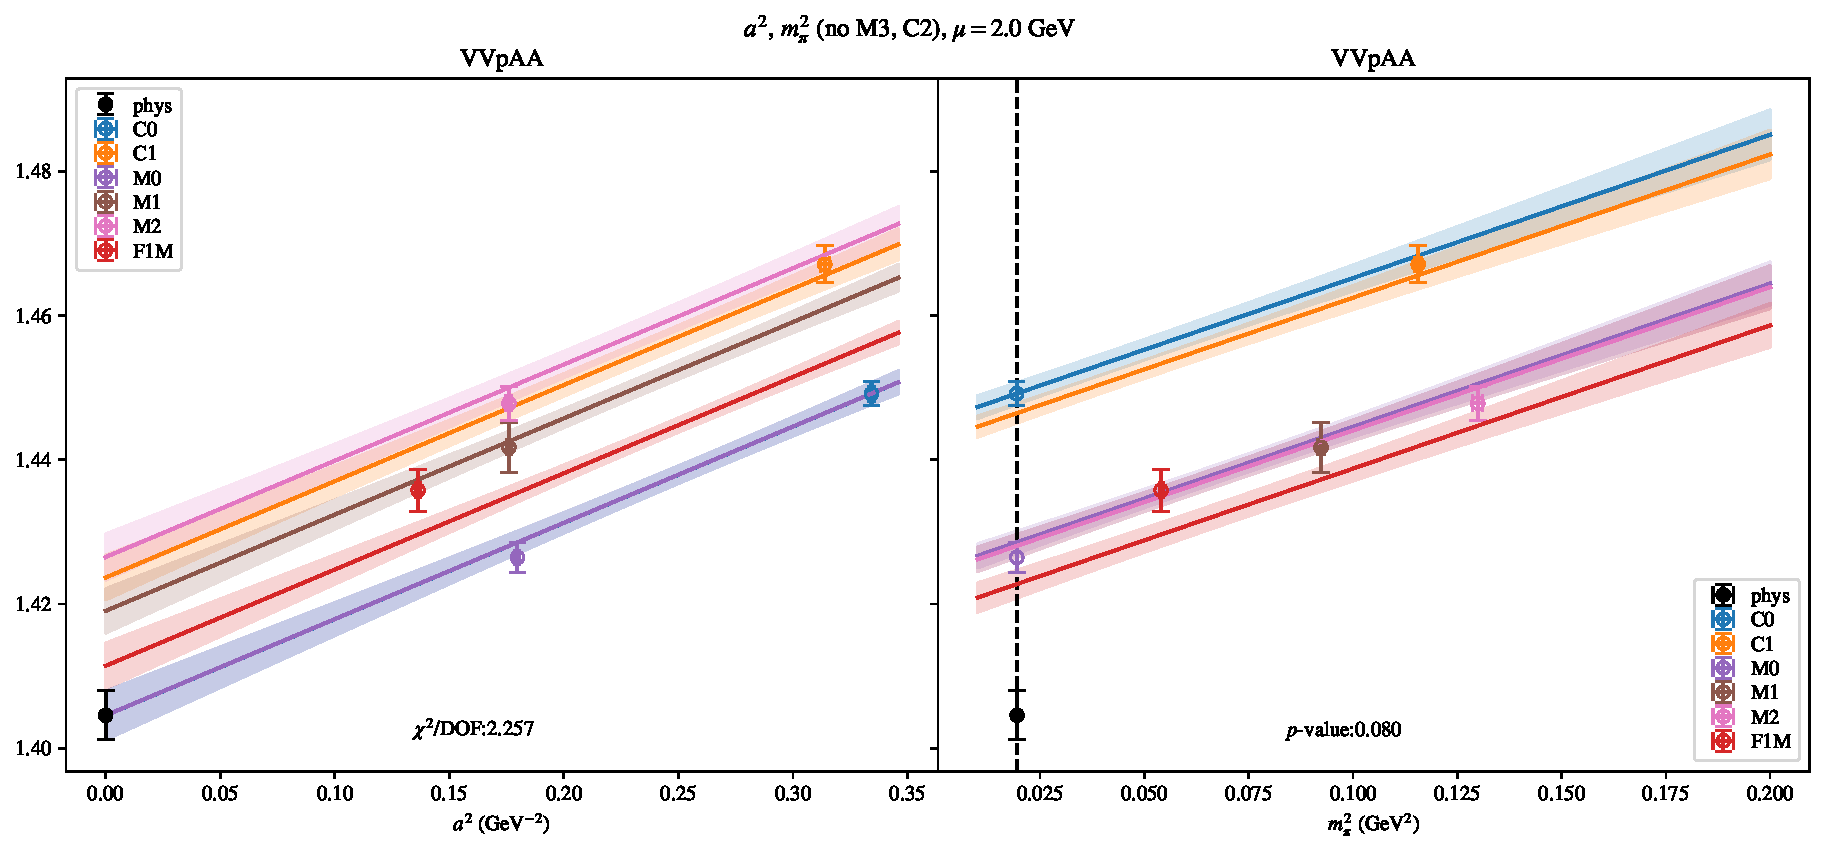
\includepdf[link, pages=-]{VVpAA/NPR/bag_a2m2mcut_20.pdf}
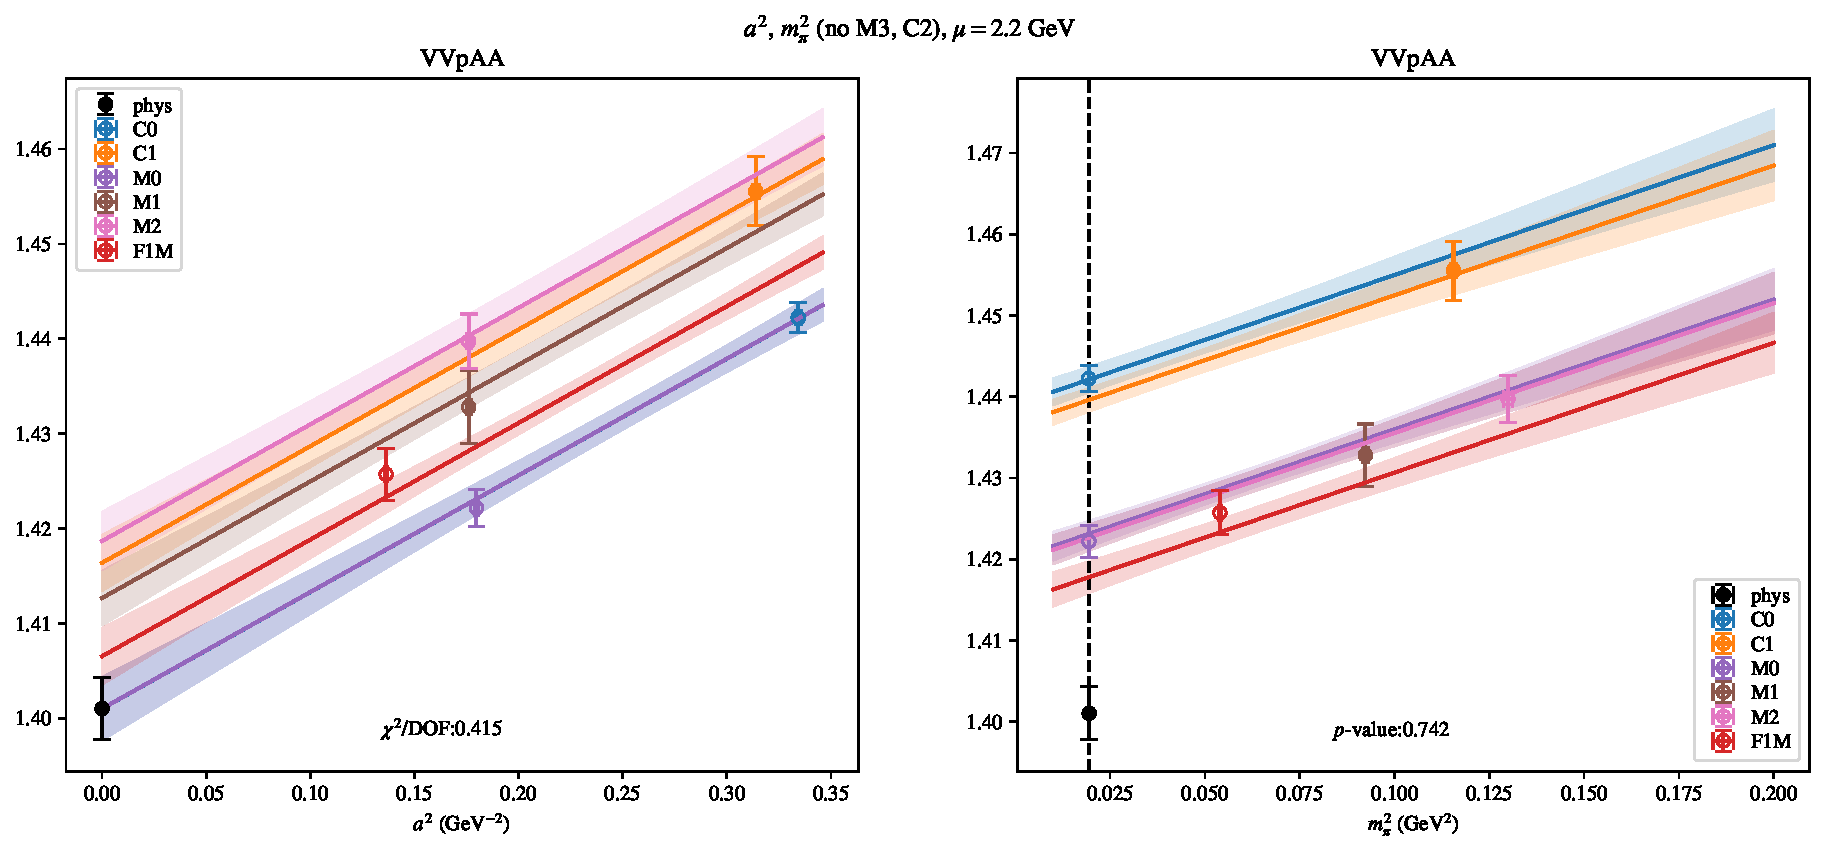
\includepdf[link, pages=-]{VVpAA/NPR/bag_a2m2mcut_22.pdf}
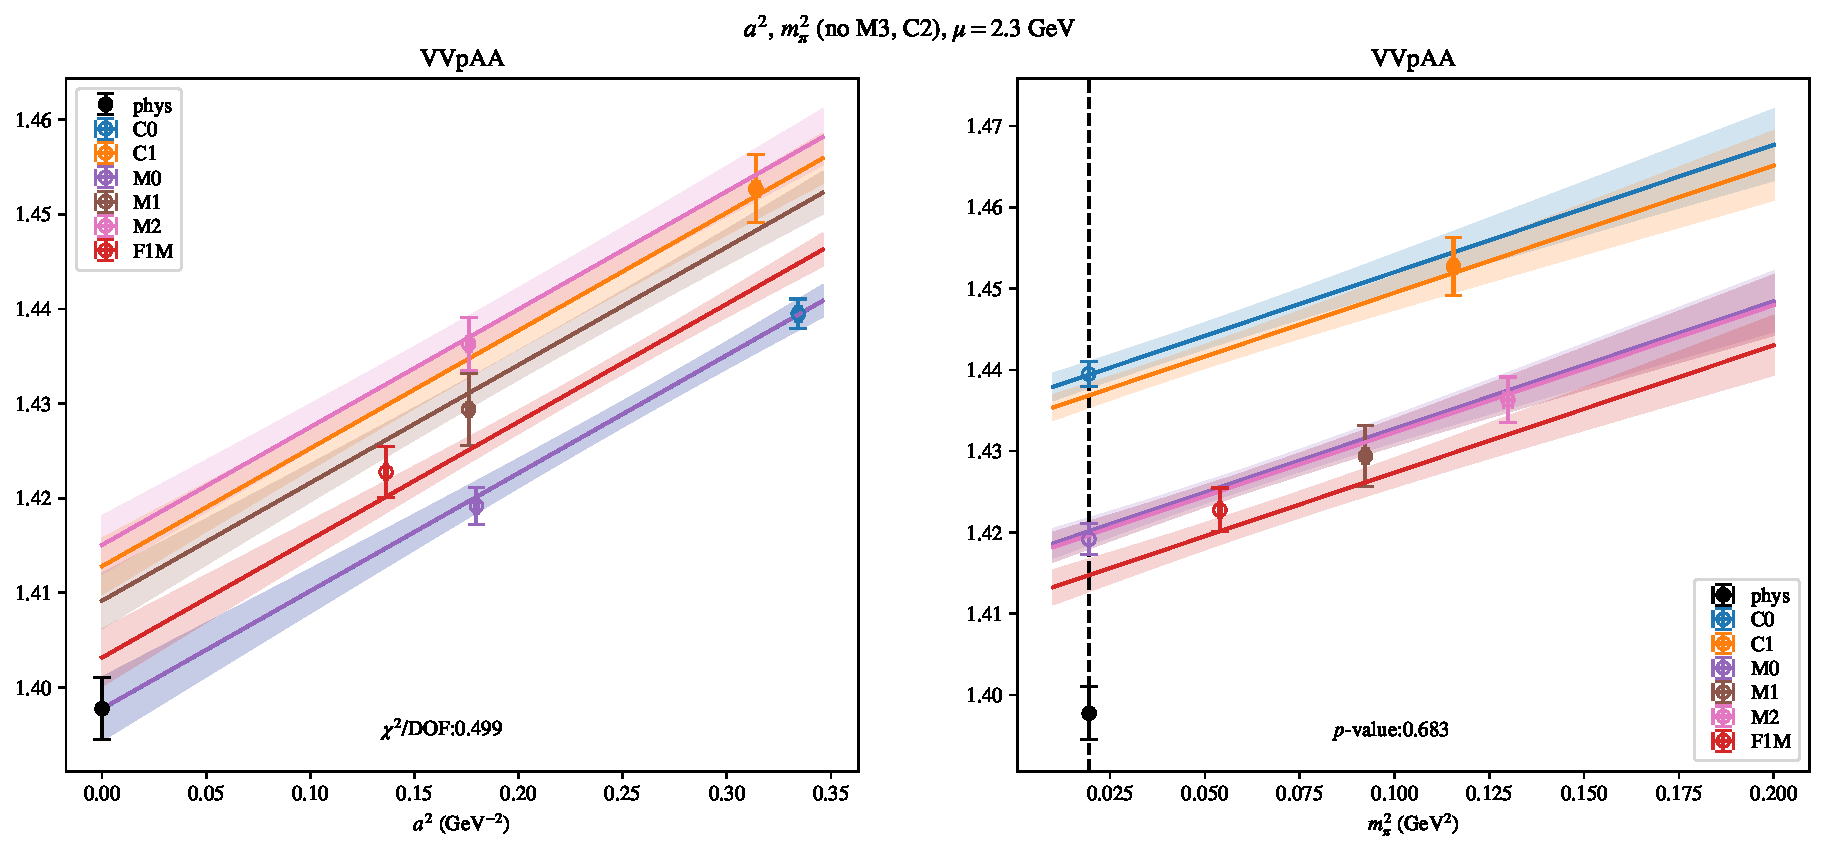
\includepdf[link, pages=-]{VVpAA/NPR/bag_a2m2mcut_23.pdf}
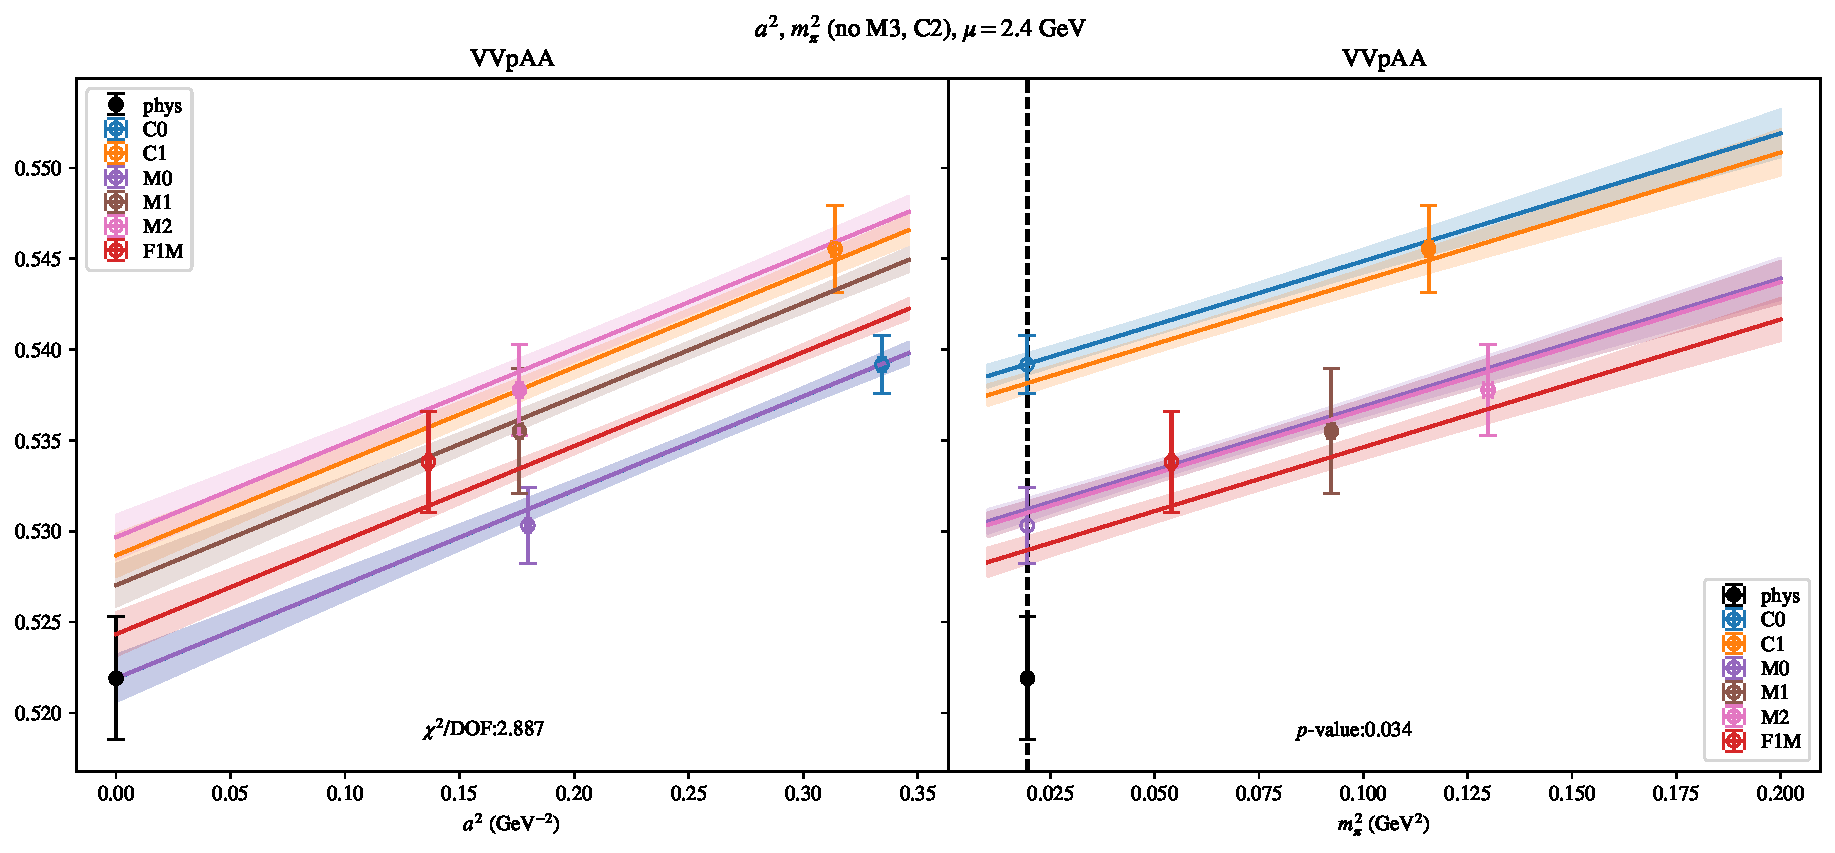
\includepdf[link, pages=-]{VVpAA/NPR/bag_a2m2mcut_24.pdf}
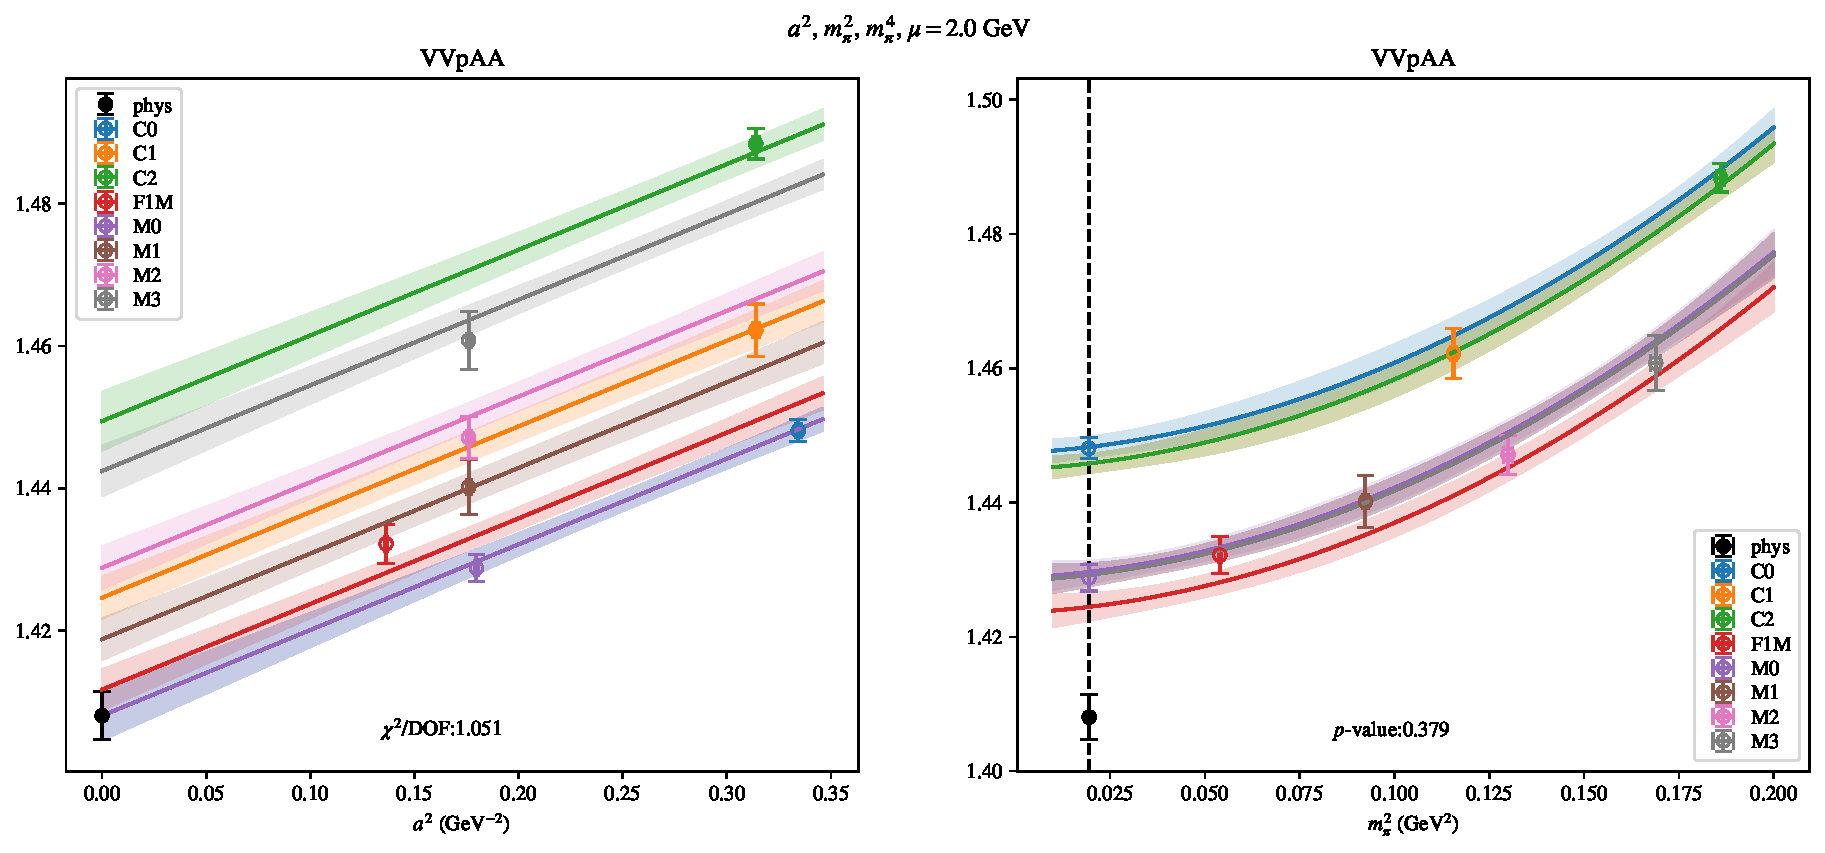
\includepdf[link, pages=-]{VVpAA/NPR/bag_a2m2m4_20.pdf}
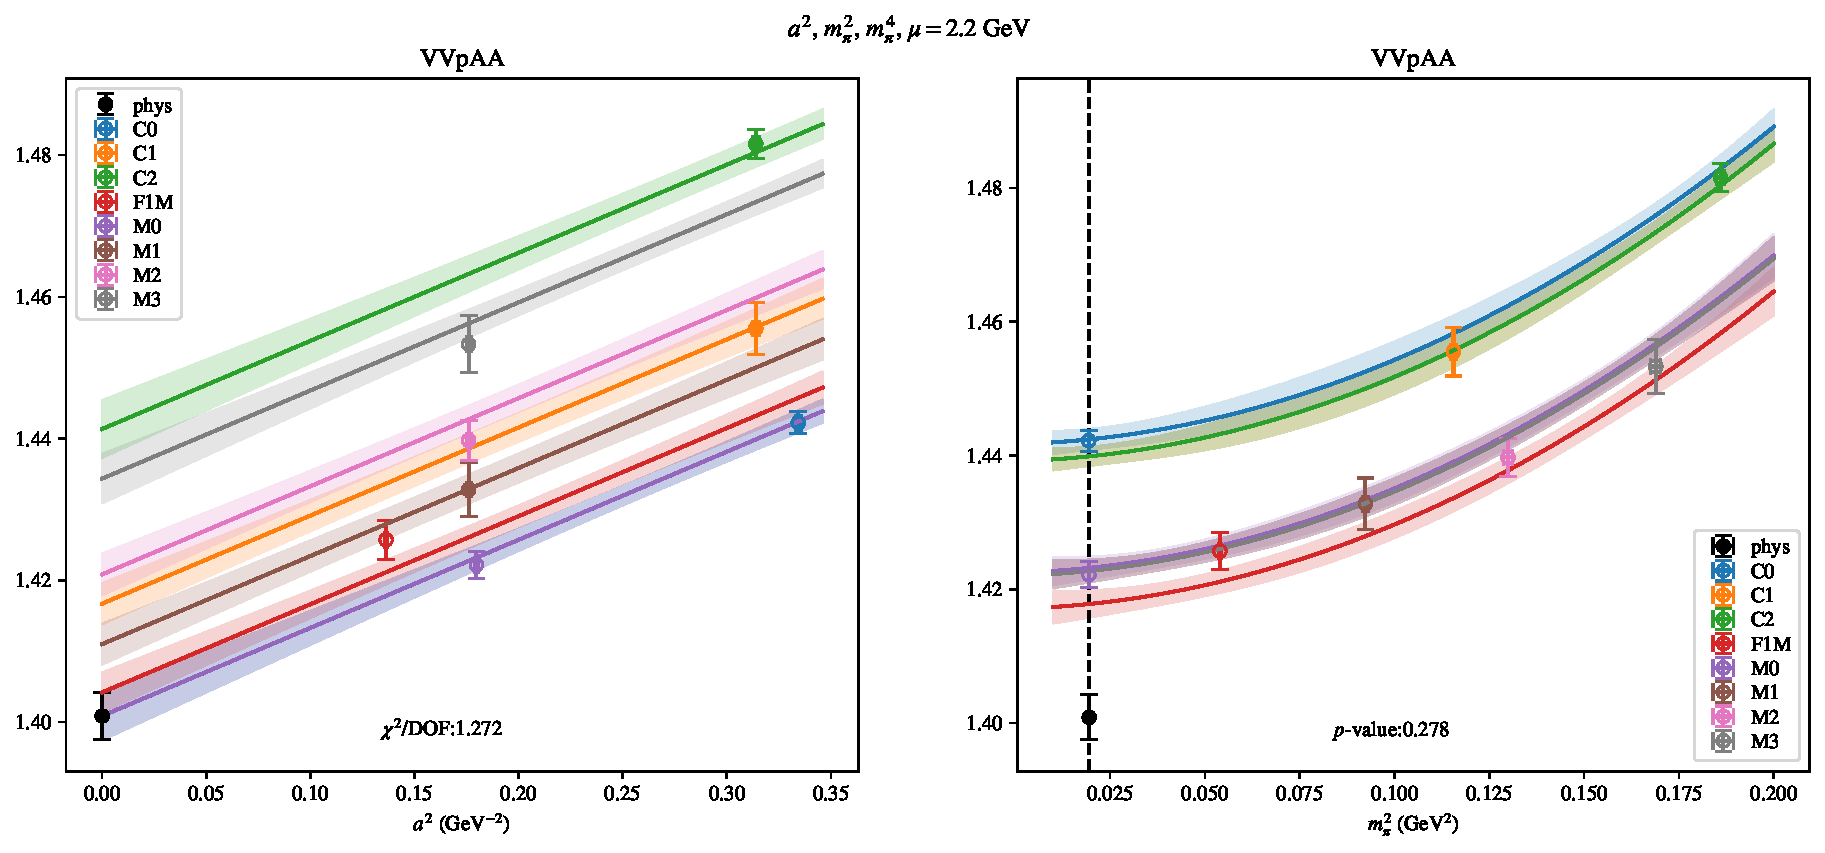
\includepdf[link, pages=-]{VVpAA/NPR/bag_a2m2m4_22.pdf}
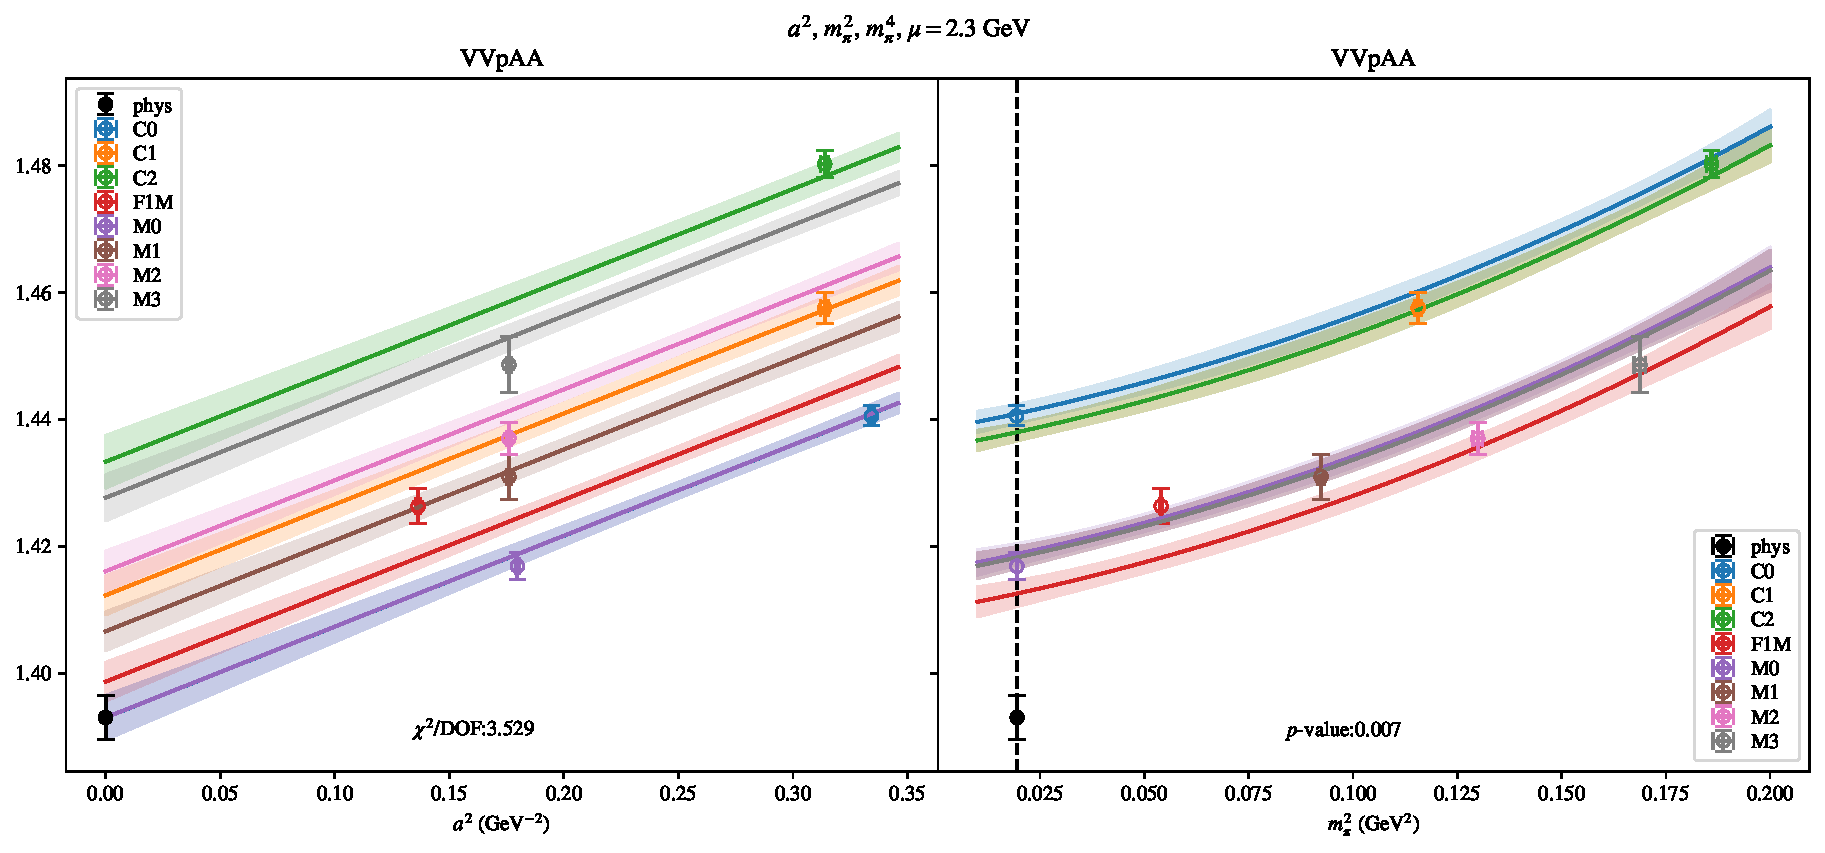
\includepdf[link, pages=-]{VVpAA/NPR/bag_a2m2m4_23.pdf}
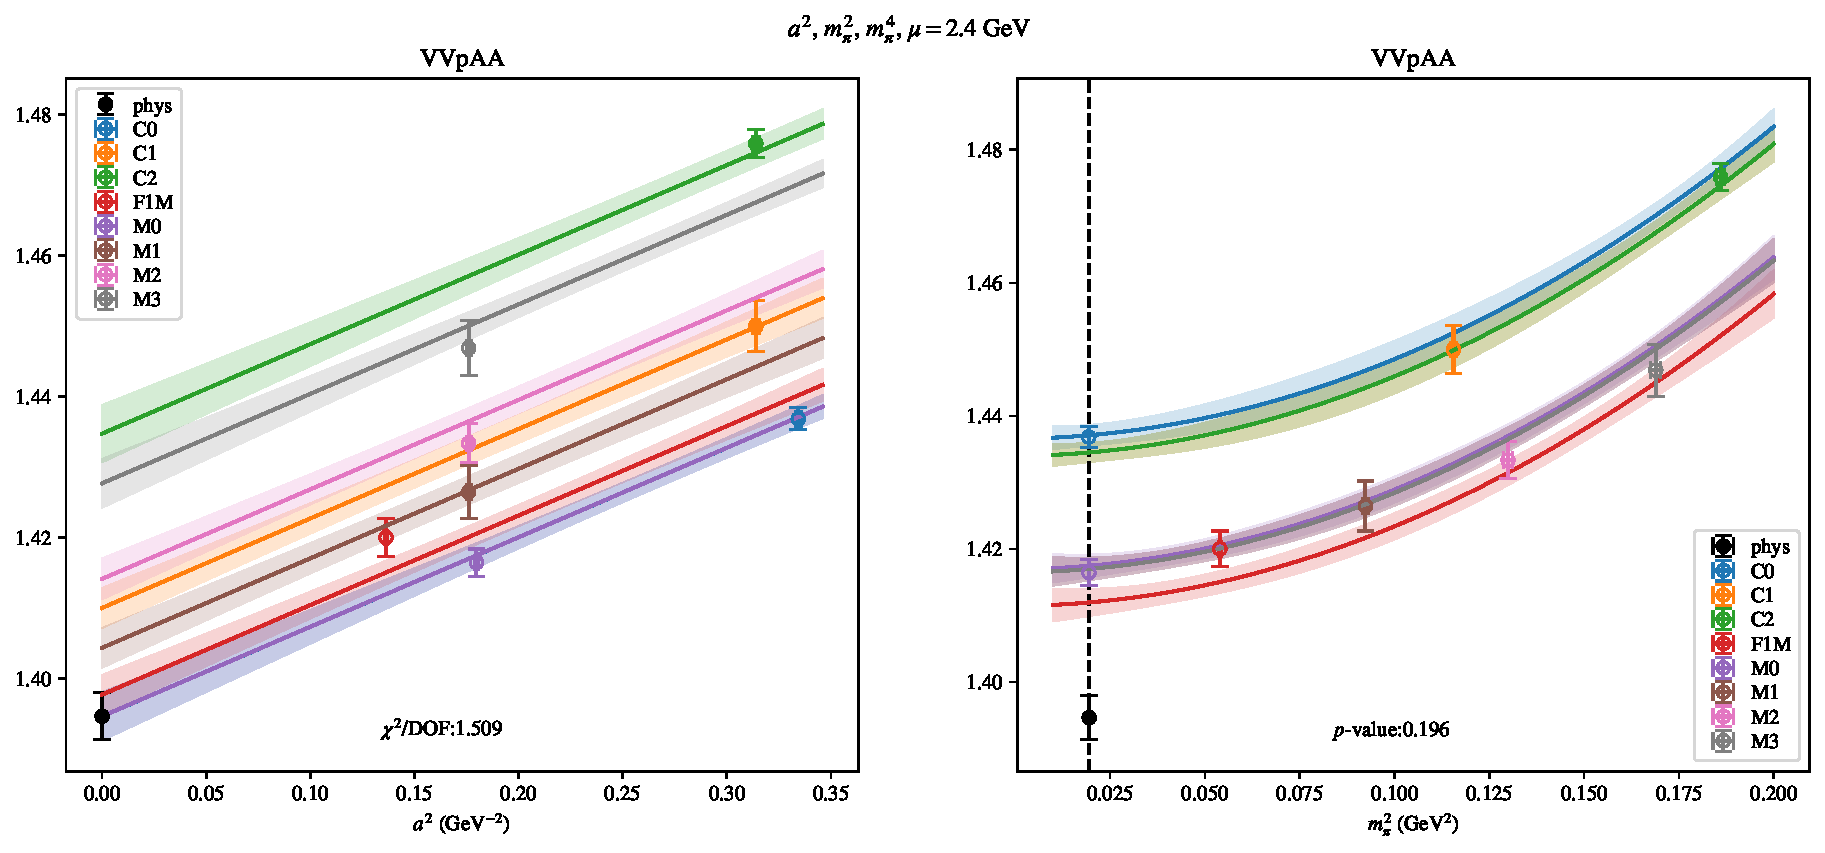
\includepdf[link, pages=-]{VVpAA/NPR/bag_a2m2m4_24.pdf}
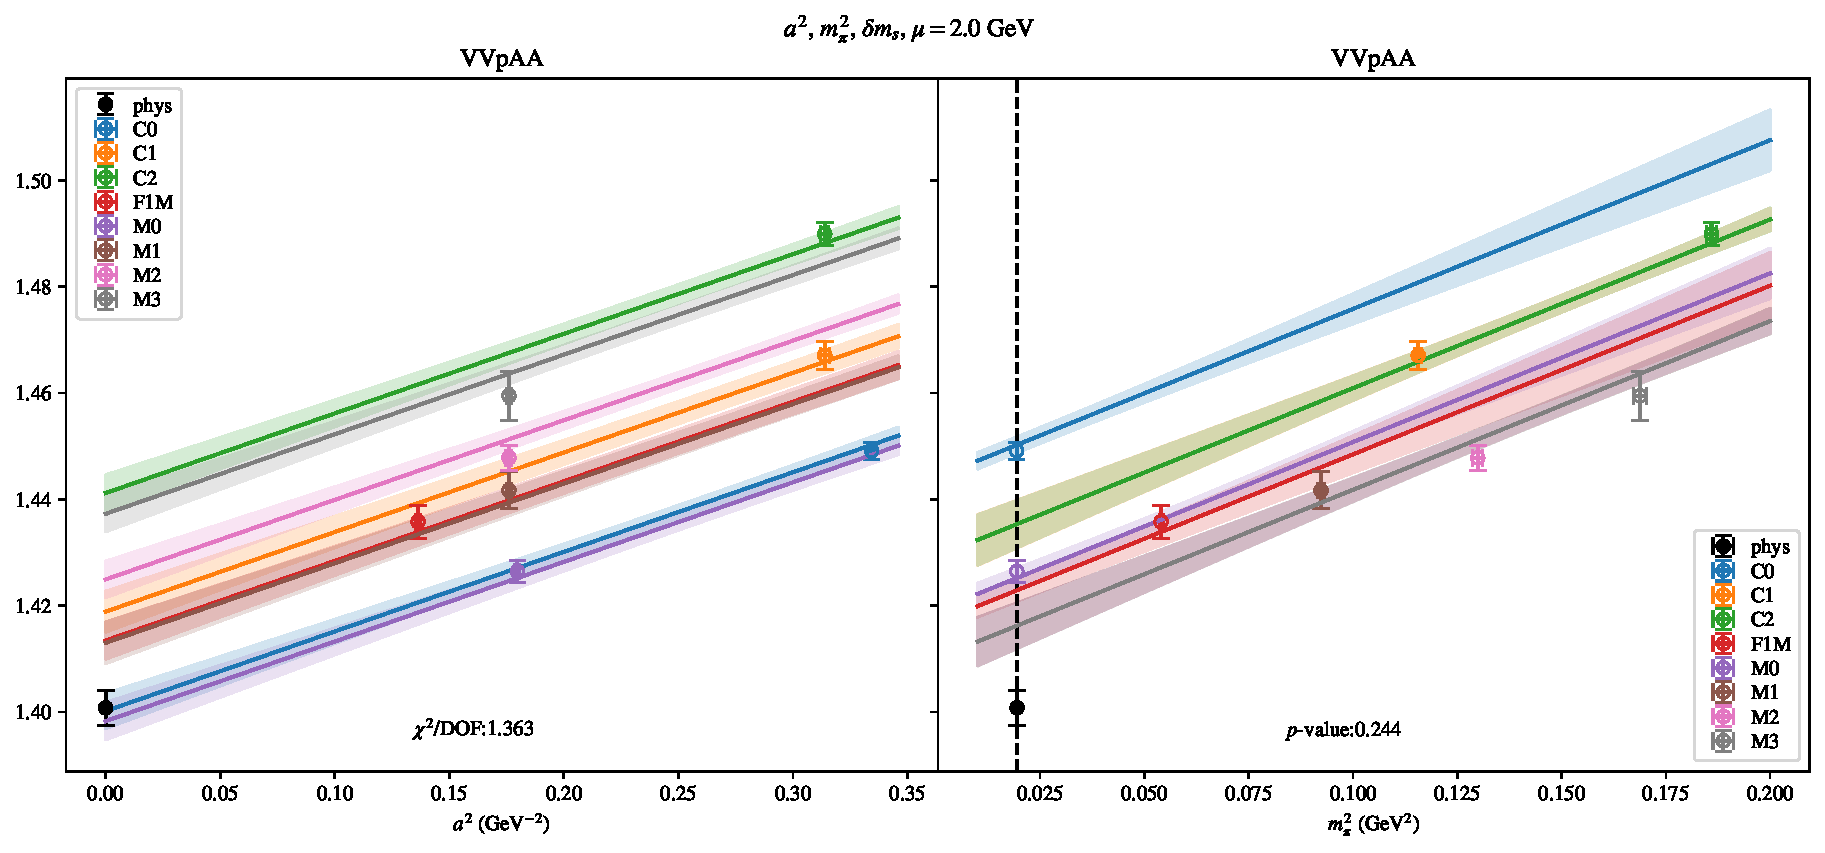
\includepdf[link, pages=-]{VVpAA/NPR/bag_a2m2delm_20.pdf}
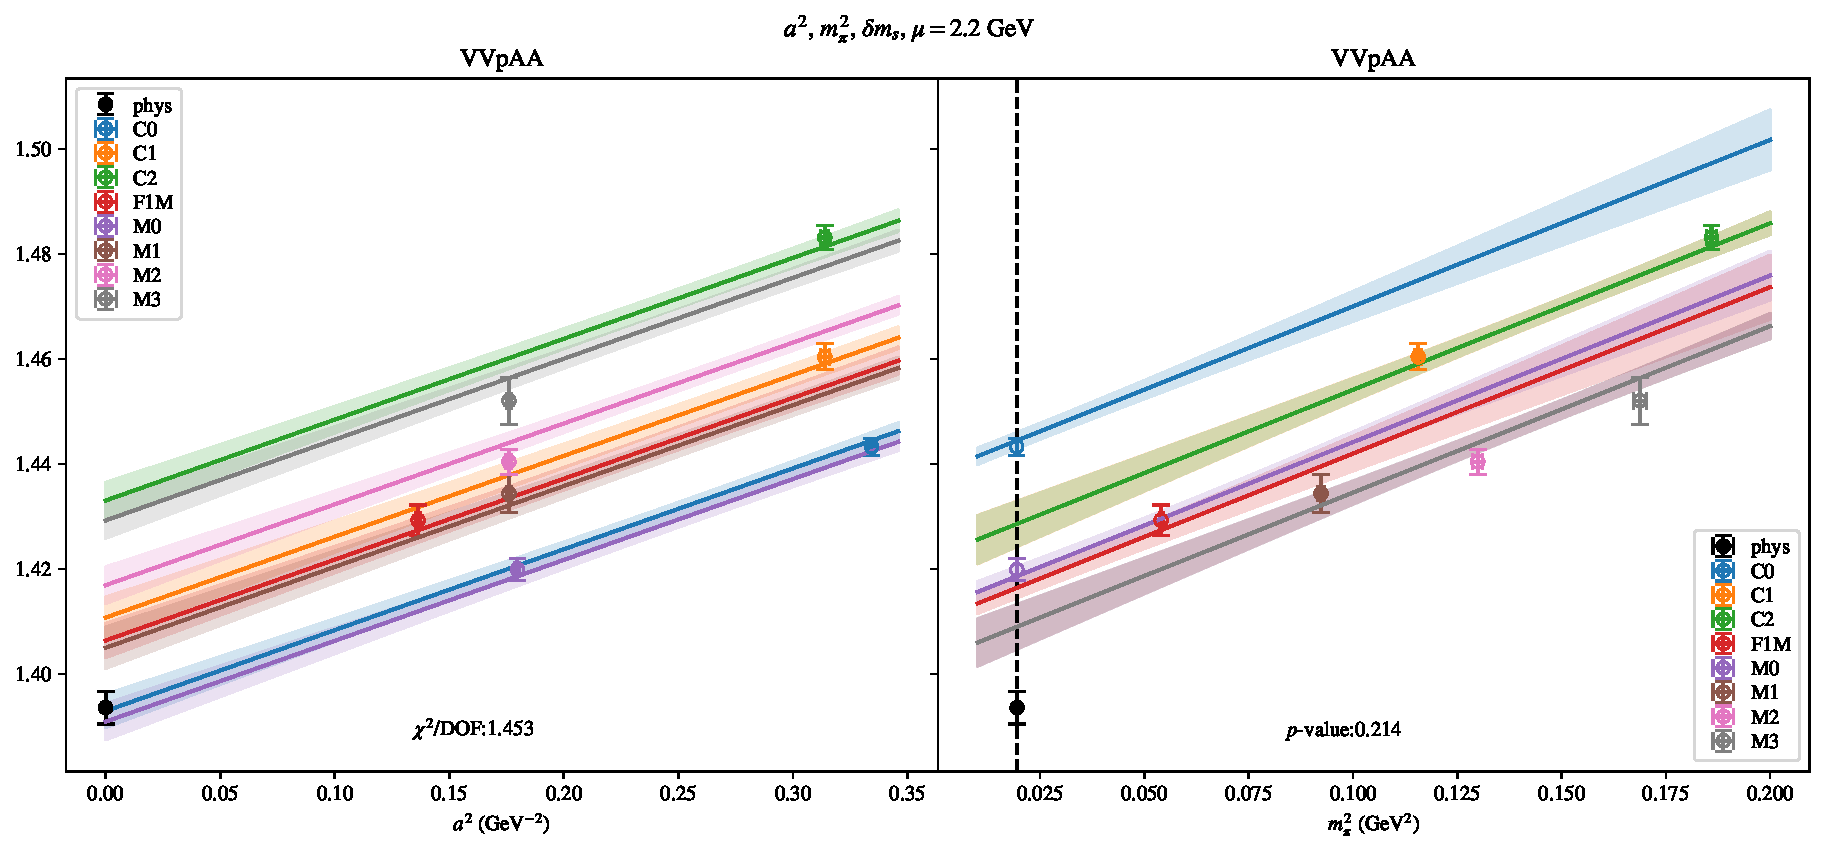
\includepdf[link, pages=-]{VVpAA/NPR/bag_a2m2delm_22.pdf}
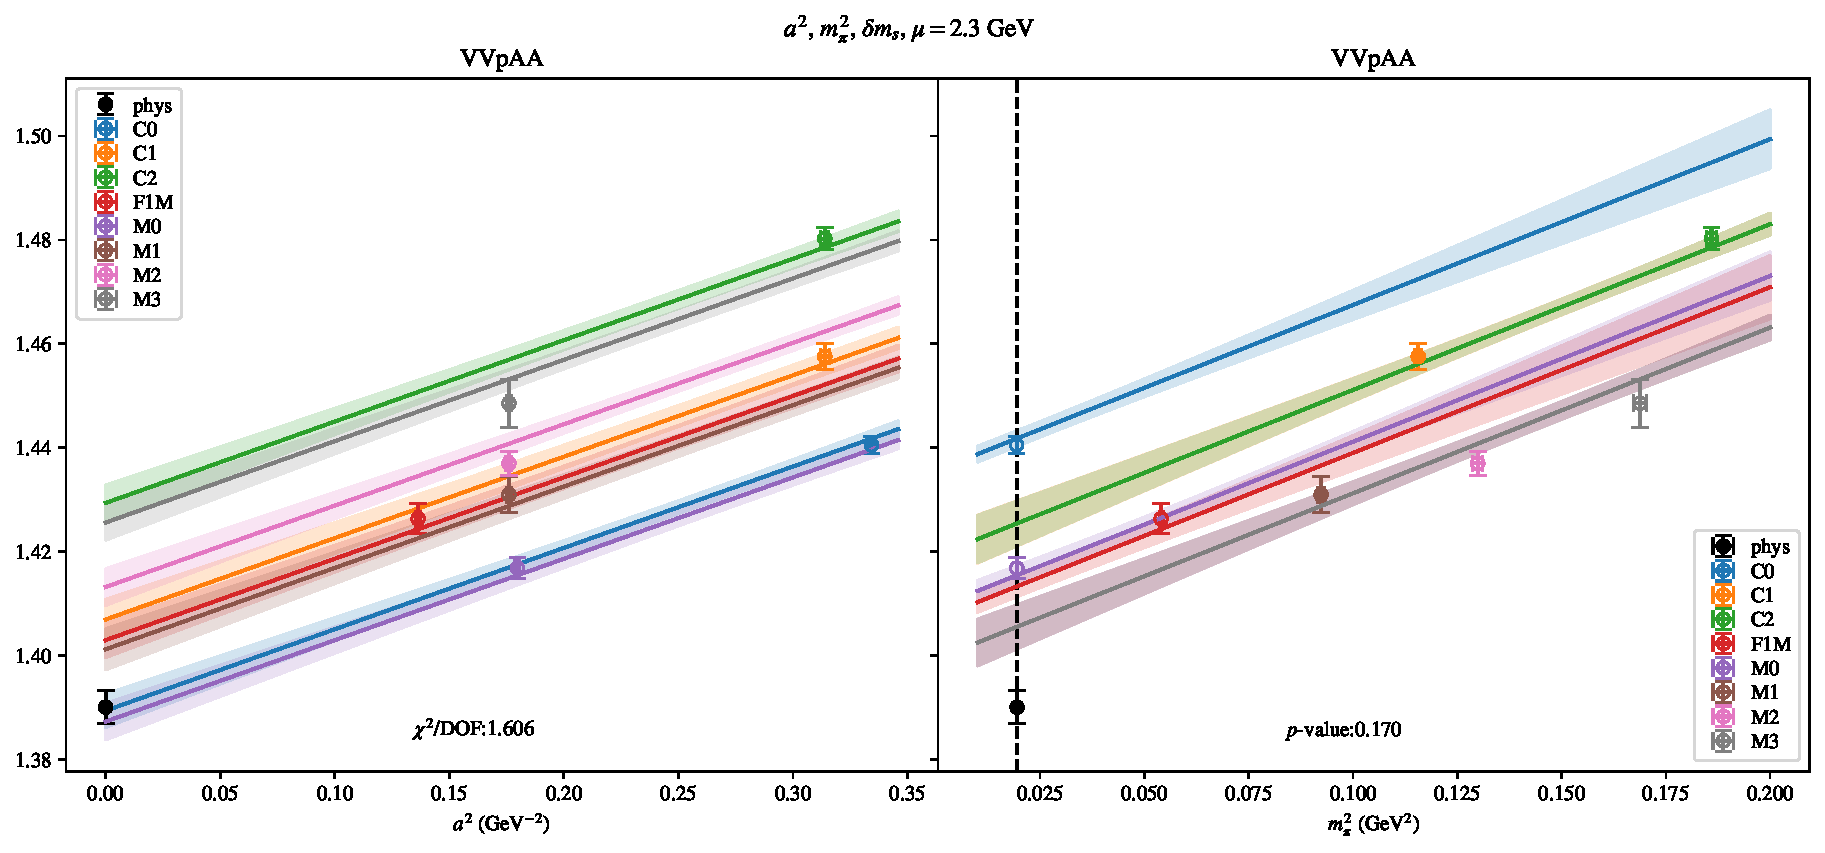
\includepdf[link, pages=-]{VVpAA/NPR/bag_a2m2delm_23.pdf}
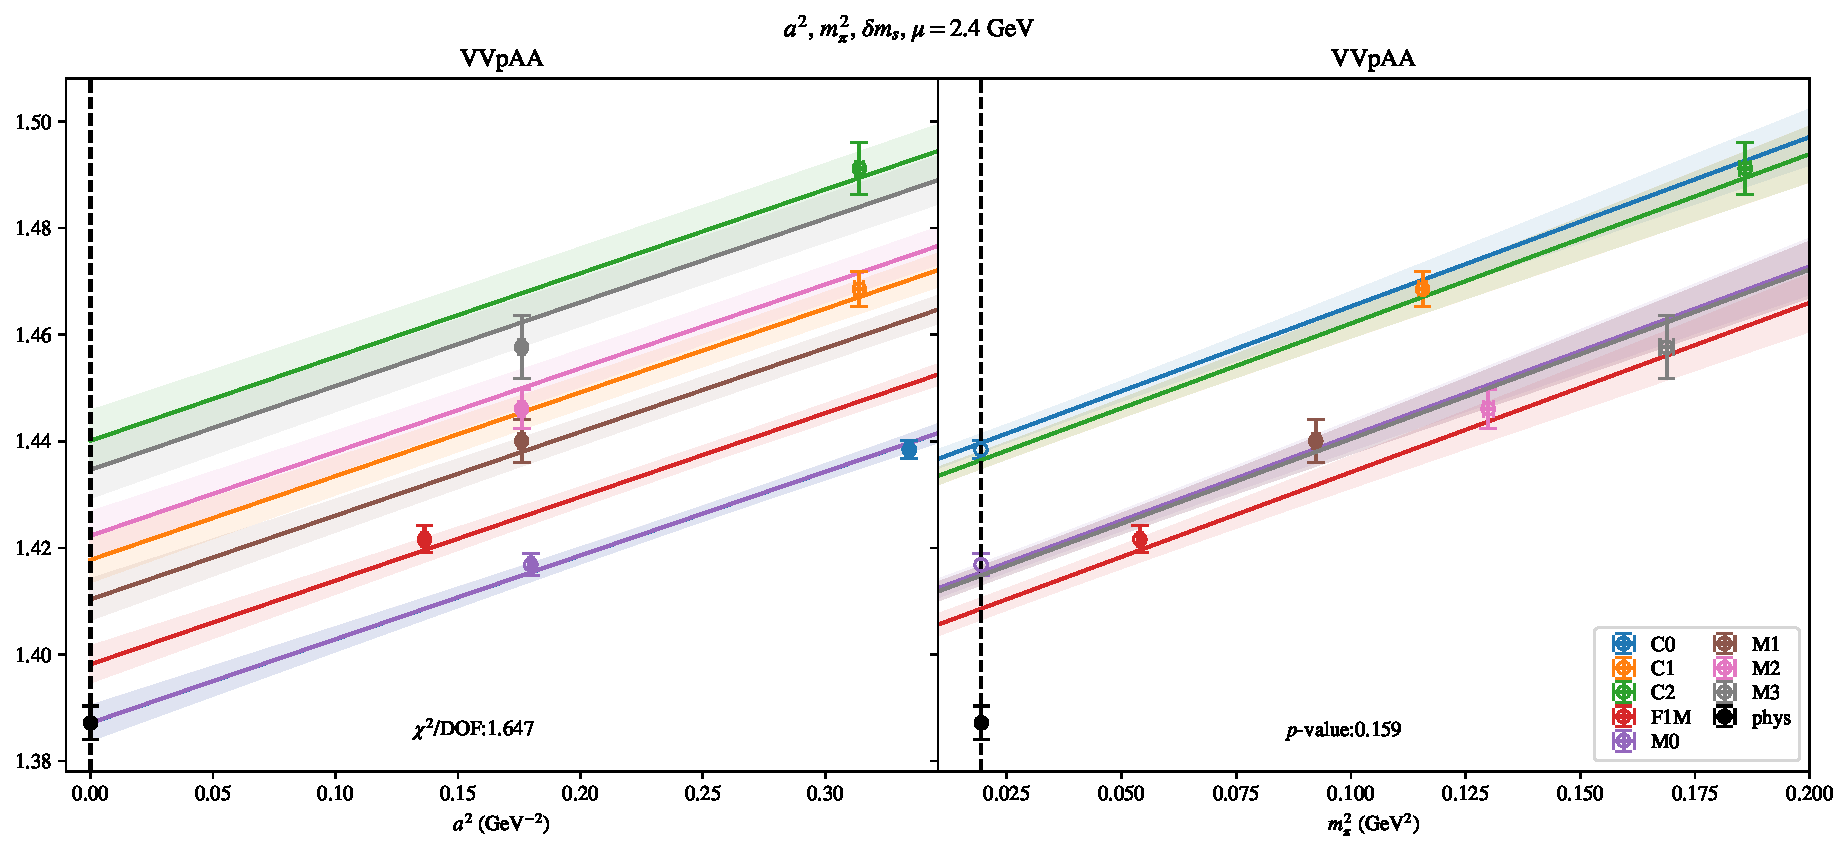
\includepdf[link, pages=-]{VVpAA/NPR/bag_a2m2delm_24.pdf}
\clearpage
\section{$\mathcal{B}_2$}
\begin{table}[h!]
\begin{center}
\begin{tabular}{|c|c|c|c|c|c|c|}
\hline
$\mu$ (GeV) & $a^2$, $m_\pi^2$& $a^2$, $m_\pi^2$ (no C)& $a^2$, $m_\pi^2$, $a^4$& $a^2$, $m_\pi^2$ (no M3, C2)& $a^2$, $m_\pi^2$, $m_\pi^4$& $a^2$, $m_\pi^2$, $\delta m_s$\\
\hline
2.0& \hyperlink{VVmAA/NPR/bag_a2m2_20.pdf.1}{\textbf{-0.9919(23)}: 10.034 (0.0)} & \hyperlink{VVmAA/NPR/bag_a2m2noC_20.pdf.1}{\textbf{-0.9259(95)}: 0.477 (0.621)} & \hyperlink{VVmAA/NPR/bag_a2a4m2_20.pdf.1}{\textbf{-0.889(13)}: 1.091 (0.359)} & \hyperlink{VVmAA/NPR/bag_a2m2mcut_20.pdf.1}{\textbf{-0.9925(21)}: 14.614 (0.0)} & \hyperlink{VVmAA/NPR/bag_a2m2m4_20.pdf.1}{\textbf{-0.9948(22)}: 8.074 (0.0)} & \hyperlink{VVmAA/NPR/bag_a2m2delm_20.pdf.1}{\textbf{-0.9965(24)}: 0.62 (0.649)}\\
2.2& \hyperlink{VVmAA/NPR/bag_a2m2_22.pdf.1}{\textbf{-1.0060(20)}: 8.915 (0.0)} & \hyperlink{VVmAA/NPR/bag_a2m2noC_22.pdf.1}{\textbf{-0.9489(89)}: 1.253 (0.286)} & \hyperlink{VVmAA/NPR/bag_a2a4m2_22.pdf.1}{\textbf{-0.915(13)}: 1.284 (0.274)} & \hyperlink{VVmAA/NPR/bag_a2m2mcut_22.pdf.1}{\textbf{-1.0066(19)}: 12.745 (0.0)} & \hyperlink{VVmAA/NPR/bag_a2m2m4_22.pdf.1}{\textbf{-1.0081(19)}: 7.225 (0.0)} & \hyperlink{VVmAA/NPR/bag_a2m2delm_22.pdf.1}{\textbf{-1.0092(21)}: 1.455 (0.213)}\\
2.3& \hyperlink{VVmAA/NPR/bag_a2m2_23.pdf.1}{\textbf{-1.0119(18)}: 9.373 (0.0)} & \hyperlink{VVmAA/NPR/bag_a2m2noC_23.pdf.1}{\textbf{-0.9563(88)}: 1.66 (0.19)} & \hyperlink{VVmAA/NPR/bag_a2a4m2_23.pdf.1}{\textbf{-0.922(13)}: 1.321 (0.259)} & \hyperlink{VVmAA/NPR/bag_a2m2mcut_23.pdf.1}{\textbf{-1.0125(17)}: 13.608 (0.0)} & \hyperlink{VVmAA/NPR/bag_a2m2m4_23.pdf.1}{\textbf{-1.0140(17)}: 7.826 (0.0)} & \hyperlink{VVmAA/NPR/bag_a2m2delm_23.pdf.1}{\textbf{-1.0148(19)}: 1.86 (0.114)}\\
2.4& \hyperlink{VVmAA/NPR/bag_a2m2_24.pdf.1}{\textbf{-1.0168(17)}: 9.097 (0.0)} & \hyperlink{VVmAA/NPR/bag_a2m2noC_24.pdf.1}{\textbf{-0.9633(86)}: 1.942 (0.143)} & \hyperlink{VVmAA/NPR/bag_a2a4m2_24.pdf.1}{\textbf{-0.932(12)}: 1.575 (0.178)} & \hyperlink{VVmAA/NPR/bag_a2m2mcut_24.pdf.1}{\textbf{-1.0173(16)}: 13.168 (0.0)} & \hyperlink{VVmAA/NPR/bag_a2m2m4_24.pdf.1}{\textbf{-1.0187(16)}: 7.737 (0.0)} & \hyperlink{VVmAA/NPR/bag_a2m2delm_24.pdf.1}{\textbf{-1.0193(18)}: 2.072 (0.082)}\\
\hline
\end{tabular}
\caption{Physical point value from chiral and continuum extrapolation at renormalisation scale $\mu$. Entries are \textbf{value(error)}: $\chi^2/\text{DOF}$ ($p$-value).}
\end{center}
\end{table}
\begin{table}[h!]
\begin{center}
\begin{tabular}{|c c|c|c|c|c|c|c|}
\hline
$\mu$ (GeV) &  & $a^2$, $m_\pi^2$& $a^2$, $m_\pi^2$ (no C)& $a^2$, $m_\pi^2$, $a^4$& $a^2$, $m_\pi^2$ (no M3, C2)& $a^2$, $m_\pi^2$, $m_\pi^4$& $a^2$, $m_\pi^2$, $\delta m_s$\\
\hline
\multirow{3}{0.5in}{2.0} & $\alpha$ & 0.1796(81)& -0.201(55)& -0.74(11)& 0.1813(74)& 0.1892(78)& 0.1958(87)\\
 & $\beta$ & -0.00161(27)& -0.00203(52)& -0.00145(27)& -0.00085(39)& 0.00319(85)& -0.00137(27)\\
 & $\gamma$ &  &  & 1.83(23)&  & -0.000454(68)& -0.0164(22)\\
\hline
\multirow{3}{0.5in}{2.2} & $\alpha$ & 0.2247(72)& -0.104(51)& -0.58(11)& 0.2263(66)& 0.2313(69)& 0.2365(75)\\
 & $\beta$ & -0.00134(18)& -0.00138(43)& -0.00108(19)& -0.00072(29)& 0.00214(74)& -0.00107(19)\\
 & $\gamma$ &  &  & 1.60(23)&  & -0.000323(62)& -0.0142(21)\\
\hline
\multirow{3}{0.5in}{2.3} & $\alpha$ & 0.2471(65)& -0.074(50)& -0.55(11)& 0.2488(61)& 0.2536(63)& 0.2576(69)\\
 & $\beta$ & -0.00146(17)& -0.00143(34)& -0.00121(17)& -0.00091(27)& 0.00173(70)& -0.00117(17)\\
 & $\gamma$ &  &  & 1.59(23)&  & -0.000297(60)& -0.0137(21)\\
\hline
\multirow{3}{0.5in}{2.4} & $\alpha$ & 0.2684(62)& -0.039(49)& -0.48(11)& 0.2698(58)& 0.2745(61)& 0.2778(65)\\
 & $\beta$ & -0.00145(15)& -0.00144(29)& -0.00121(16)& -0.00096(25)& 0.00139(66)& -0.00116(16)\\
 & $\gamma$ &  &  & 1.50(22)&  & -0.000263(57)& -0.0130(20)\\
\hline
\end{tabular}
\caption{Fit values of coefficients in $Q = Q_{phys} + \mathbf{\alpha} a^2 + \mathbf{\beta}\left(\frac{m_\pi^2}{f_\pi^2}-\frac{m_{\pi,PDG}^2}{f_\pi^2}\right) + \gamma(\ldots)$}
\end{center}
\end{table}
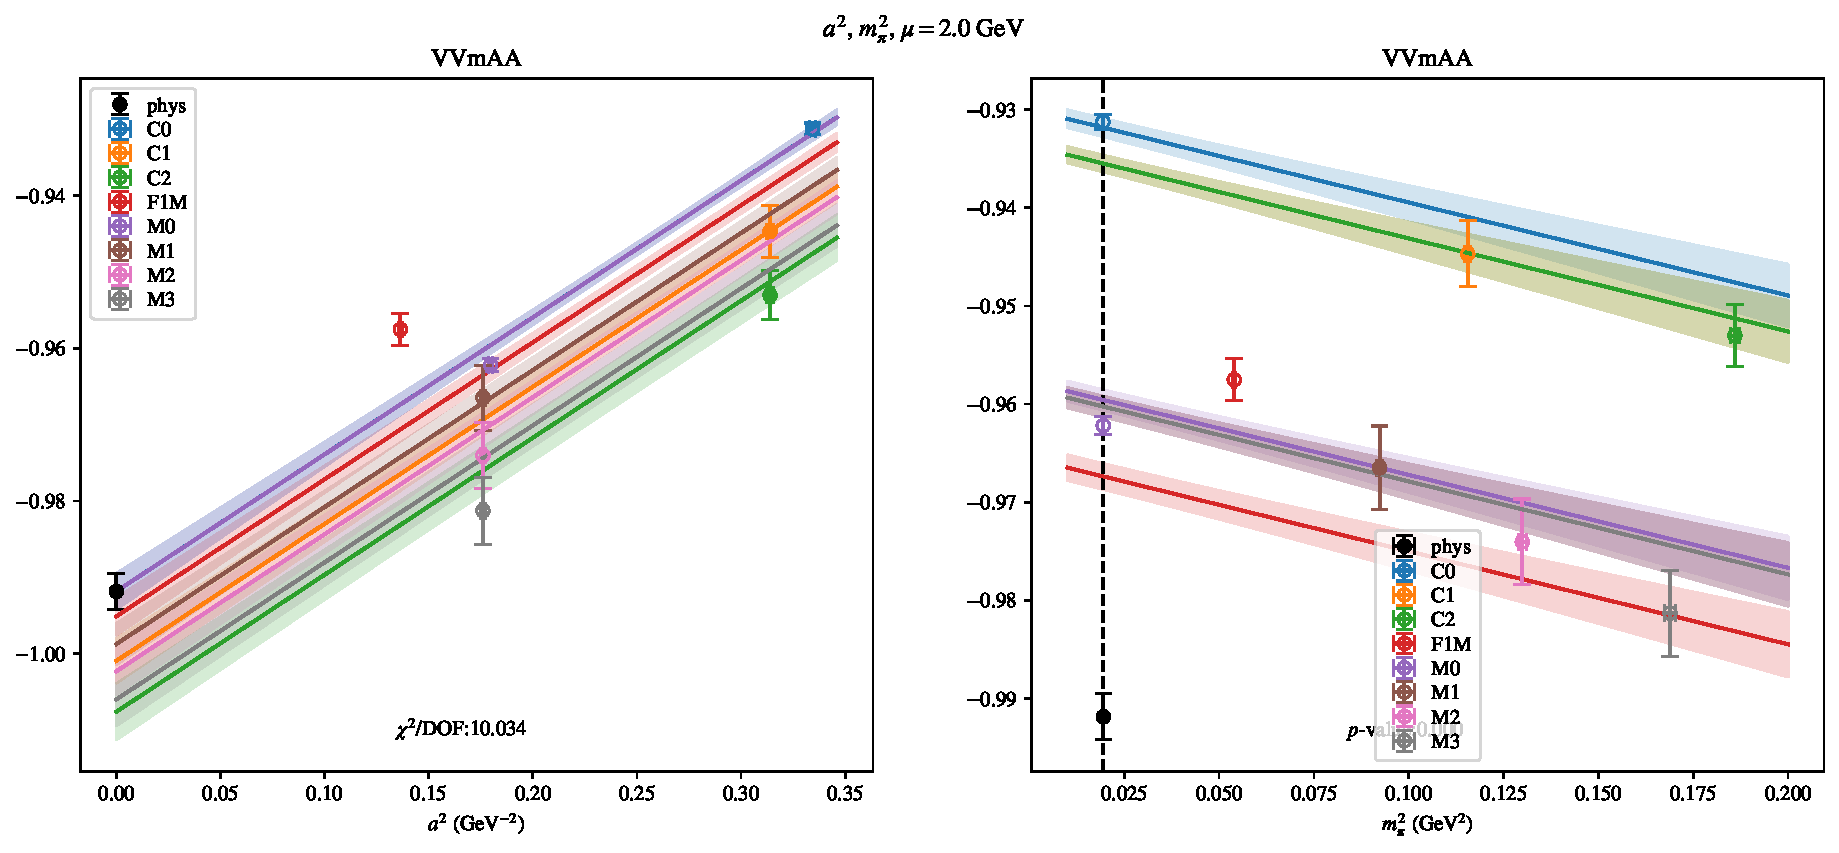
\includepdf[link, pages=-]{VVmAA/NPR/bag_a2m2_20.pdf}
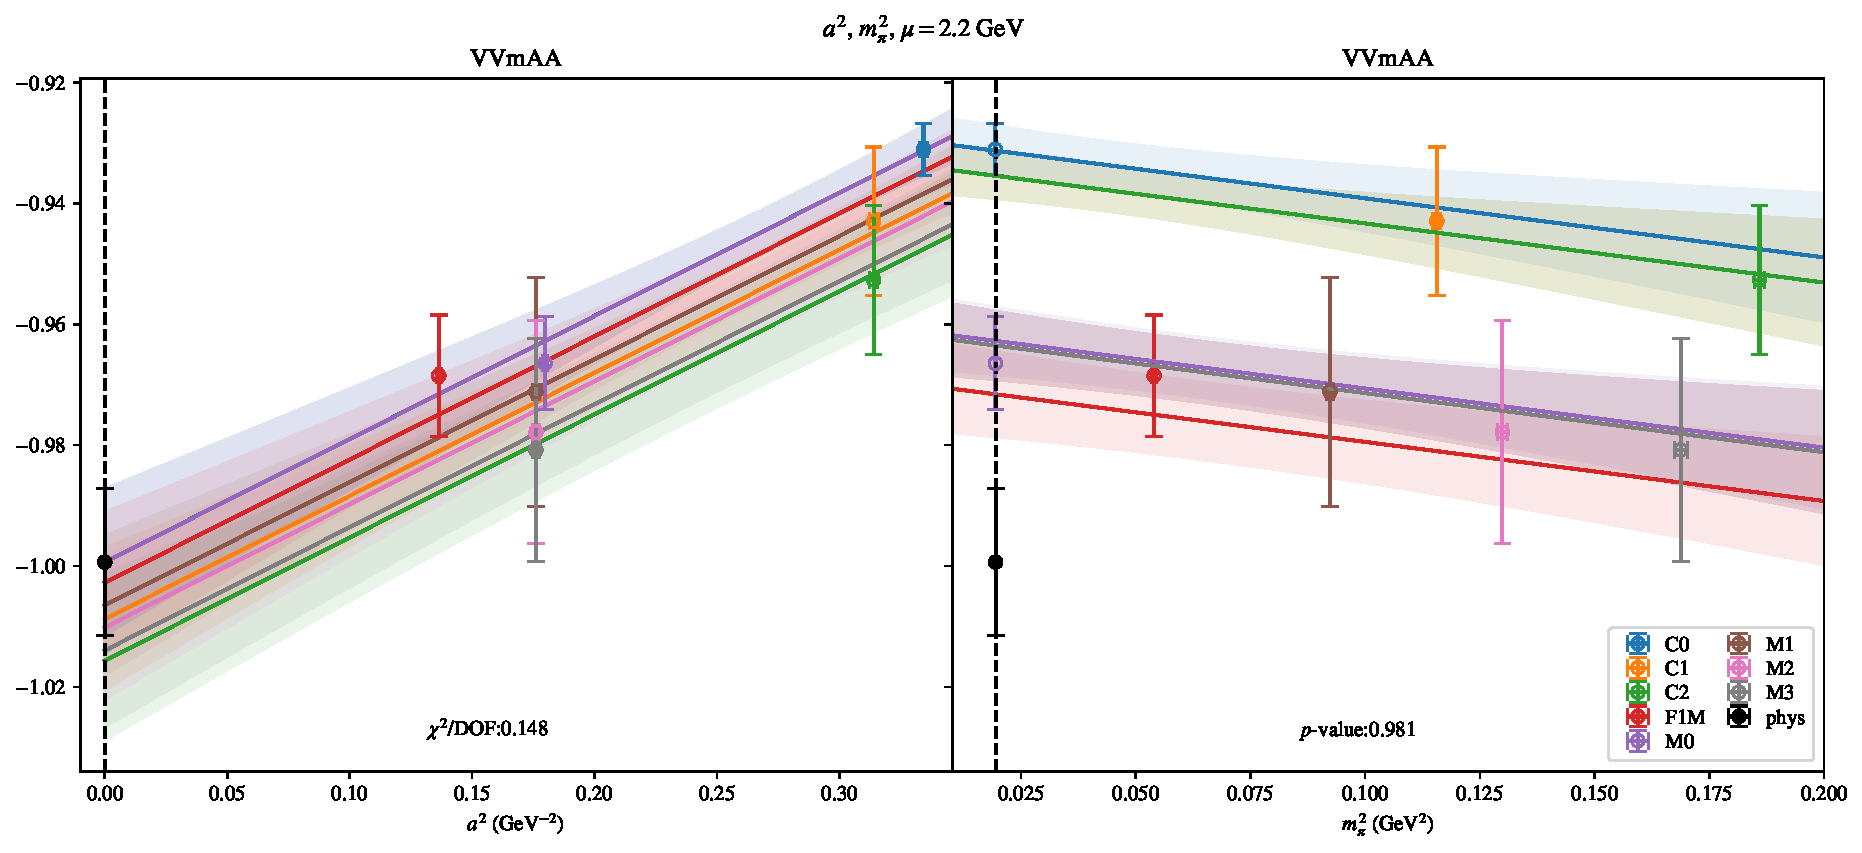
\includepdf[link, pages=-]{VVmAA/NPR/bag_a2m2_22.pdf}
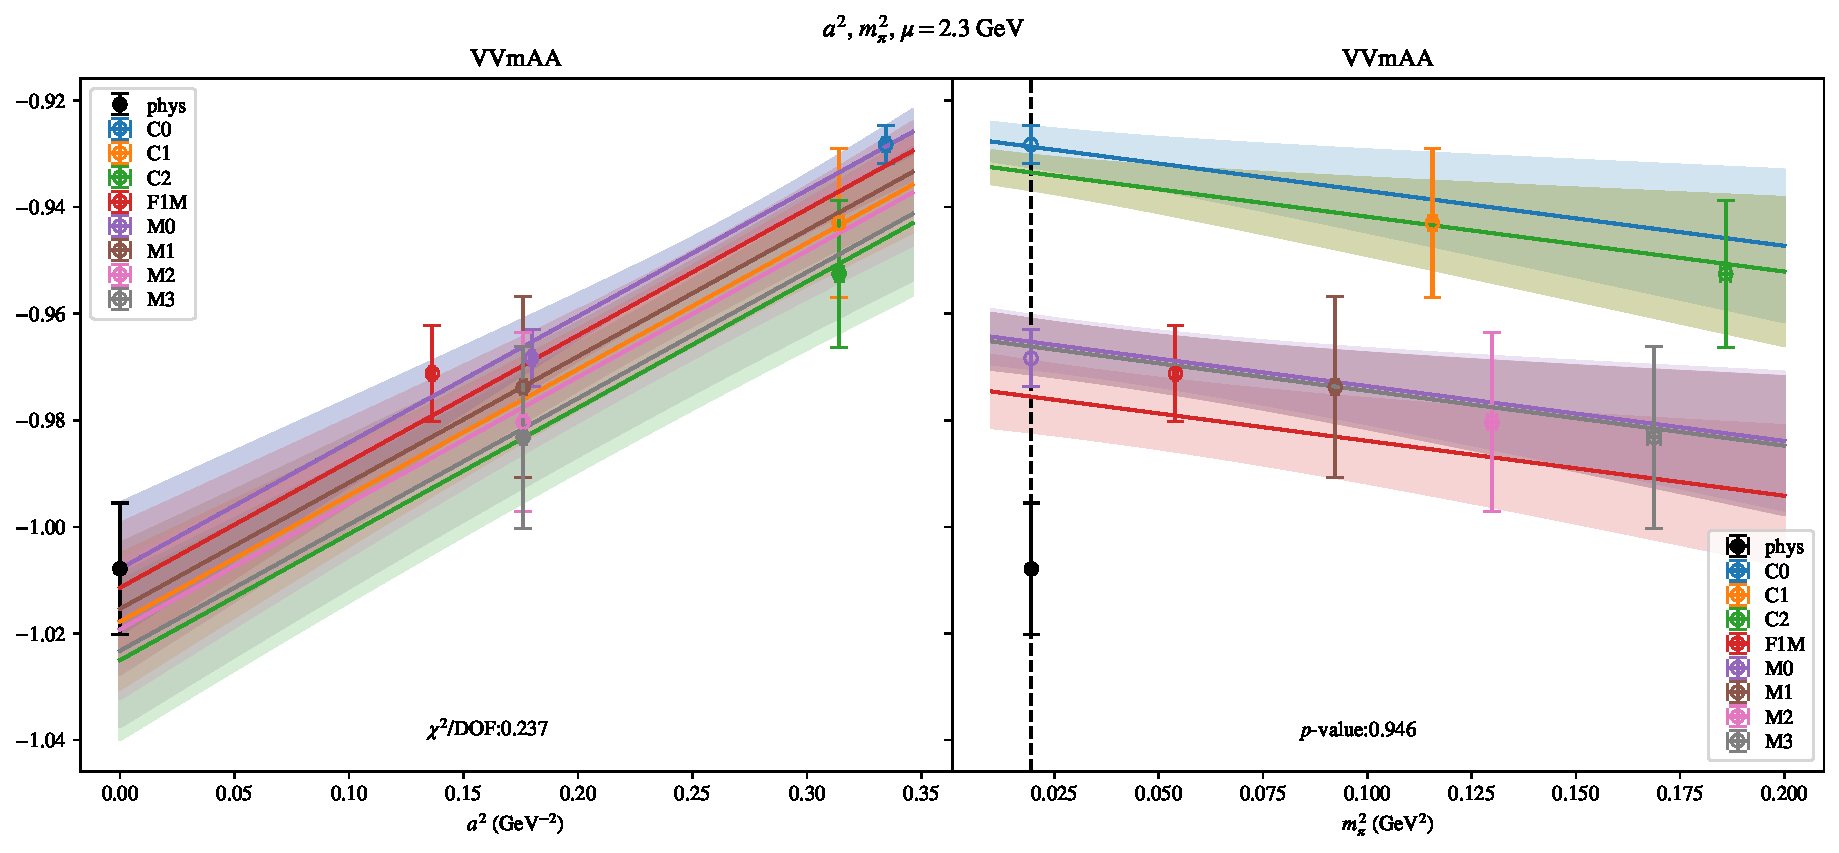
\includepdf[link, pages=-]{VVmAA/NPR/bag_a2m2_23.pdf}
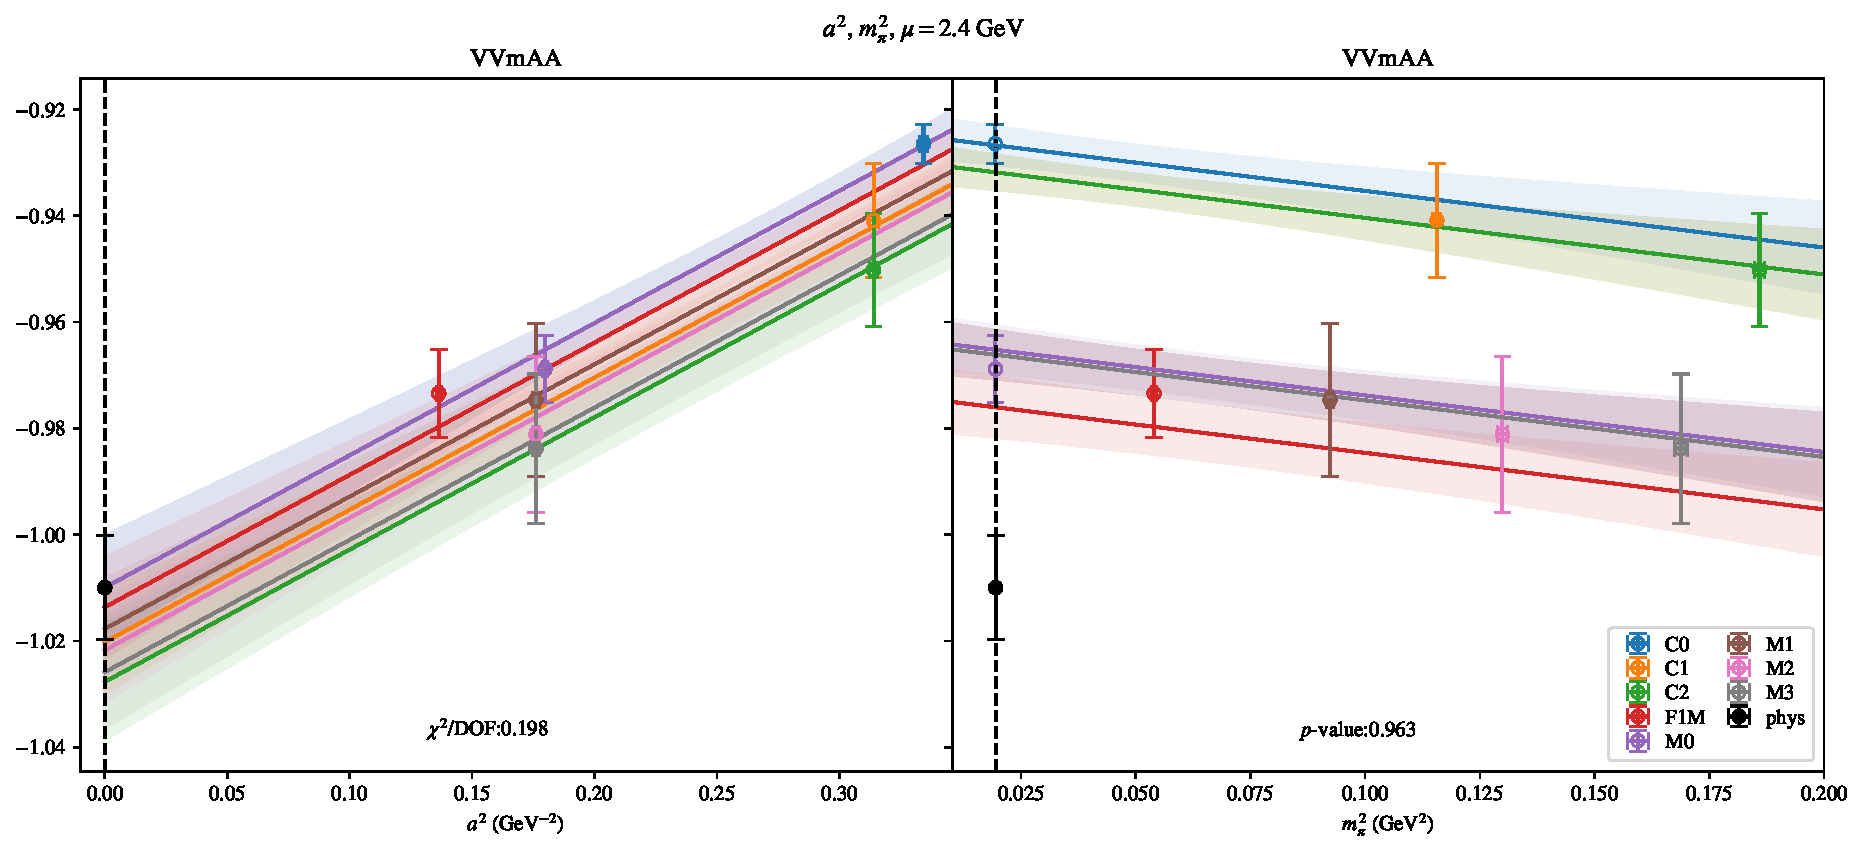
\includepdf[link, pages=-]{VVmAA/NPR/bag_a2m2_24.pdf}
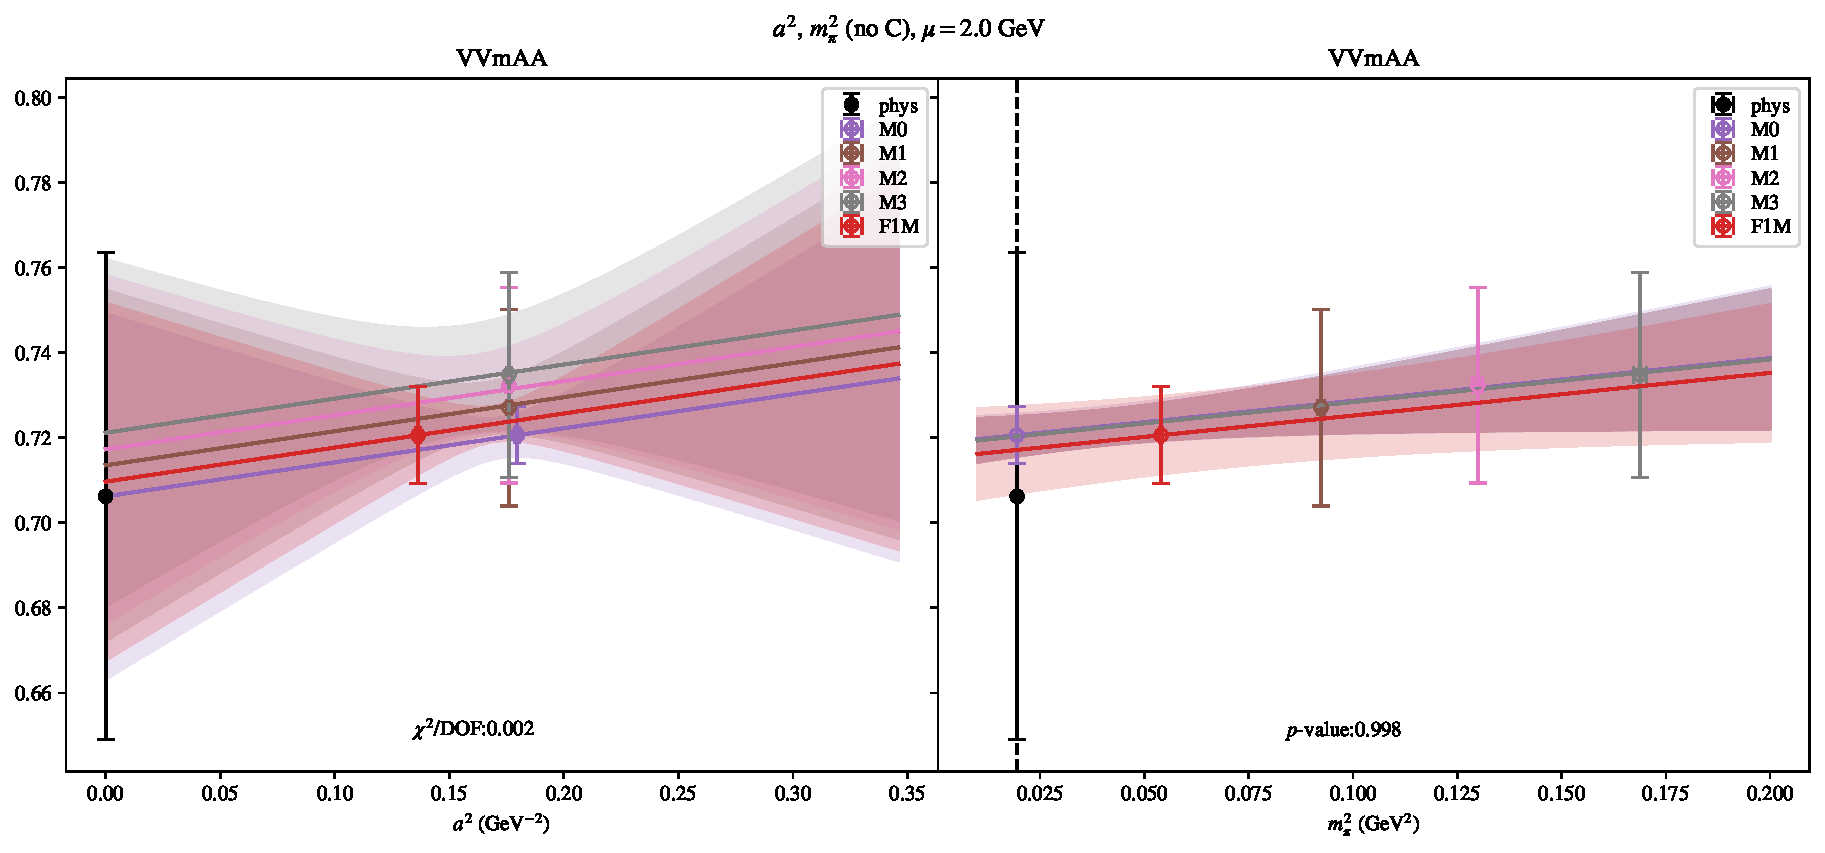
\includepdf[link, pages=-]{VVmAA/NPR/bag_a2m2noC_20.pdf}
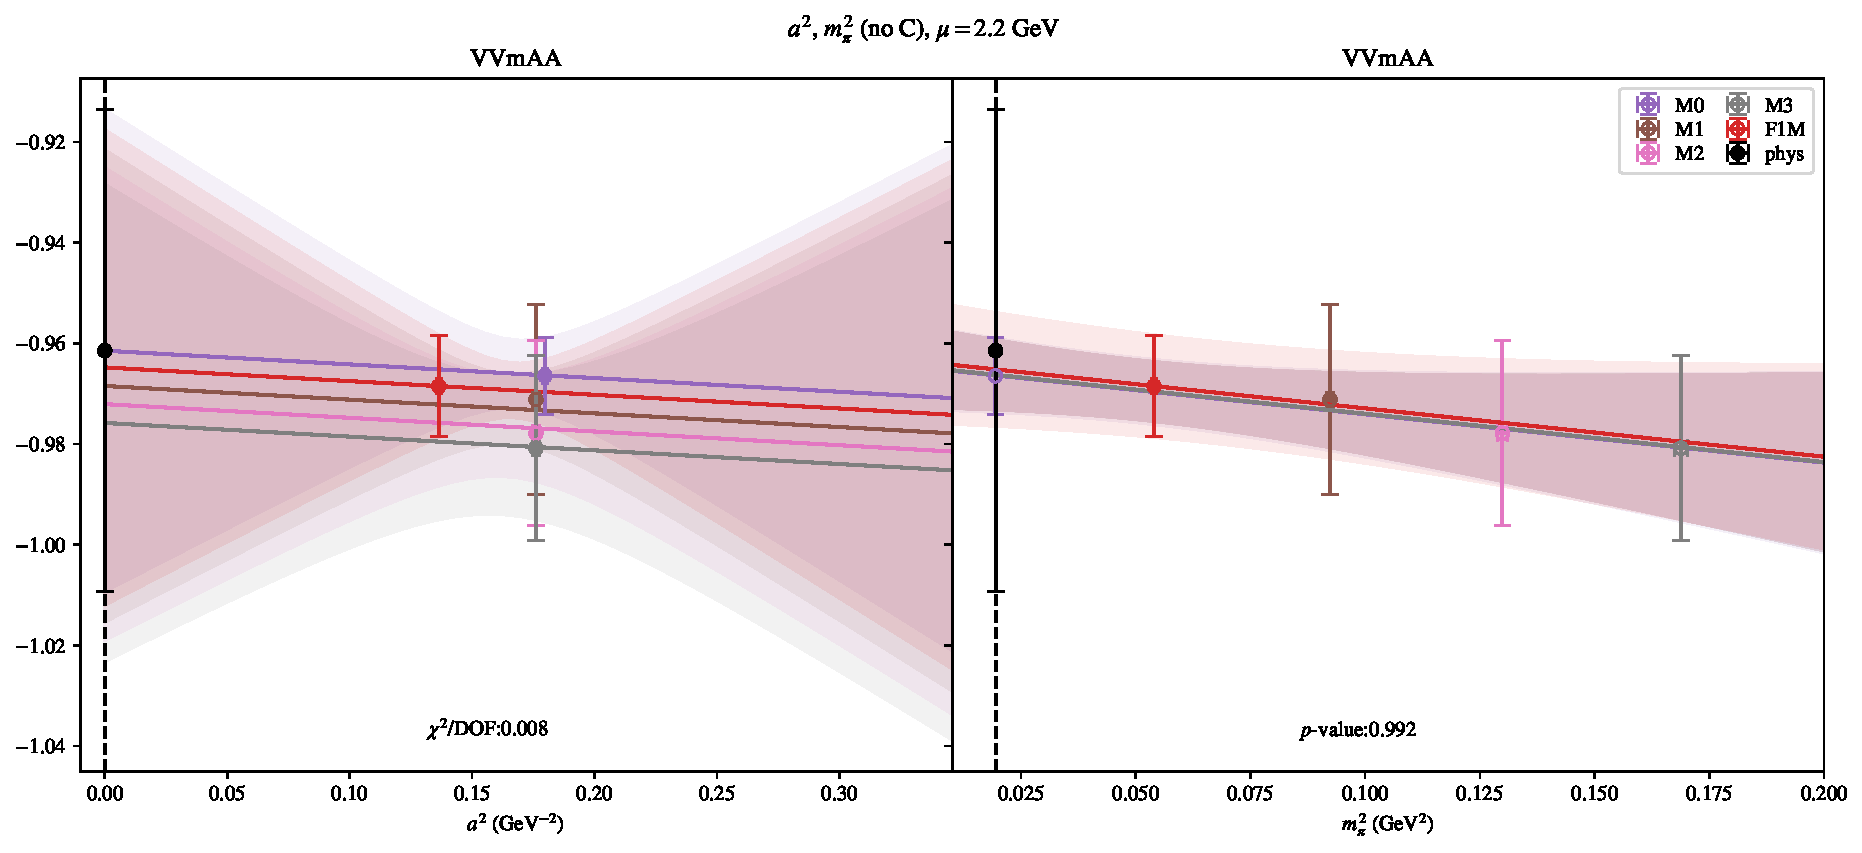
\includepdf[link, pages=-]{VVmAA/NPR/bag_a2m2noC_22.pdf}
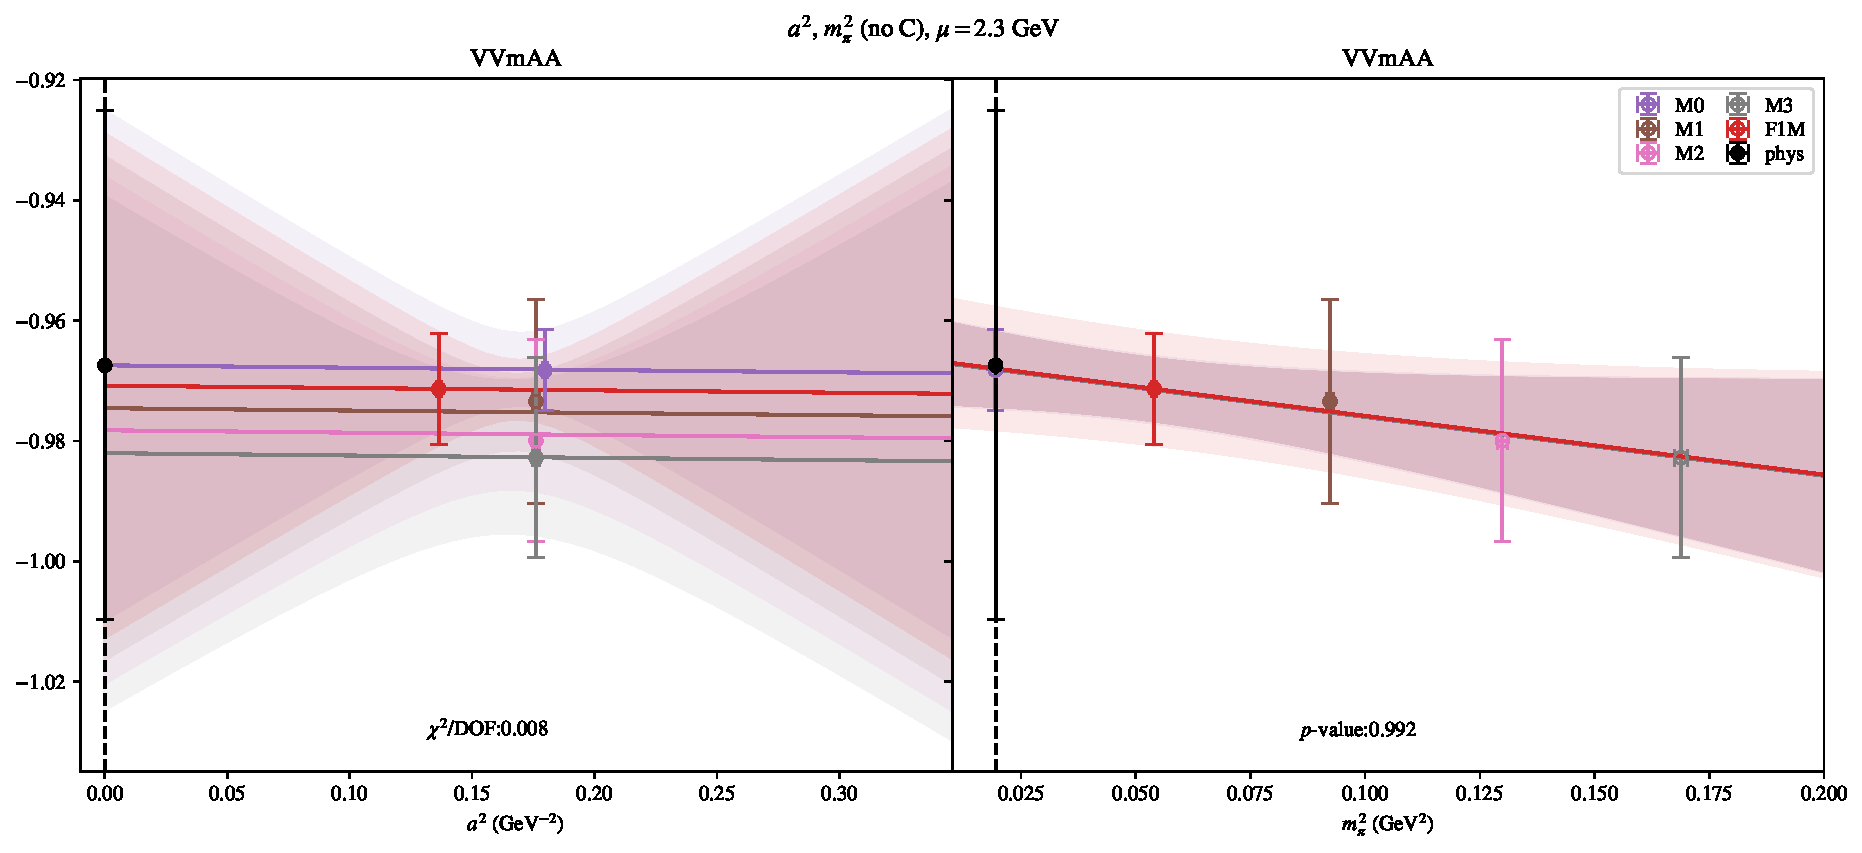
\includepdf[link, pages=-]{VVmAA/NPR/bag_a2m2noC_23.pdf}
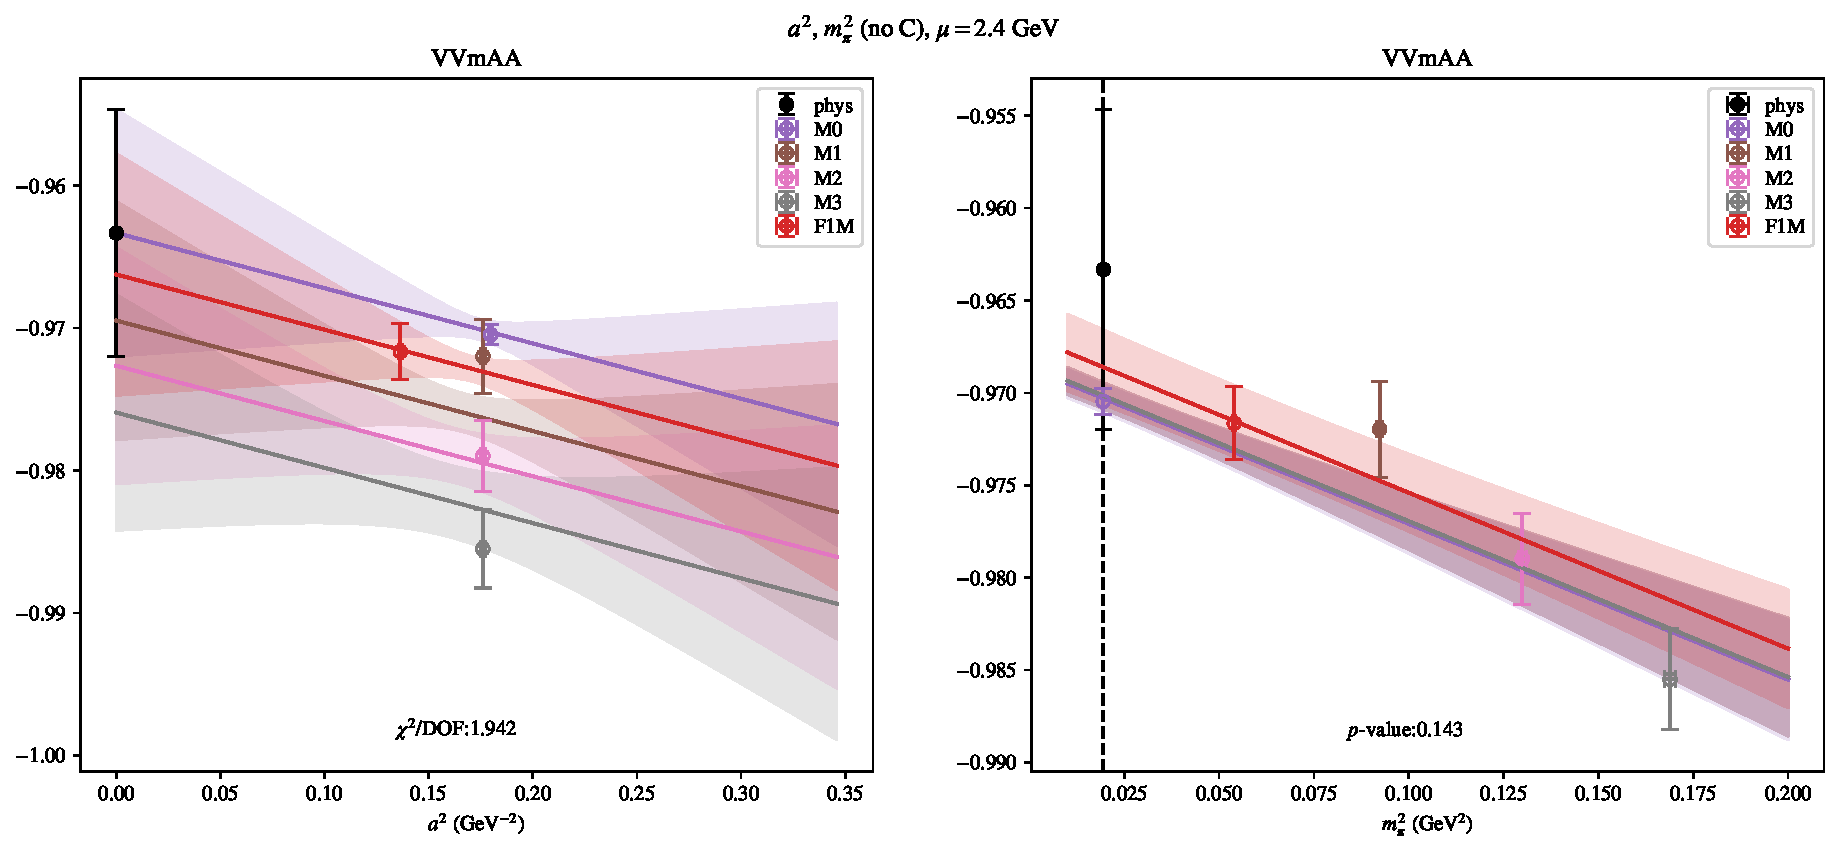
\includepdf[link, pages=-]{VVmAA/NPR/bag_a2m2noC_24.pdf}
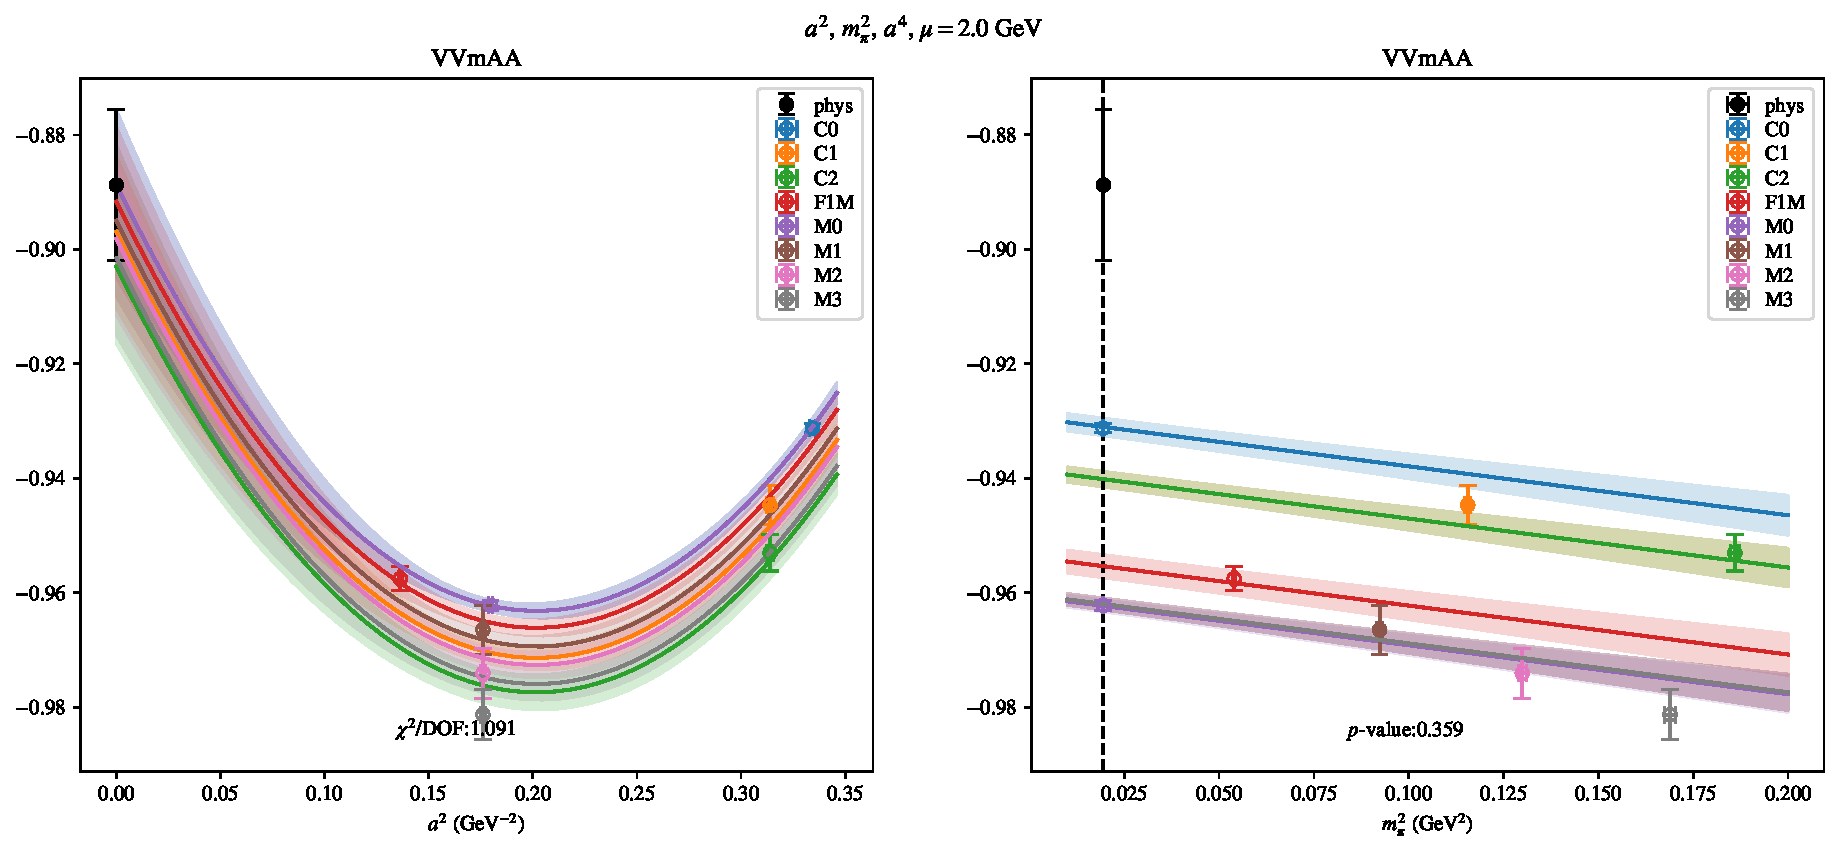
\includepdf[link, pages=-]{VVmAA/NPR/bag_a2a4m2_20.pdf}
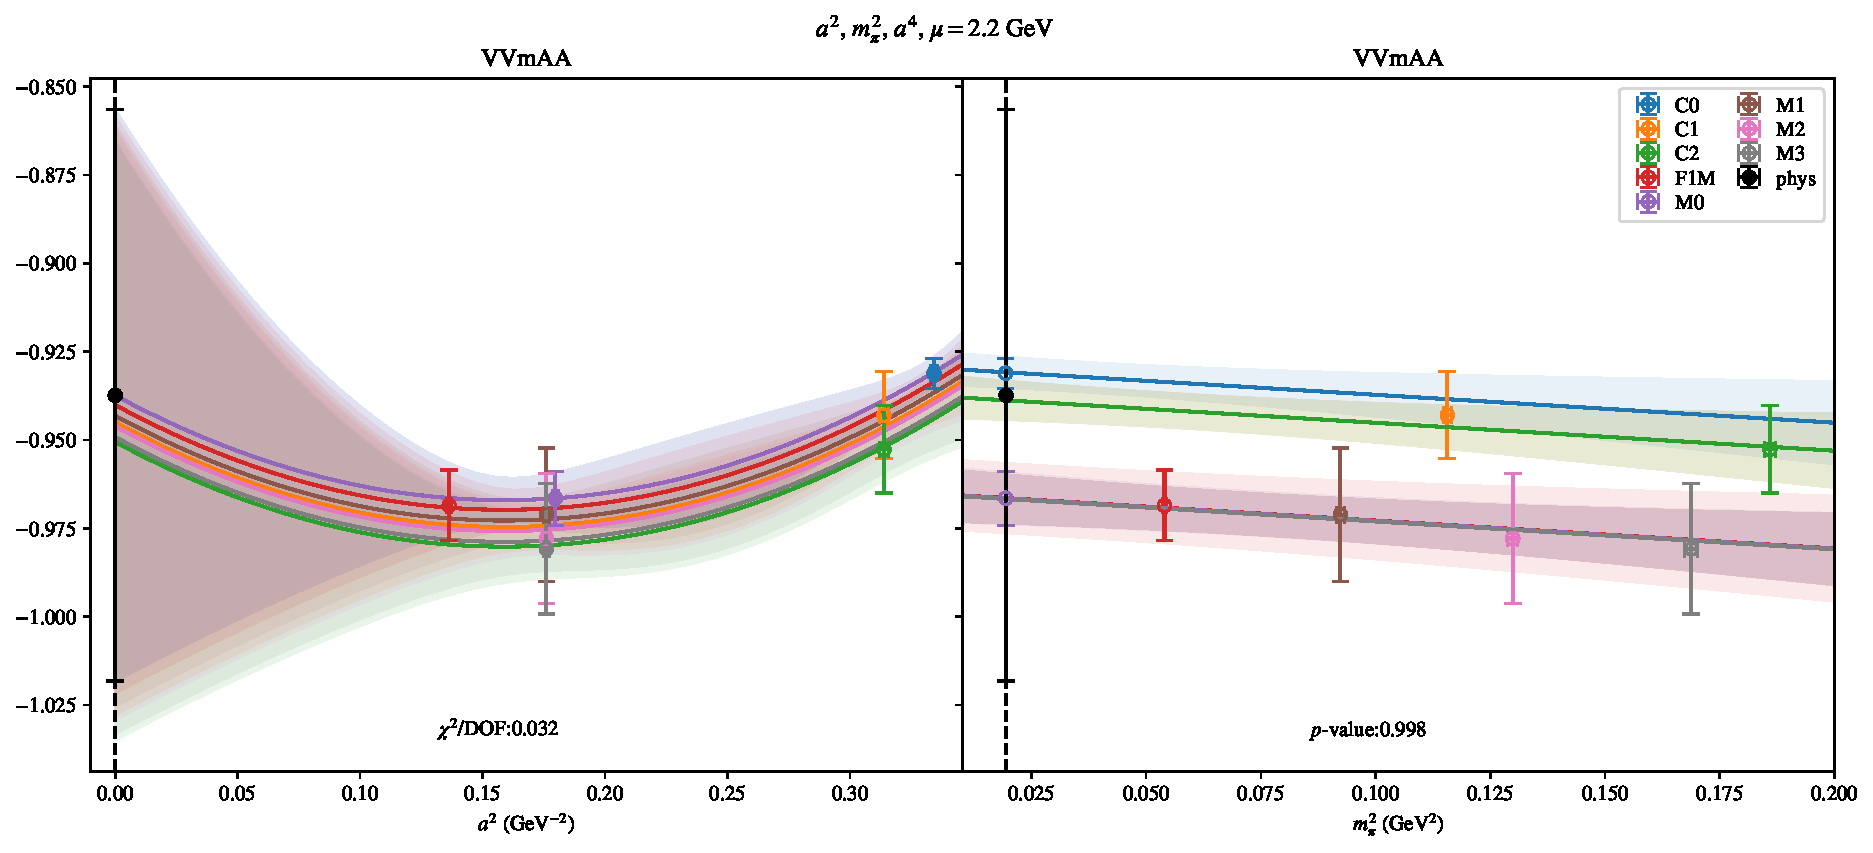
\includepdf[link, pages=-]{VVmAA/NPR/bag_a2a4m2_22.pdf}
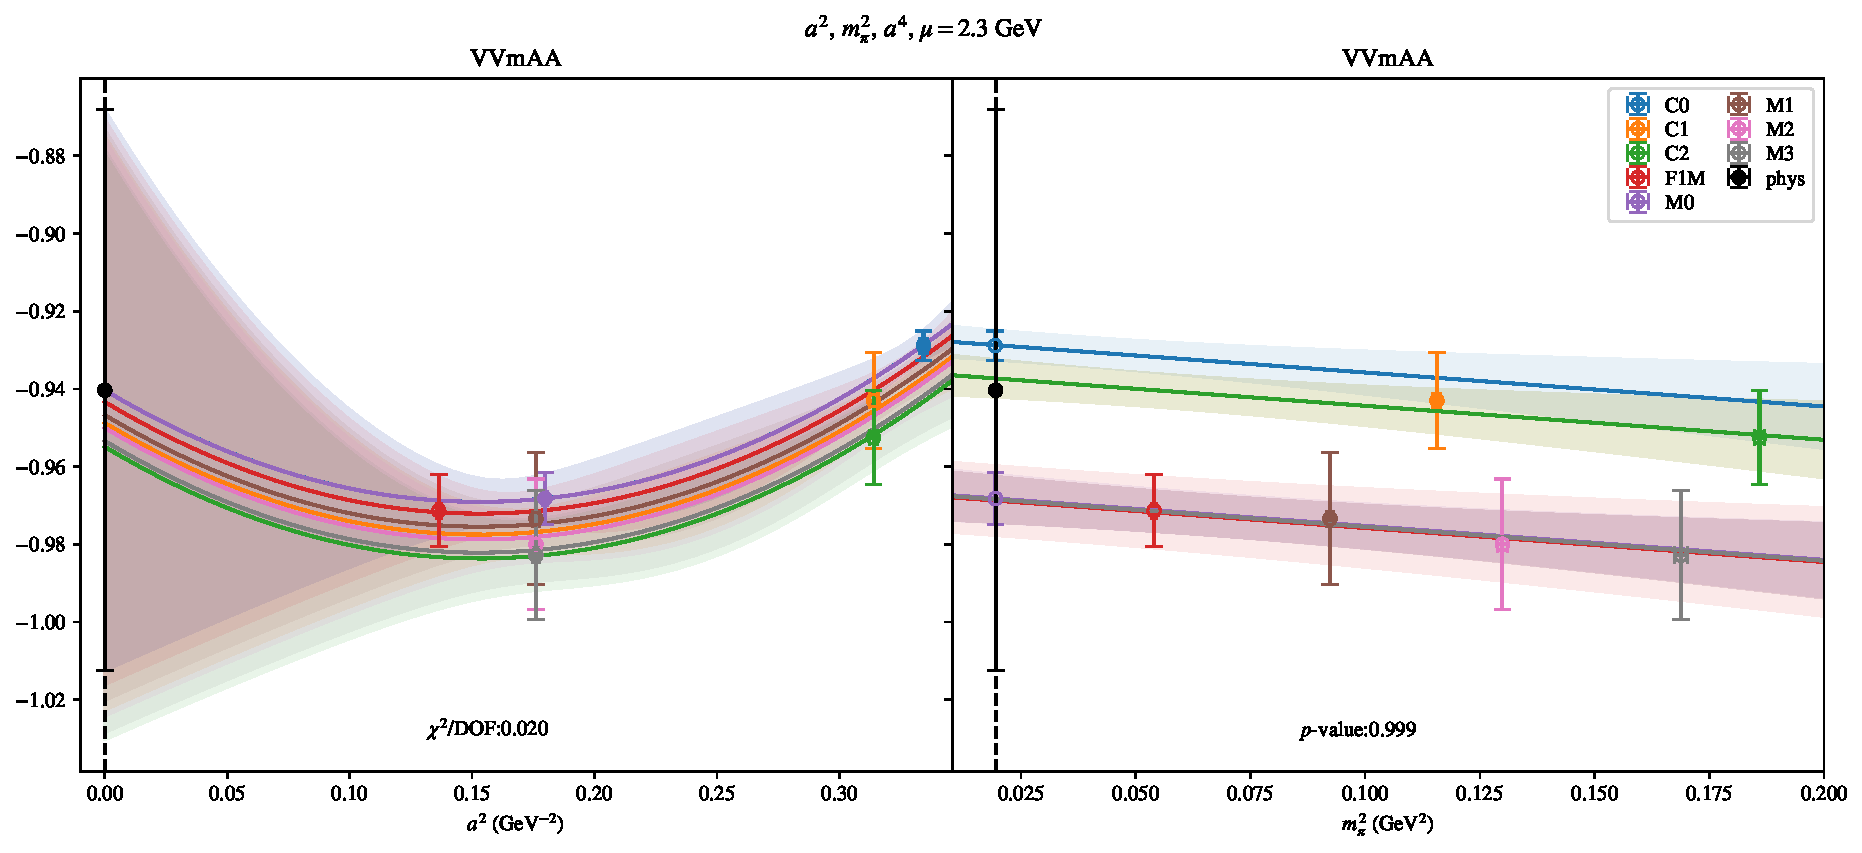
\includepdf[link, pages=-]{VVmAA/NPR/bag_a2a4m2_23.pdf}
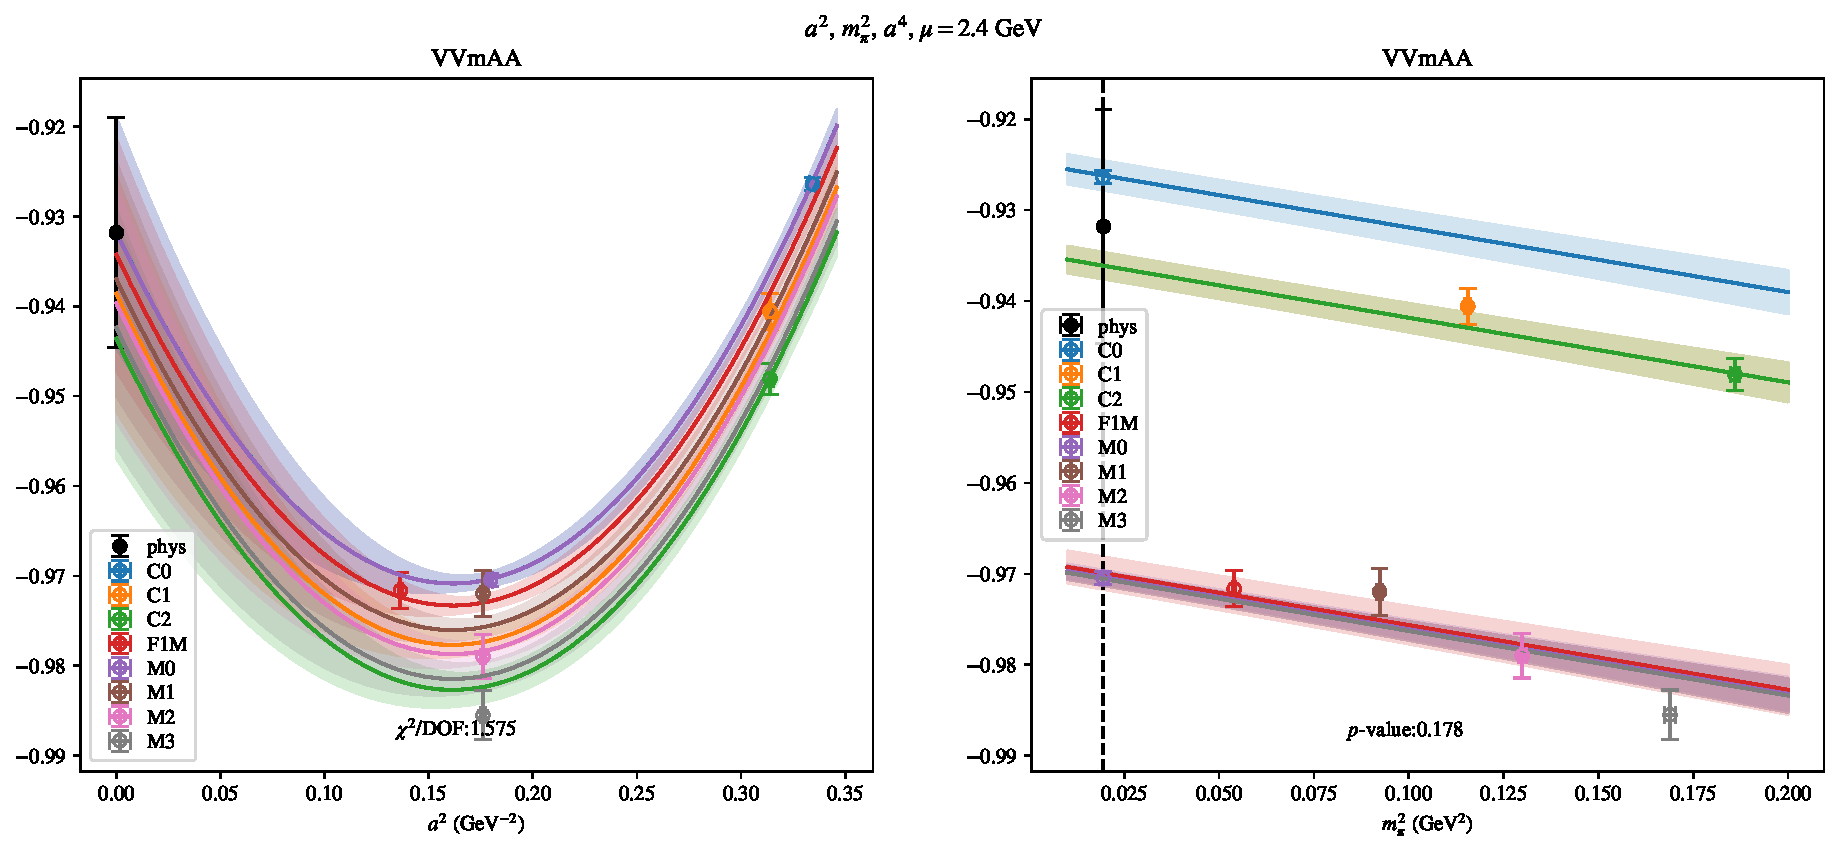
\includepdf[link, pages=-]{VVmAA/NPR/bag_a2a4m2_24.pdf}
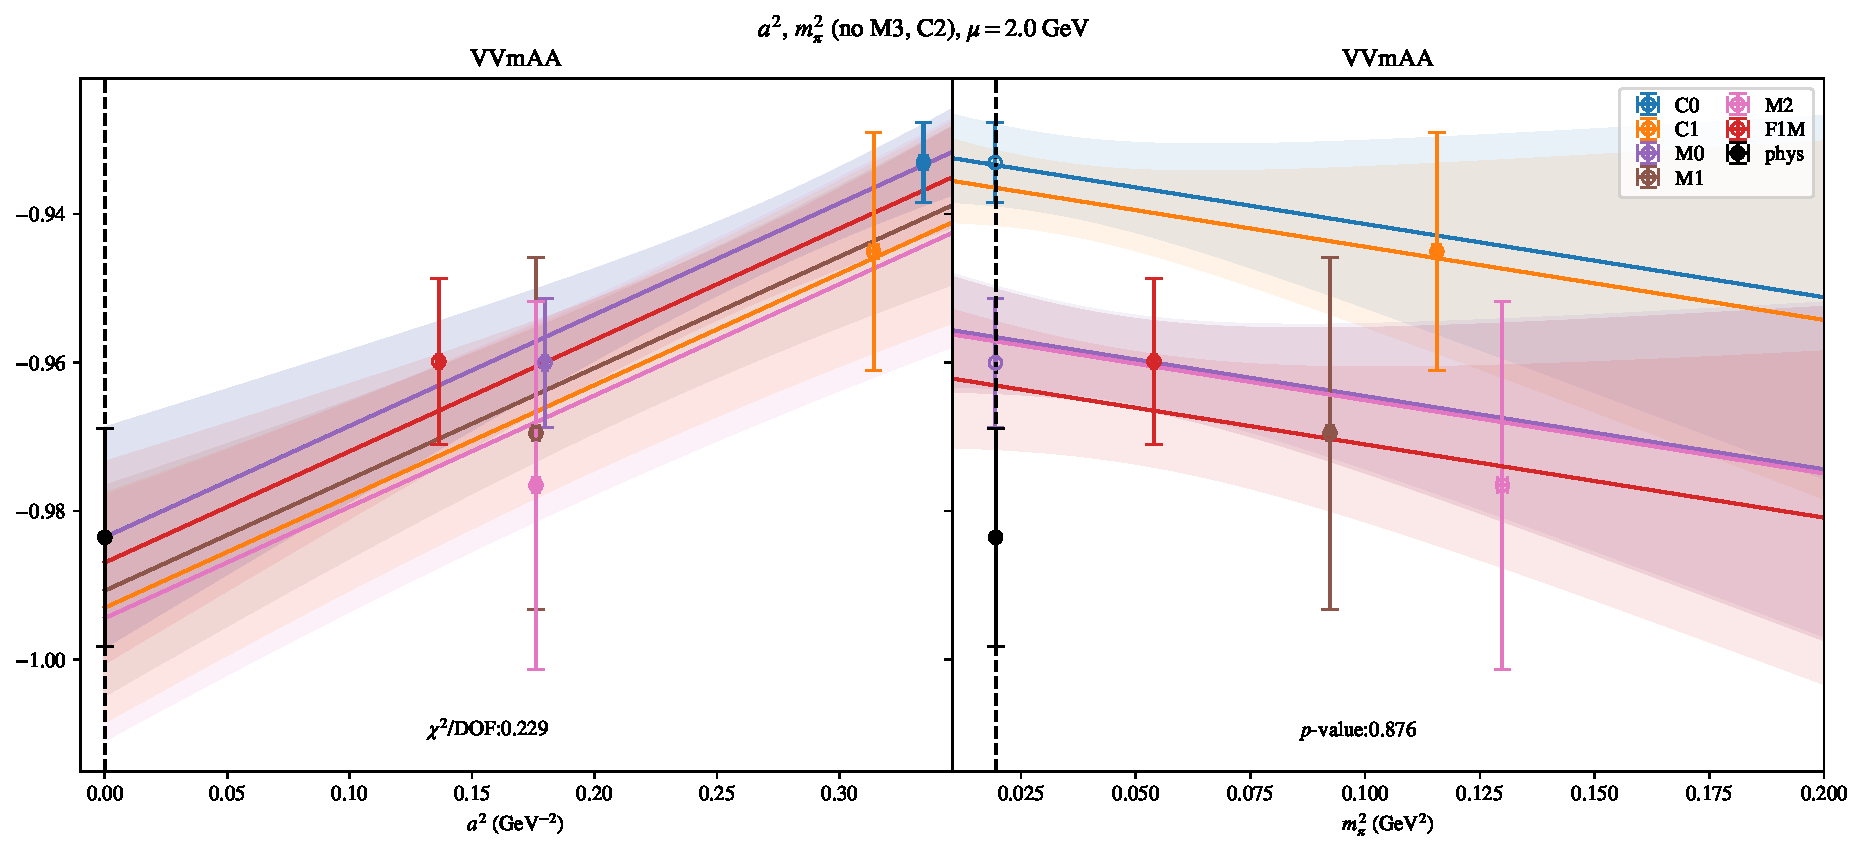
\includepdf[link, pages=-]{VVmAA/NPR/bag_a2m2mcut_20.pdf}
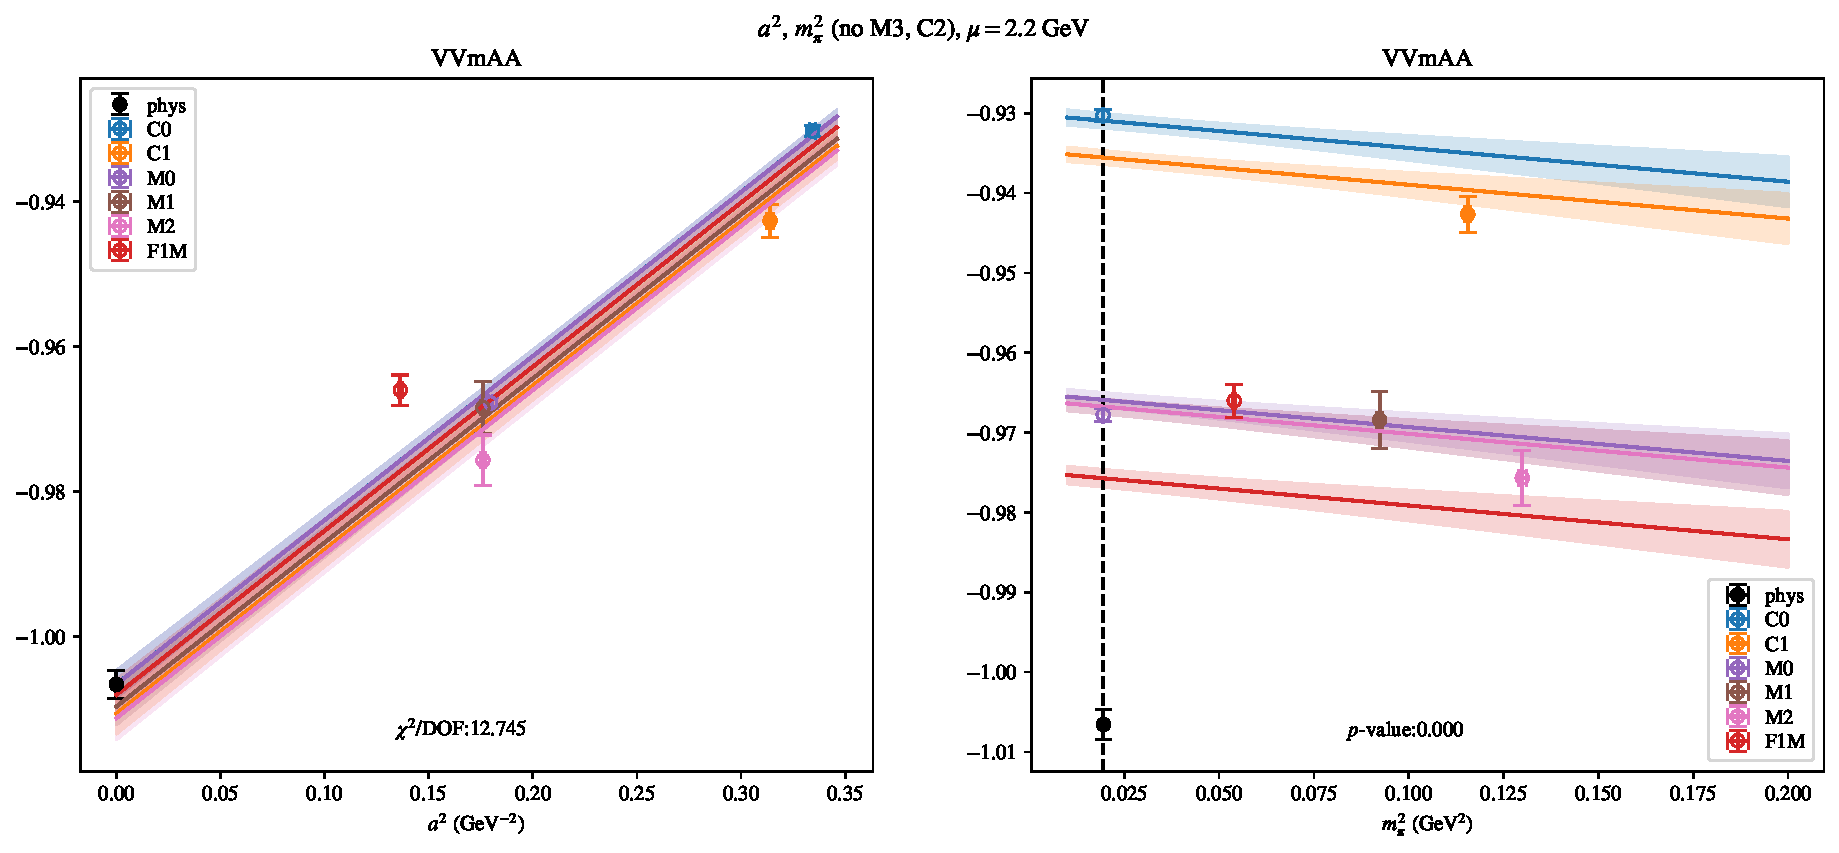
\includepdf[link, pages=-]{VVmAA/NPR/bag_a2m2mcut_22.pdf}
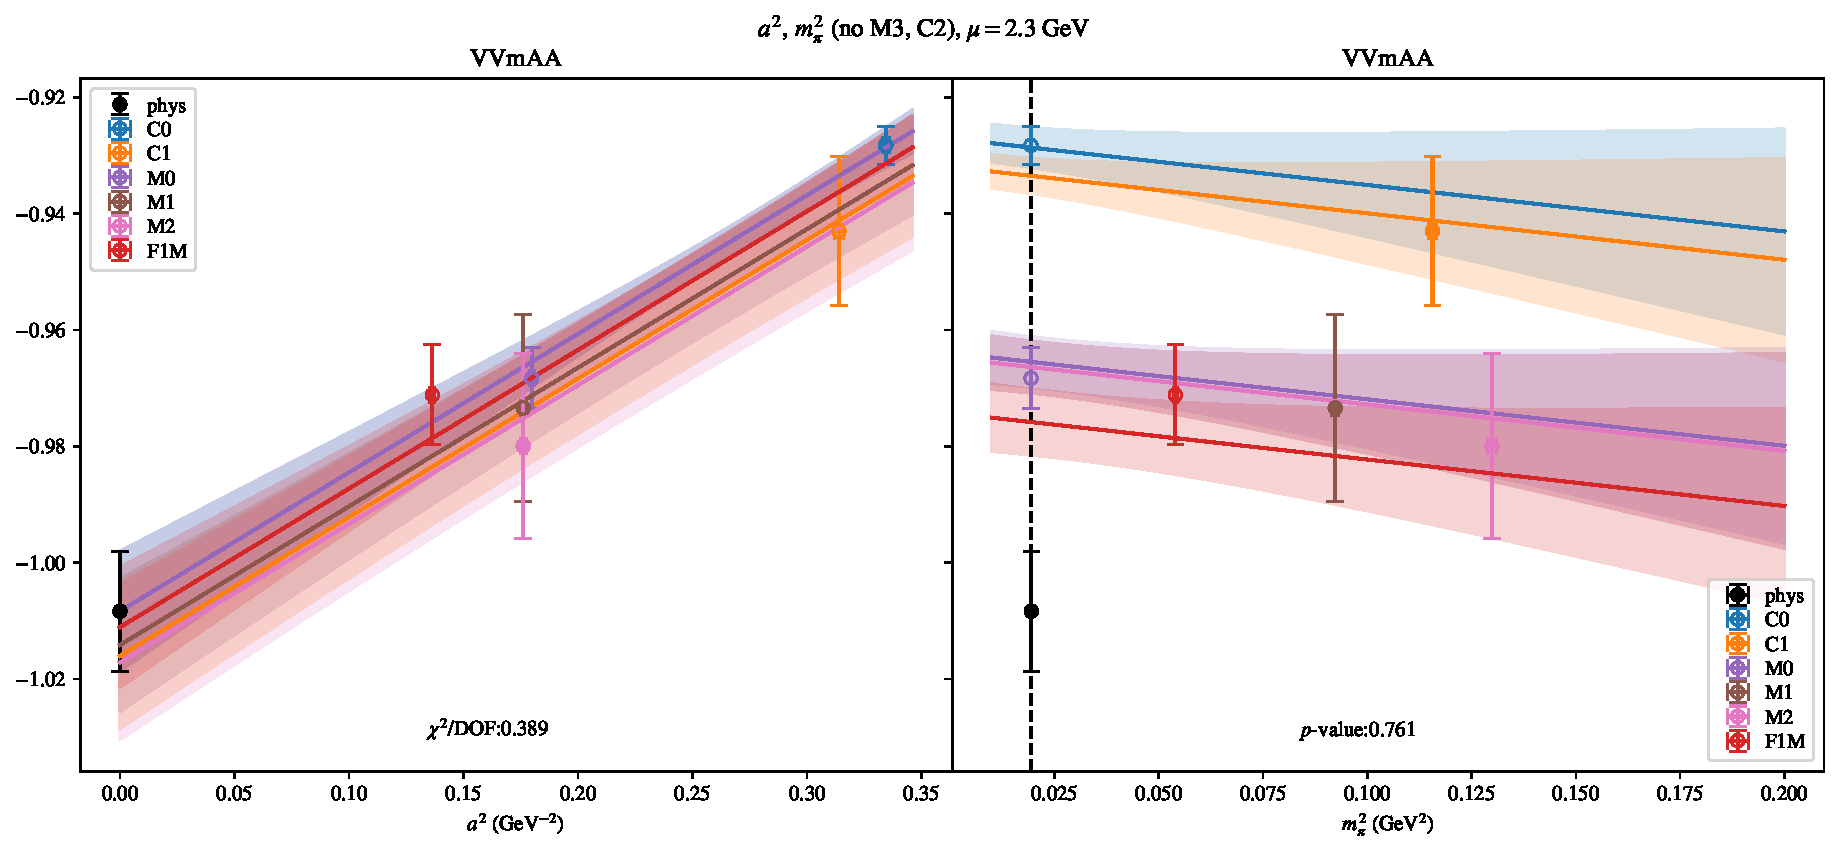
\includepdf[link, pages=-]{VVmAA/NPR/bag_a2m2mcut_23.pdf}
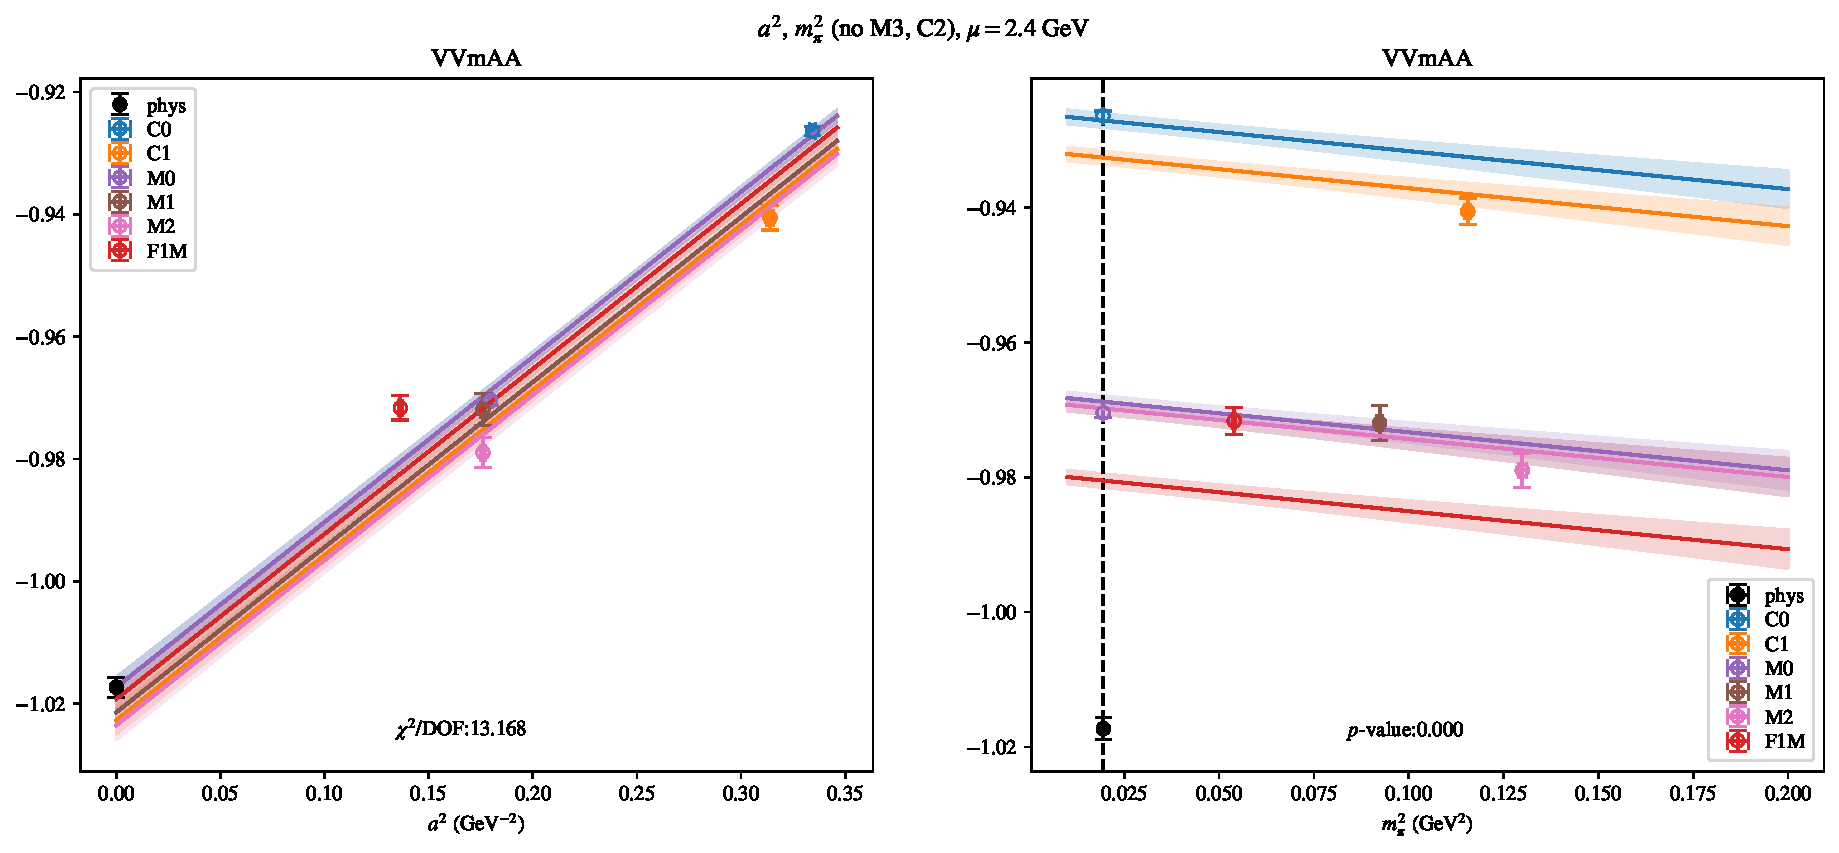
\includepdf[link, pages=-]{VVmAA/NPR/bag_a2m2mcut_24.pdf}
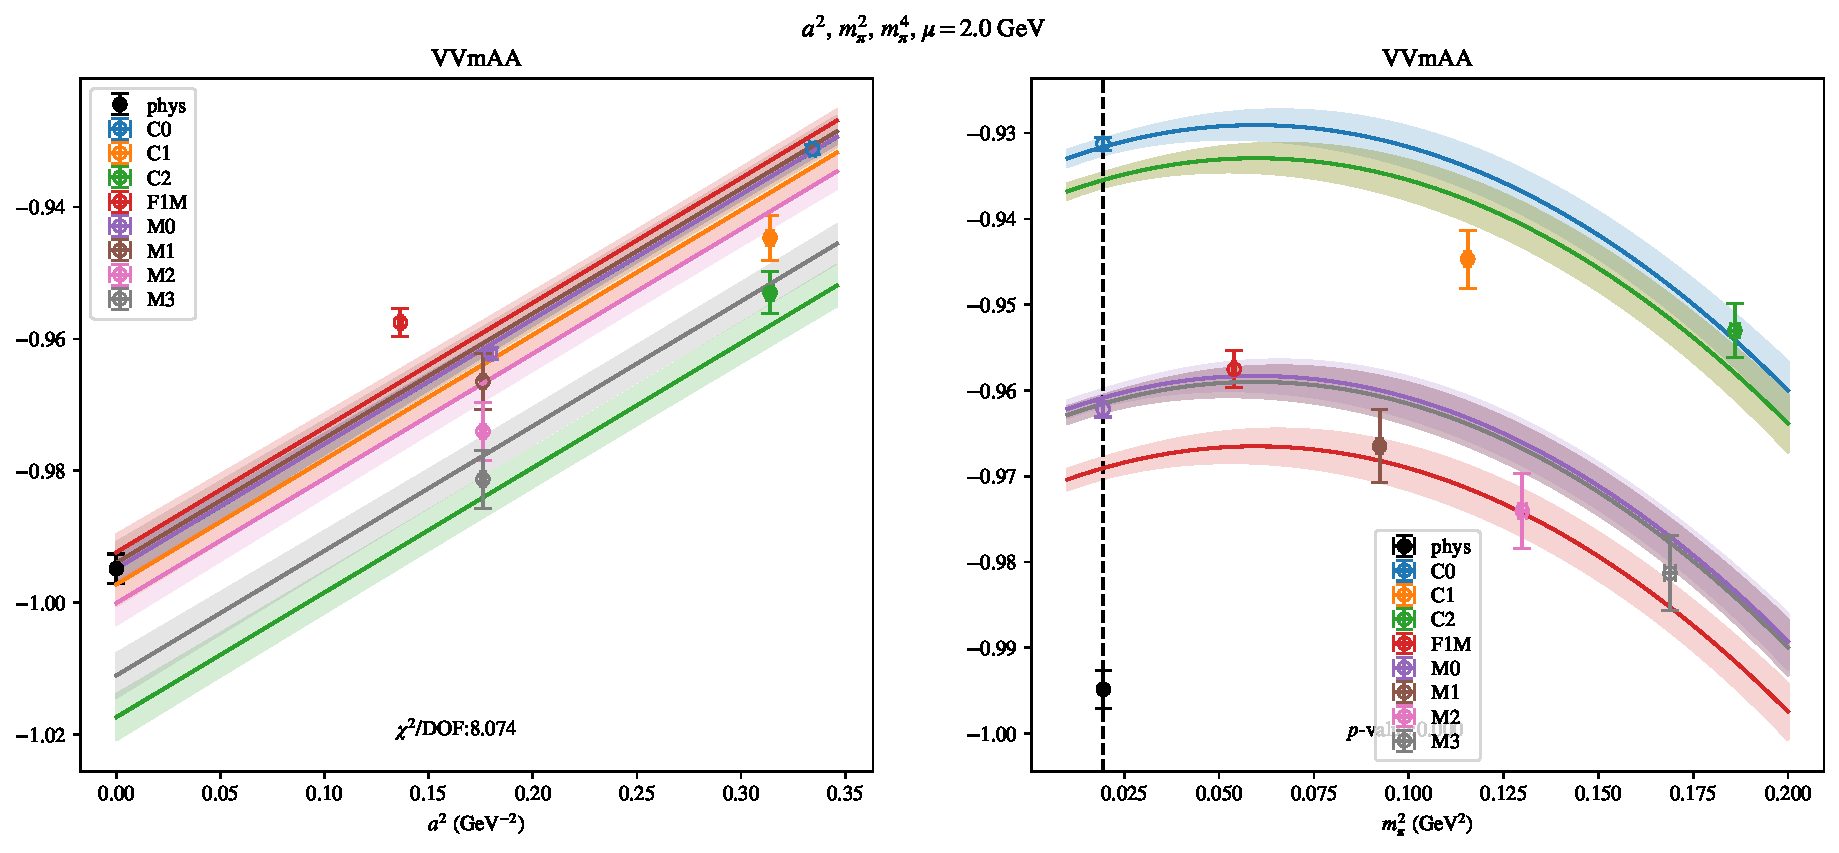
\includepdf[link, pages=-]{VVmAA/NPR/bag_a2m2m4_20.pdf}
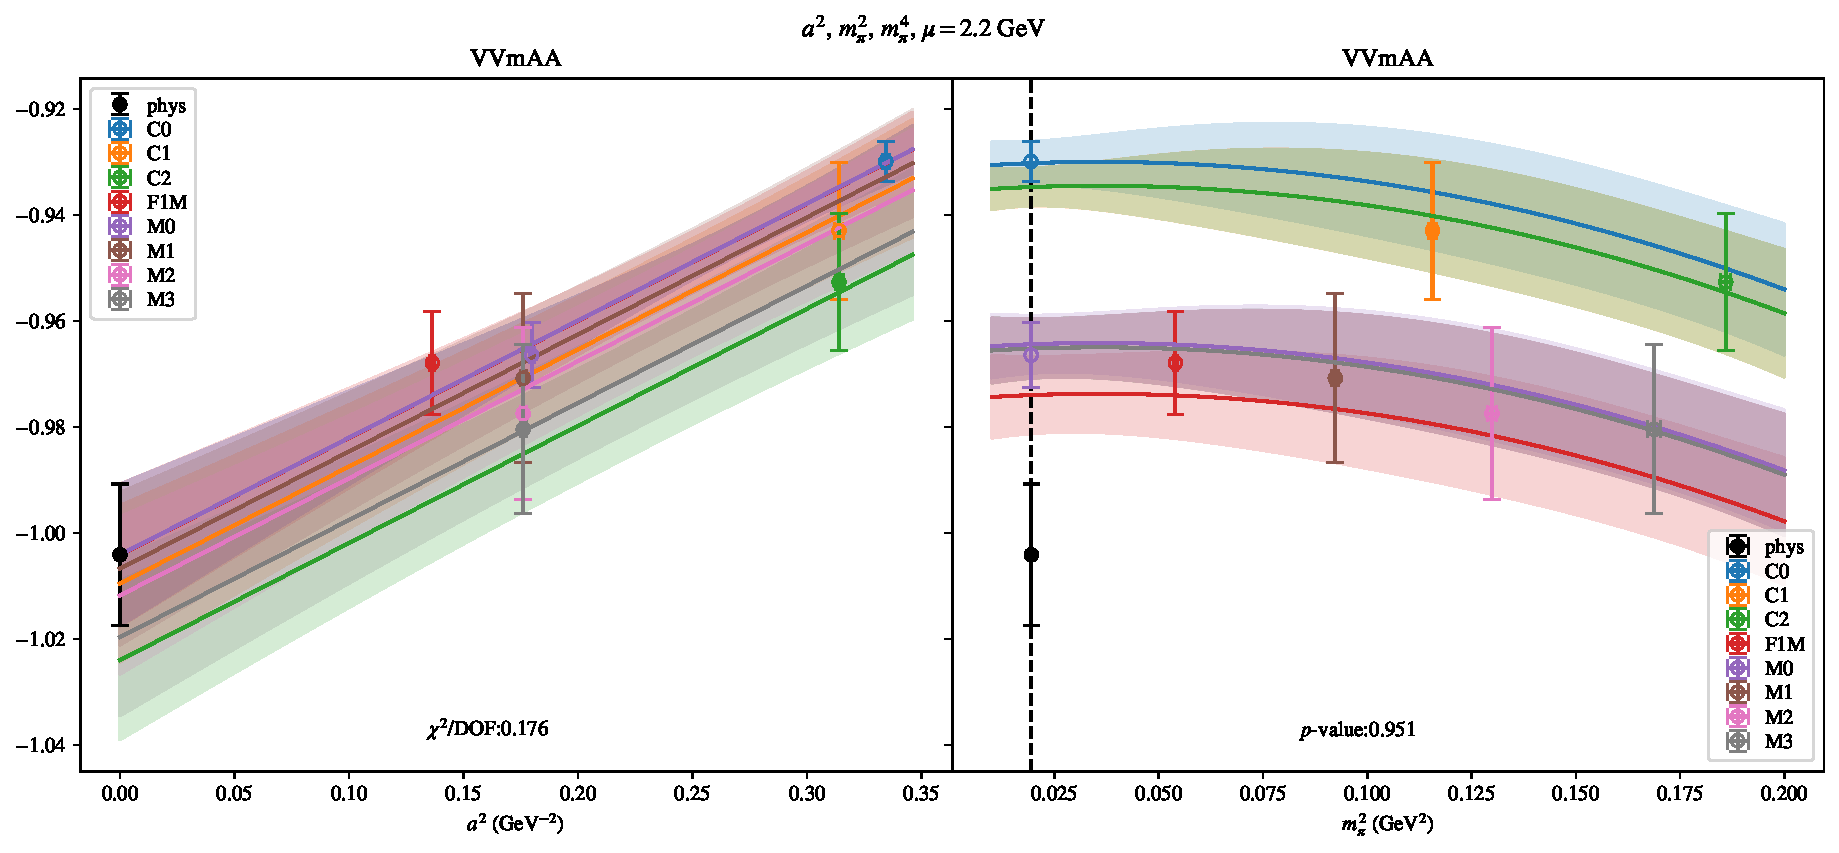
\includepdf[link, pages=-]{VVmAA/NPR/bag_a2m2m4_22.pdf}
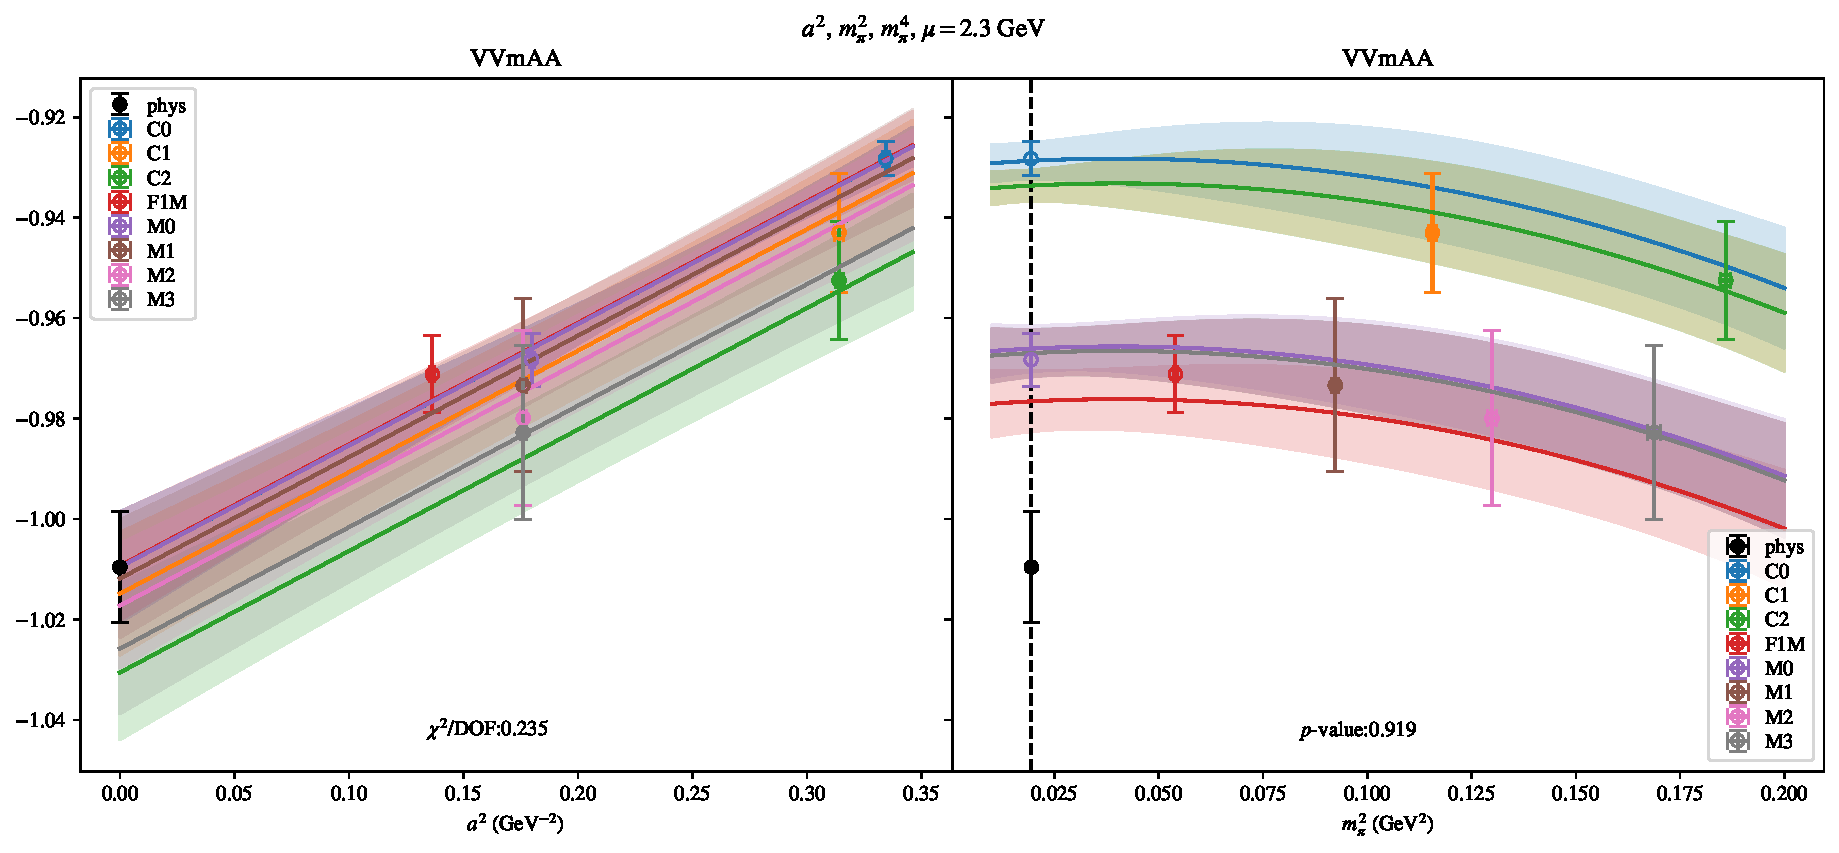
\includepdf[link, pages=-]{VVmAA/NPR/bag_a2m2m4_23.pdf}
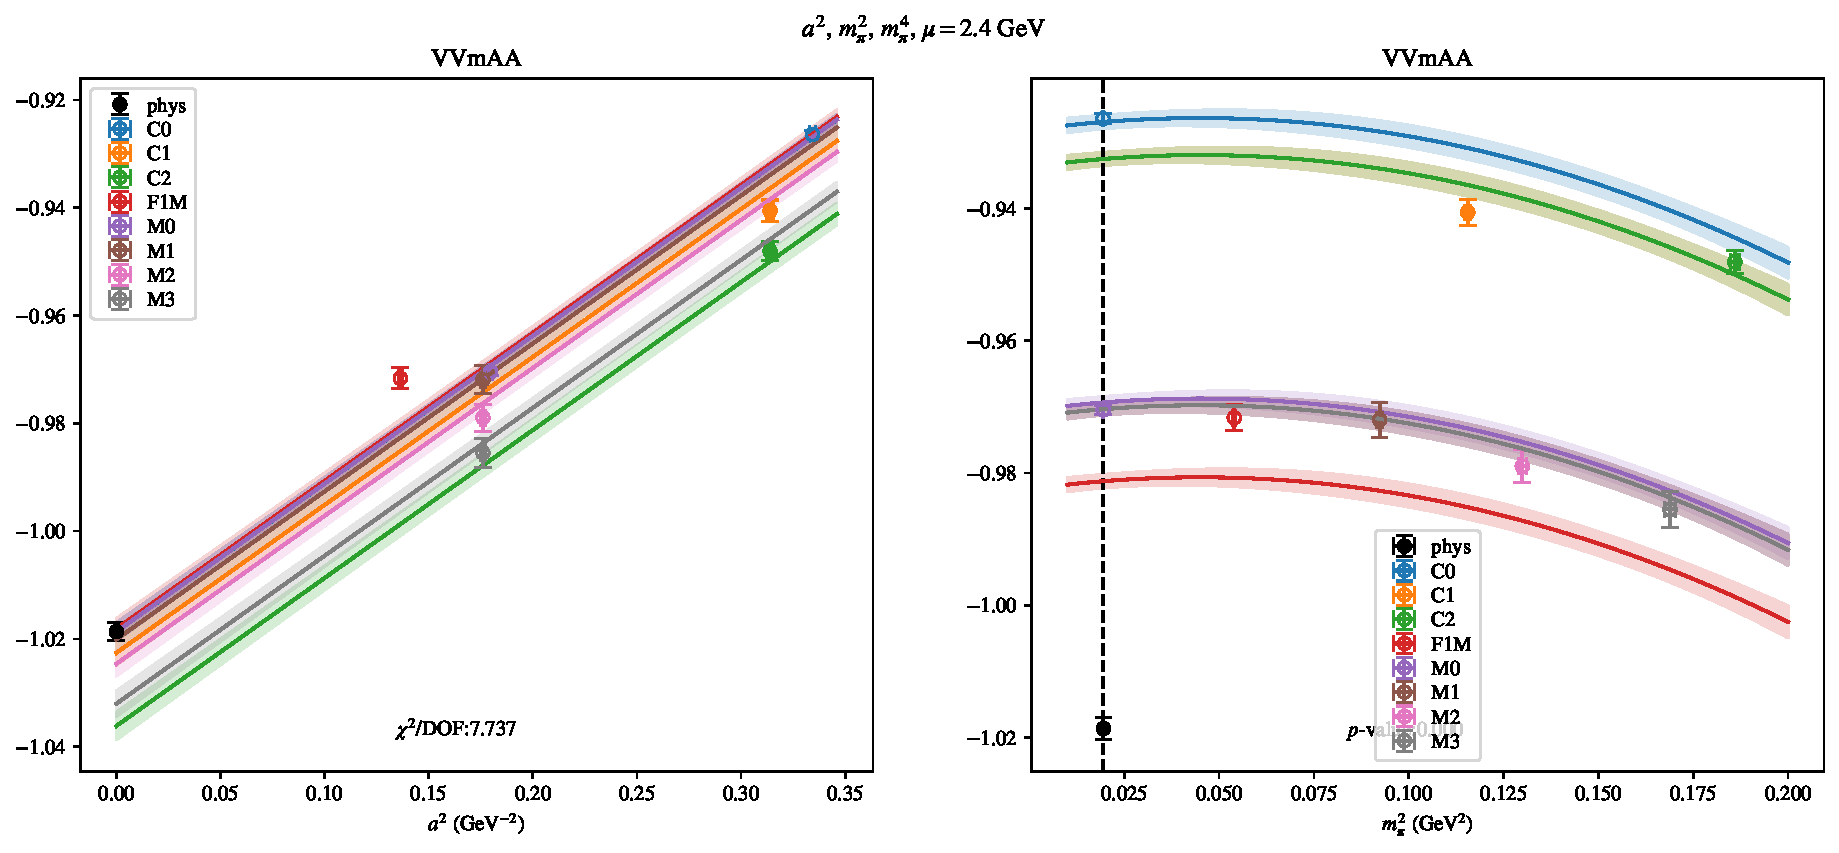
\includepdf[link, pages=-]{VVmAA/NPR/bag_a2m2m4_24.pdf}
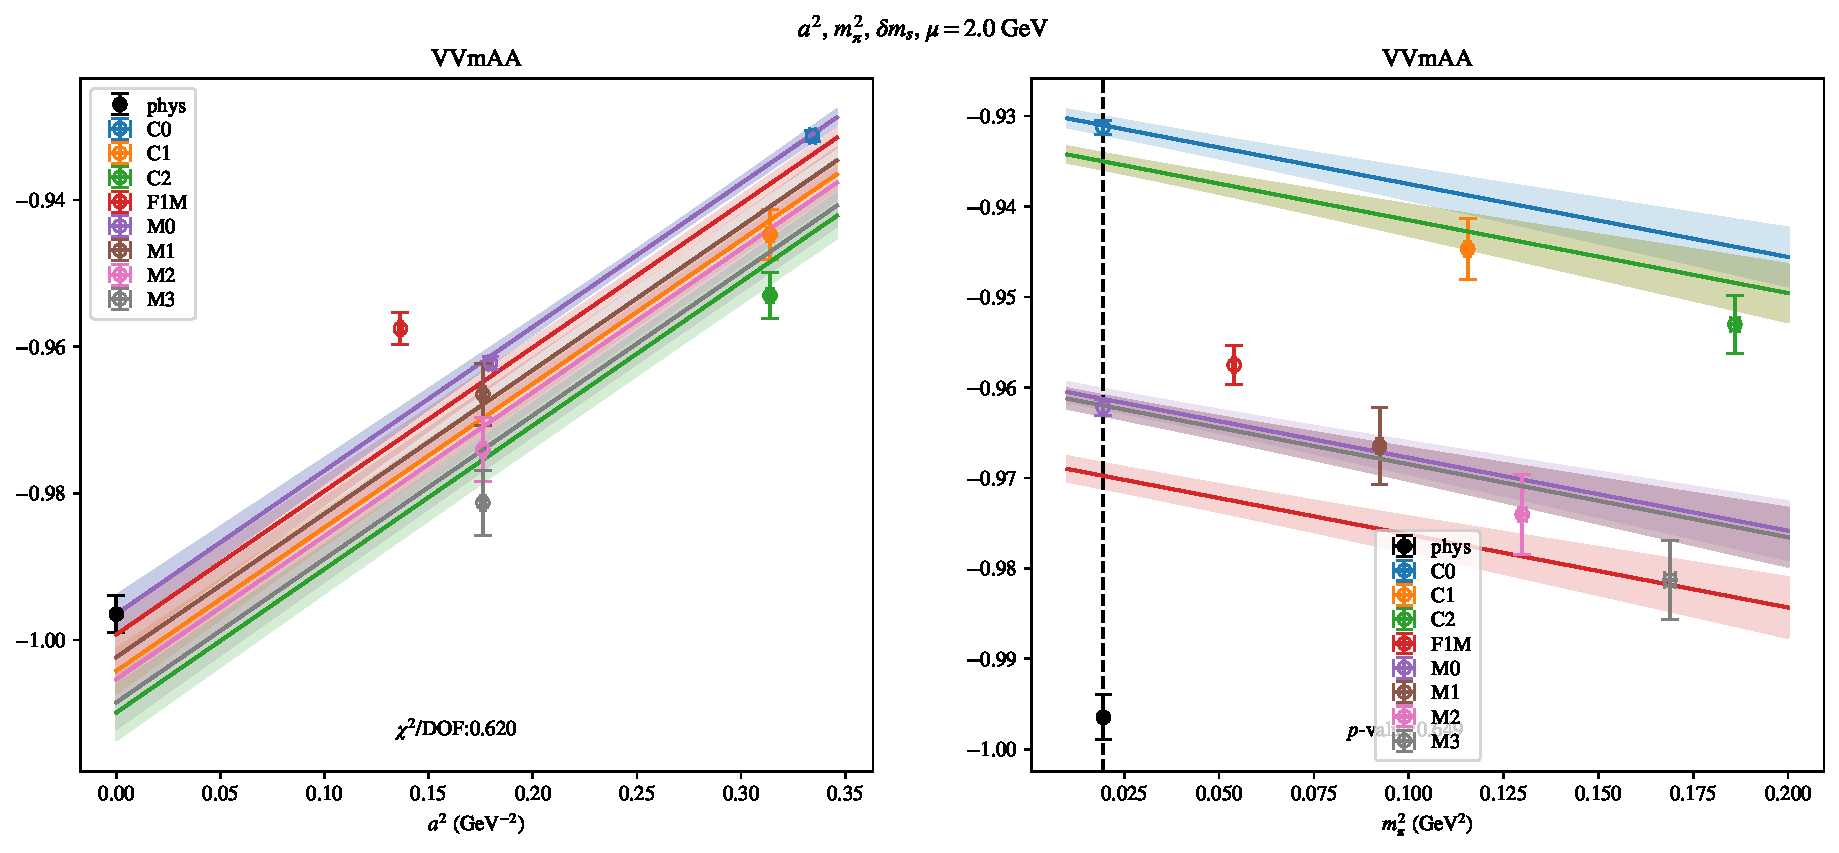
\includepdf[link, pages=-]{VVmAA/NPR/bag_a2m2delm_20.pdf}
\includepdf[link, pages=-]{VVmAA/NPR/bag_a2m2delm_22.pdf}
\includepdf[link, pages=-]{VVmAA/NPR/bag_a2m2delm_23.pdf}
\includepdf[link, pages=-]{VVmAA/NPR/bag_a2m2delm_24.pdf}
\clearpage
\section{$\mathcal{B}_3$}
\begin{table}[h!]
\begin{center}
\begin{tabular}{|c|c|c|c|c|c|c|}
\hline
$\mu$ (GeV) & $a^2$, $m_\pi^2$& $a^2$, $m_\pi^2$ (no C)& $a^2$, $m_\pi^2$, $a^4$& $a^2$, $m_\pi^2$ (no M3, C2)& $a^2$, $m_\pi^2$, $m_\pi^4$& $a^2$, $m_\pi^2$, $\delta m_s$\\
\hline
2.0& \hyperlink{SSmPP/NPR/bag_a2m2_20.pdf.1}{\textbf{1.8009(39)}: 14.74 (0.0)} & \hyperlink{SSmPP/NPR/bag_a2m2noC_20.pdf.1}{\textbf{1.681(14)}: 0.218 (0.804)} & \hyperlink{SSmPP/NPR/bag_a2a4m2_20.pdf.1}{\textbf{1.608(19)}: 1.029 (0.391)} & \hyperlink{SSmPP/NPR/bag_a2m2mcut_20.pdf.1}{\textbf{1.8026(35)}: 21.834 (0.0)} & \hyperlink{SSmPP/NPR/bag_a2m2m4_20.pdf.1}{\textbf{1.8089(38)}: 11.537 (0.0)} & \hyperlink{SSmPP/NPR/bag_a2m2delm_20.pdf.1}{\textbf{1.8143(45)}: 0.389 (0.817)}\\
2.2& \hyperlink{SSmPP/NPR/bag_a2m2_22.pdf.1}{\textbf{1.8069(34)}: 14.185 (0.0)} & \hyperlink{SSmPP/NPR/bag_a2m2noC_22.pdf.1}{\textbf{1.700(13)}: 0.722 (0.486)} & \hyperlink{SSmPP/NPR/bag_a2a4m2_22.pdf.1}{\textbf{1.635(19)}: 1.347 (0.25)} & \hyperlink{SSmPP/NPR/bag_a2m2mcut_22.pdf.1}{\textbf{1.8080(31)}: 21.36 (0.0)} & \hyperlink{SSmPP/NPR/bag_a2m2m4_22.pdf.1}{\textbf{1.8125(33)}: 12.495 (0.0)} & \hyperlink{SSmPP/NPR/bag_a2m2delm_22.pdf.1}{\textbf{1.8177(38)}: 0.983 (0.415)}\\
2.3& \hyperlink{SSmPP/NPR/bag_a2m2_23.pdf.1}{\textbf{1.8085(32)}: 13.916 (0.0)} & \hyperlink{SSmPP/NPR/bag_a2m2noC_23.pdf.1}{\textbf{1.706(12)}: 0.918 (0.399)} & \hyperlink{SSmPP/NPR/bag_a2a4m2_23.pdf.1}{\textbf{1.641(19)}: 1.196 (0.31)} & \hyperlink{SSmPP/NPR/bag_a2m2mcut_23.pdf.1}{\textbf{1.8096(30)}: 21.218 (0.0)} & \hyperlink{SSmPP/NPR/bag_a2m2m4_23.pdf.1}{\textbf{1.8138(32)}: 12.615 (0.0)} & \hyperlink{SSmPP/NPR/bag_a2m2delm_23.pdf.1}{\textbf{1.8186(36)}: 1.167 (0.323)}\\
2.4& \hyperlink{SSmPP/NPR/bag_a2m2_24.pdf.1}{\textbf{1.8103(30)}: 13.489 (0.0)} & \hyperlink{SSmPP/NPR/bag_a2m2noC_24.pdf.1}{\textbf{1.711(12)}: 1.092 (0.335)} & \hyperlink{SSmPP/NPR/bag_a2a4m2_24.pdf.1}{\textbf{1.649(19)}: 1.368 (0.242)} & \hyperlink{SSmPP/NPR/bag_a2m2mcut_24.pdf.1}{\textbf{1.8112(29)}: 20.775 (0.0)} & \hyperlink{SSmPP/NPR/bag_a2m2m4_24.pdf.1}{\textbf{1.8152(30)}: 12.791 (0.0)} & \hyperlink{SSmPP/NPR/bag_a2m2delm_24.pdf.1}{\textbf{1.8194(33)}: 1.343 (0.251)}\\
\hline
\end{tabular}
\caption{Physical point value from chiral and continuum extrapolation at renormalisation scale $\mu$. Entries are \textbf{value(error)}: $\chi^2/\text{DOF}$ ($p$-value).}
\end{center}
\end{table}
\begin{table}[h!]
\begin{center}
\begin{tabular}{|c c|c|c|c|c|c|c|}
\hline
$\mu$ (GeV) &  & $a^2$, $m_\pi^2$& $a^2$, $m_\pi^2$ (no C)& $a^2$, $m_\pi^2$, $a^4$& $a^2$, $m_\pi^2$ (no M3, C2)& $a^2$, $m_\pi^2$, $m_\pi^4$& $a^2$, $m_\pi^2$, $\delta m_s$\\
\hline
\multirow{3}{0.5in}{2.0} & $\alpha$ & 0.129(14)& 0.830(83)& 1.87(17)& 0.124(13)& 0.103(14)& 0.082(16)\\
 & $\beta$ & -0.00100(47)& -0.00007(92)& -0.00117(47)& -0.00253(70)& -0.0112(14)& -0.00132(47)\\
 & $\gamma$ &  &  & -3.50(36)&  & 0.00097(12)& 0.0311(34)\\
\hline
\multirow{3}{0.5in}{2.2} & $\alpha$ & 0.135(12)& 0.759(76)& 1.68(17)& 0.132(11)& 0.117(12)& 0.096(13)\\
 & $\beta$ & -0.00111(31)& -0.00078(70)& -0.00160(31)& -0.00216(52)& -0.0078(12)& -0.00162(31)\\
 & $\gamma$ &  &  & -3.11(35)&  & 0.00061(10)& 0.0276(32)\\
\hline
\multirow{3}{0.5in}{2.3} & $\alpha$ & 0.140(12)& 0.739(75)& 1.65(17)& 0.137(11)& 0.123(11)& 0.104(13)\\
 & $\beta$ & -0.00086(29)& -0.00073(58)& -0.00136(29)& -0.00178(49)& -0.0069(12)& -0.00140(29)\\
 & $\gamma$ &  &  & -3.04(36)&  & 0.00056(10)& 0.0265(33)\\
\hline
\multirow{3}{0.5in}{2.4} & $\alpha$ & 0.142(11)& 0.723(74)& 1.60(17)& 0.140(11)& 0.126(11)& 0.109(12)\\
 & $\beta$ & -0.00075(26)& -0.00065(50)& -0.00126(26)& -0.00150(45)& -0.0059(11)& -0.00130(26)\\
 & $\gamma$ &  &  & -2.93(35)&  & 0.00047(10)& 0.0255(32)\\
\hline
\end{tabular}
\caption{Fit values of coefficients in $Q = Q_{phys} + \mathbf{\alpha} a^2 + \mathbf{\beta}\left(\frac{m_\pi^2}{f_\pi^2}-\frac{m_{\pi,PDG}^2}{f_\pi^2}\right) + \gamma(\ldots)$}
\end{center}
\end{table}
\includepdf[link, pages=-]{SSmPP/NPR/bag_a2m2_20.pdf}
\includepdf[link, pages=-]{SSmPP/NPR/bag_a2m2_22.pdf}
\includepdf[link, pages=-]{SSmPP/NPR/bag_a2m2_23.pdf}
\includepdf[link, pages=-]{SSmPP/NPR/bag_a2m2_24.pdf}
\includepdf[link, pages=-]{SSmPP/NPR/bag_a2m2noC_20.pdf}
\includepdf[link, pages=-]{SSmPP/NPR/bag_a2m2noC_22.pdf}
\includepdf[link, pages=-]{SSmPP/NPR/bag_a2m2noC_23.pdf}
\includepdf[link, pages=-]{SSmPP/NPR/bag_a2m2noC_24.pdf}
\includepdf[link, pages=-]{SSmPP/NPR/bag_a2a4m2_20.pdf}
\includepdf[link, pages=-]{SSmPP/NPR/bag_a2a4m2_22.pdf}
\includepdf[link, pages=-]{SSmPP/NPR/bag_a2a4m2_23.pdf}
\includepdf[link, pages=-]{SSmPP/NPR/bag_a2a4m2_24.pdf}
\includepdf[link, pages=-]{SSmPP/NPR/bag_a2m2mcut_20.pdf}
\includepdf[link, pages=-]{SSmPP/NPR/bag_a2m2mcut_22.pdf}
\includepdf[link, pages=-]{SSmPP/NPR/bag_a2m2mcut_23.pdf}
\includepdf[link, pages=-]{SSmPP/NPR/bag_a2m2mcut_24.pdf}
\includepdf[link, pages=-]{SSmPP/NPR/bag_a2m2m4_20.pdf}
\includepdf[link, pages=-]{SSmPP/NPR/bag_a2m2m4_22.pdf}
\includepdf[link, pages=-]{SSmPP/NPR/bag_a2m2m4_23.pdf}
\includepdf[link, pages=-]{SSmPP/NPR/bag_a2m2m4_24.pdf}
\includepdf[link, pages=-]{SSmPP/NPR/bag_a2m2delm_20.pdf}
\includepdf[link, pages=-]{SSmPP/NPR/bag_a2m2delm_22.pdf}
\includepdf[link, pages=-]{SSmPP/NPR/bag_a2m2delm_23.pdf}
\includepdf[link, pages=-]{SSmPP/NPR/bag_a2m2delm_24.pdf}
\clearpage
\section{$\mathcal{B}_4$}
\begin{table}[h!]
\begin{center}
\begin{tabular}{|c|c|c|c|c|c|c|}
\hline
$\mu$ (GeV) & $a^2$, $m_\pi^2$& $a^2$, $m_\pi^2$ (no C)& $a^2$, $m_\pi^2$, $a^4$& $a^2$, $m_\pi^2$ (no M3, C2)& $a^2$, $m_\pi^2$, $m_\pi^4$& $a^2$, $m_\pi^2$, $\delta m_s$\\
\hline
2.0& \hyperlink{SSpPP/NPR/bag_a2m2_20.pdf.1}{\textbf{-0.9283(27)}: 0.635 (0.673)} & \hyperlink{SSpPP/NPR/bag_a2m2noC_20.pdf.1}{\textbf{-0.931(10)}: 0.694 (0.5)} & \hyperlink{SSpPP/NPR/bag_a2a4m2_20.pdf.1}{\textbf{-0.928(16)}: 0.793 (0.529)} & \hyperlink{SSpPP/NPR/bag_a2m2mcut_20.pdf.1}{\textbf{-0.9277(24)}: 0.576 (0.631)} & \hyperlink{SSpPP/NPR/bag_a2m2m4_20.pdf.1}{\textbf{-0.9271(26)}: 0.409 (0.802)} & \hyperlink{SSpPP/NPR/bag_a2m2delm_20.pdf.1}{\textbf{-0.9282(30)}: 0.793 (0.529)}\\
2.2& \hyperlink{SSpPP/NPR/bag_a2m2_22.pdf.1}{\textbf{-0.9078(21)}: 1.674 (0.137)} & \hyperlink{SSpPP/NPR/bag_a2m2noC_22.pdf.1}{\textbf{-0.9178(94)}: 0.897 (0.408)} & \hyperlink{SSpPP/NPR/bag_a2a4m2_22.pdf.1}{\textbf{-0.911(15)}: 2.083 (0.08)} & \hyperlink{SSpPP/NPR/bag_a2m2mcut_22.pdf.1}{\textbf{-0.9076(20)}: 1.678 (0.169)} & \hyperlink{SSpPP/NPR/bag_a2m2m4_22.pdf.1}{\textbf{-0.9066(21)}: 1.344 (0.251)} & \hyperlink{SSpPP/NPR/bag_a2m2delm_22.pdf.1}{\textbf{-0.9074(23)}: 2.006 (0.091)}\\
2.3& \hyperlink{SSpPP/NPR/bag_a2m2_23.pdf.1}{\textbf{-0.8985(19)}: 2.517 (0.028)} & \hyperlink{SSpPP/NPR/bag_a2m2noC_23.pdf.1}{\textbf{-0.9112(91)}: 1.268 (0.281)} & \hyperlink{SSpPP/NPR/bag_a2a4m2_23.pdf.1}{\textbf{-0.902(14)}: 3.13 (0.014)} & \hyperlink{SSpPP/NPR/bag_a2m2mcut_23.pdf.1}{\textbf{-0.8985(18)}: 2.722 (0.043)} & \hyperlink{SSpPP/NPR/bag_a2m2m4_23.pdf.1}{\textbf{-0.8973(20)}: 2.306 (0.056)} & \hyperlink{SSpPP/NPR/bag_a2m2delm_23.pdf.1}{\textbf{-0.8980(21)}: 2.973 (0.018)}\\
2.4& \hyperlink{SSpPP/NPR/bag_a2m2_24.pdf.1}{\textbf{-0.8904(18)}: 3.166 (0.007)} & \hyperlink{SSpPP/NPR/bag_a2m2noC_24.pdf.1}{\textbf{-0.9044(89)}: 1.546 (0.213)} & \hyperlink{SSpPP/NPR/bag_a2a4m2_24.pdf.1}{\textbf{-0.894(14)}: 3.944 (0.003)} & \hyperlink{SSpPP/NPR/bag_a2m2mcut_24.pdf.1}{\textbf{-0.8906(18)}: 3.492 (0.015)} & \hyperlink{SSpPP/NPR/bag_a2m2m4_24.pdf.1}{\textbf{-0.8891(19)}: 3.071 (0.015)} & \hyperlink{SSpPP/NPR/bag_a2m2delm_24.pdf.1}{\textbf{-0.8899(20)}: 3.728 (0.005)}\\
\hline
\end{tabular}
\caption{Physical point value from chiral and continuum extrapolation at renormalisation scale $\mu$. Entries are \textbf{value(error)}: $\chi^2/\text{DOF}$ ($p$-value).}
\end{center}
\end{table}
\begin{table}[h!]
\begin{center}
\begin{tabular}{|c c|c|c|c|c|c|c|}
\hline
$\mu$ (GeV) &  & $a^2$, $m_\pi^2$& $a^2$, $m_\pi^2$ (no C)& $a^2$, $m_\pi^2$, $a^4$& $a^2$, $m_\pi^2$ (no M3, C2)& $a^2$, $m_\pi^2$, $m_\pi^4$& $a^2$, $m_\pi^2$, $\delta m_s$\\
\hline
\multirow{3}{0.5in}{2.0} & $\alpha$ & -0.341(10)& -0.328(62)& -0.35(14)& -0.3427(95)& -0.345(10)& -0.341(11)\\
 & $\beta$ & -0.00699(30)& -0.00686(58)& -0.00699(30)& -0.00742(43)& -0.00855(96)& -0.00699(30)\\
 & $\gamma$ &  &  & 0.01(28)&  & 0.000148(76)& 0.00002(263)\\
\hline
\multirow{3}{0.5in}{2.2} & $\alpha$ & -0.3763(82)& -0.321(55)& -0.35(13)& -0.3765(79)& -0.3801(82)& -0.3778(86)\\
 & $\beta$ & -0.00672(19)& -0.00633(38)& -0.00673(19)& -0.00711(30)& -0.00824(77)& -0.00675(19)\\
 & $\gamma$ &  &  & -0.05(27)&  & 0.000139(63)& 0.0014(24)\\
\hline
\multirow{3}{0.5in}{2.3} & $\alpha$ & -0.3944(77)& -0.325(53)& -0.36(13)& -0.3939(75)& -0.3985(77)& -0.3962(79)\\
 & $\beta$ & -0.00678(17)& -0.00631(32)& -0.00679(18)& -0.00714(28)& -0.00828(74)& -0.00682(18)\\
 & $\gamma$ &  &  & -0.07(26)&  & 0.000138(62)& 0.0019(23)\\
\hline
\multirow{3}{0.5in}{2.4} & $\alpha$ & -0.4095(72)& -0.333(52)& -0.38(13)& -0.4084(72)& -0.4137(73)& -0.4114(74)\\
 & $\beta$ & -0.00675(15)& -0.00626(27)& -0.00676(16)& -0.00709(26)& -0.00821(71)& -0.00681(16)\\
 & $\gamma$ &  &  & -0.06(26)&  & 0.000132(61)& 0.0021(22)\\
\hline
\end{tabular}
\caption{Fit values of coefficients in $Q = Q_{phys} + \mathbf{\alpha} a^2 + \mathbf{\beta}\left(\frac{m_\pi^2}{f_\pi^2}-\frac{m_{\pi,PDG}^2}{f_\pi^2}\right) + \gamma(\ldots)$}
\end{center}
\end{table}
\includepdf[link, pages=-]{SSpPP/NPR/bag_a2m2_20.pdf}
\includepdf[link, pages=-]{SSpPP/NPR/bag_a2m2_22.pdf}
\includepdf[link, pages=-]{SSpPP/NPR/bag_a2m2_23.pdf}
\includepdf[link, pages=-]{SSpPP/NPR/bag_a2m2_24.pdf}
\includepdf[link, pages=-]{SSpPP/NPR/bag_a2m2noC_20.pdf}
\includepdf[link, pages=-]{SSpPP/NPR/bag_a2m2noC_22.pdf}
\includepdf[link, pages=-]{SSpPP/NPR/bag_a2m2noC_23.pdf}
\includepdf[link, pages=-]{SSpPP/NPR/bag_a2m2noC_24.pdf}
\includepdf[link, pages=-]{SSpPP/NPR/bag_a2a4m2_20.pdf}
\includepdf[link, pages=-]{SSpPP/NPR/bag_a2a4m2_22.pdf}
\includepdf[link, pages=-]{SSpPP/NPR/bag_a2a4m2_23.pdf}
\includepdf[link, pages=-]{SSpPP/NPR/bag_a2a4m2_24.pdf}
\includepdf[link, pages=-]{SSpPP/NPR/bag_a2m2mcut_20.pdf}
\includepdf[link, pages=-]{SSpPP/NPR/bag_a2m2mcut_22.pdf}
\includepdf[link, pages=-]{SSpPP/NPR/bag_a2m2mcut_23.pdf}
\includepdf[link, pages=-]{SSpPP/NPR/bag_a2m2mcut_24.pdf}
\includepdf[link, pages=-]{SSpPP/NPR/bag_a2m2m4_20.pdf}
\includepdf[link, pages=-]{SSpPP/NPR/bag_a2m2m4_22.pdf}
\includepdf[link, pages=-]{SSpPP/NPR/bag_a2m2m4_23.pdf}
\includepdf[link, pages=-]{SSpPP/NPR/bag_a2m2m4_24.pdf}
\includepdf[link, pages=-]{SSpPP/NPR/bag_a2m2delm_20.pdf}
\includepdf[link, pages=-]{SSpPP/NPR/bag_a2m2delm_22.pdf}
\includepdf[link, pages=-]{SSpPP/NPR/bag_a2m2delm_23.pdf}
\includepdf[link, pages=-]{SSpPP/NPR/bag_a2m2delm_24.pdf}
\clearpage
\section{$\mathcal{B}_5$}
\begin{table}[h!]
\begin{center}
\begin{tabular}{|c|c|c|c|c|c|c|}
\hline
$\mu$ (GeV) & $a^2$, $m_\pi^2$& $a^2$, $m_\pi^2$ (no C)& $a^2$, $m_\pi^2$, $a^4$& $a^2$, $m_\pi^2$ (no M3, C2)& $a^2$, $m_\pi^2$, $m_\pi^4$& $a^2$, $m_\pi^2$, $\delta m_s$\\
\hline
2.0& \hyperlink{TT/NPR/bag_a2m2_20.pdf.1}{\textbf{-0.3627(11)}: 0.322 (0.9)} & \hyperlink{TT/NPR/bag_a2m2noC_20.pdf.1}{\textbf{-0.3639(48)}: 0.138 (0.871)} & \hyperlink{TT/NPR/bag_a2a4m2_20.pdf.1}{\textbf{-0.3608(70)}: 0.387 (0.818)} & \hyperlink{TT/NPR/bag_a2m2mcut_20.pdf.1}{\textbf{-0.3627(10)}: 0.411 (0.745)} & \hyperlink{TT/NPR/bag_a2m2m4_20.pdf.1}{\textbf{-0.3626(10)}: 0.397 (0.811)} & \hyperlink{TT/NPR/bag_a2m2delm_20.pdf.1}{\textbf{-0.3627(12)}: 0.402 (0.807)}\\
2.2& \hyperlink{TT/NPR/bag_a2m2_22.pdf.1}{\textbf{-0.35980(94)}: 0.809 (0.543)} & \hyperlink{TT/NPR/bag_a2m2noC_22.pdf.1}{\textbf{-0.3630(41)}: 0.179 (0.836)} & \hyperlink{TT/NPR/bag_a2a4m2_22.pdf.1}{\textbf{-0.3592(65)}: 1.009 (0.401)} & \hyperlink{TT/NPR/bag_a2m2mcut_22.pdf.1}{\textbf{-0.35998(84)}: 0.978 (0.402)} & \hyperlink{TT/NPR/bag_a2m2m4_22.pdf.1}{\textbf{-0.35978(89)}: 1.01 (0.401)} & \hyperlink{TT/NPR/bag_a2m2delm_22.pdf.1}{\textbf{-0.35970(99)}: 0.97 (0.423)}\\
2.3& \hyperlink{TT/NPR/bag_a2m2_23.pdf.1}{\textbf{-0.35848(86)}: 1.282 (0.268)} & \hyperlink{TT/NPR/bag_a2m2noC_23.pdf.1}{\textbf{-0.3618(40)}: 0.252 (0.777)} & \hyperlink{TT/NPR/bag_a2a4m2_23.pdf.1}{\textbf{-0.3567(63)}: 1.584 (0.175)} & \hyperlink{TT/NPR/bag_a2m2mcut_23.pdf.1}{\textbf{-0.35869(78)}: 1.531 (0.204)} & \hyperlink{TT/NPR/bag_a2m2m4_23.pdf.1}{\textbf{-0.35842(82)}: 1.587 (0.175)} & \hyperlink{TT/NPR/bag_a2m2delm_23.pdf.1}{\textbf{-0.35840(90)}: 1.565 (0.181)}\\
2.4& \hyperlink{TT/NPR/bag_a2m2_24.pdf.1}{\textbf{-0.35736(81)}: 1.359 (0.236)} & \hyperlink{TT/NPR/bag_a2m2noC_24.pdf.1}{\textbf{-0.3607(40)}: 0.321 (0.725)} & \hyperlink{TT/NPR/bag_a2a4m2_24.pdf.1}{\textbf{-0.3557(62)}: 1.681 (0.151)} & \hyperlink{TT/NPR/bag_a2m2mcut_24.pdf.1}{\textbf{-0.35757(73)}: 1.652 (0.175)} & \hyperlink{TT/NPR/bag_a2m2m4_24.pdf.1}{\textbf{-0.35728(77)}: 1.662 (0.156)} & \hyperlink{TT/NPR/bag_a2m2delm_24.pdf.1}{\textbf{-0.35728(85)}: 1.655 (0.157)}\\
\hline
\end{tabular}
\caption{Physical point value from chiral and continuum extrapolation at renormalisation scale $\mu$. Entries are \textbf{value(error)}: $\chi^2/\text{DOF}$ ($p$-value).}
\end{center}
\end{table}
\begin{table}[h!]
\begin{center}
\begin{tabular}{|c c|c|c|c|c|c|c|}
\hline
$\mu$ (GeV) &  & $a^2$, $m_\pi^2$& $a^2$, $m_\pi^2$ (no C)& $a^2$, $m_\pi^2$, $a^4$& $a^2$, $m_\pi^2$ (no M3, C2)& $a^2$, $m_\pi^2$, $m_\pi^4$& $a^2$, $m_\pi^2$, $\delta m_s$\\
\hline
\multirow{3}{0.5in}{2.0} & $\alpha$ & 0.0134(42)& 0.020(28)& -0.003(62)& 0.0137(37)& 0.0133(40)& 0.0135(45)\\
 & $\beta$ & -0.00250(12)& -0.00234(23)& -0.00249(12)& -0.00251(17)& -0.00257(39)& -0.00250(12)\\
 & $\gamma$ &  &  & 0.03(12)&  & 0.000007(30)& -0.00002(118)\\
\hline
\multirow{3}{0.5in}{2.2} & $\alpha$ & 0.0287(34)& 0.046(24)& 0.023(57)& 0.0295(31)& 0.0287(33)& 0.0284(36)\\
 & $\beta$ & -0.002363(84)& -0.00215(17)& -0.002361(87)& -0.00236(13)& -0.00239(32)& -0.002371(87)\\
 & $\gamma$ &  &  & 0.01(11)&  & 0.000003(25)& 0.0004(10)\\
\hline
\multirow{3}{0.5in}{2.3} & $\alpha$ & 0.0360(32)& 0.054(23)& 0.021(55)& 0.0368(29)& 0.0358(31)& 0.0356(33)\\
 & $\beta$ & -0.002416(77)& -0.00220(14)& -0.002411(80)& -0.00243(12)& -0.00251(30)& -0.002424(80)\\
 & $\gamma$ &  &  & 0.03(11)&  & 0.000008(24)& 0.0004(10)\\
\hline
\multirow{3}{0.5in}{2.4} & $\alpha$ & 0.0438(30)& 0.062(22)& 0.029(54)& 0.0446(27)& 0.0435(29)& 0.0435(31)\\
 & $\beta$ & -0.002410(71)& -0.00221(13)& -0.002405(76)& -0.00244(11)& -0.00254(29)& -0.002419(76)\\
 & $\gamma$ &  &  & 0.03(10)&  & 0.000012(23)& 0.00041(99)\\
\hline
\end{tabular}
\caption{Fit values of coefficients in $Q = Q_{phys} + \mathbf{\alpha} a^2 + \mathbf{\beta}\left(\frac{m_\pi^2}{f_\pi^2}-\frac{m_{\pi,PDG}^2}{f_\pi^2}\right) + \gamma(\ldots)$}
\end{center}
\end{table}
\includepdf[link, pages=-]{TT/NPR/bag_a2m2_20.pdf}
\includepdf[link, pages=-]{TT/NPR/bag_a2m2_22.pdf}
\includepdf[link, pages=-]{TT/NPR/bag_a2m2_23.pdf}
\includepdf[link, pages=-]{TT/NPR/bag_a2m2_24.pdf}
\includepdf[link, pages=-]{TT/NPR/bag_a2m2noC_20.pdf}
\includepdf[link, pages=-]{TT/NPR/bag_a2m2noC_22.pdf}
\includepdf[link, pages=-]{TT/NPR/bag_a2m2noC_23.pdf}
\includepdf[link, pages=-]{TT/NPR/bag_a2m2noC_24.pdf}
\includepdf[link, pages=-]{TT/NPR/bag_a2a4m2_20.pdf}
\includepdf[link, pages=-]{TT/NPR/bag_a2a4m2_22.pdf}
\includepdf[link, pages=-]{TT/NPR/bag_a2a4m2_23.pdf}
\includepdf[link, pages=-]{TT/NPR/bag_a2a4m2_24.pdf}
\includepdf[link, pages=-]{TT/NPR/bag_a2m2mcut_20.pdf}
\includepdf[link, pages=-]{TT/NPR/bag_a2m2mcut_22.pdf}
\includepdf[link, pages=-]{TT/NPR/bag_a2m2mcut_23.pdf}
\includepdf[link, pages=-]{TT/NPR/bag_a2m2mcut_24.pdf}
\includepdf[link, pages=-]{TT/NPR/bag_a2m2m4_20.pdf}
\includepdf[link, pages=-]{TT/NPR/bag_a2m2m4_22.pdf}
\includepdf[link, pages=-]{TT/NPR/bag_a2m2m4_23.pdf}
\includepdf[link, pages=-]{TT/NPR/bag_a2m2m4_24.pdf}
\includepdf[link, pages=-]{TT/NPR/bag_a2m2delm_20.pdf}
\includepdf[link, pages=-]{TT/NPR/bag_a2m2delm_22.pdf}
\includepdf[link, pages=-]{TT/NPR/bag_a2m2delm_23.pdf}
\includepdf[link, pages=-]{TT/NPR/bag_a2m2delm_24.pdf}
\clearpage
\end{document}